%%____________________________________________________________________________||
\section{MHT post-fit templates}
\label{sec:mht_postfit_templates}

In Figures ~\ref{fig:postFitShapes_eq0b_eq2a}-~\ref{fig:postFitShapes_ge3b_ge5j} the post-fit \MHT templates are shown for all the analysis bins where the \MHT templates are used.


\clearpage
\newpage
\begin{figure}[h!]
\caption{Post-fit \MHT templates for the bin $\nj^{\mathrm{asym}}=2$, $\nb=0$ \label{fig:postFitShapes_eq0b_eq2a}}.
\begin{center}

    \subfigure[$\nj^{\mathrm{asym}}=2$, $\nb=0$, $200 < \scalht < 250 \; \mathrm{GeV}$]{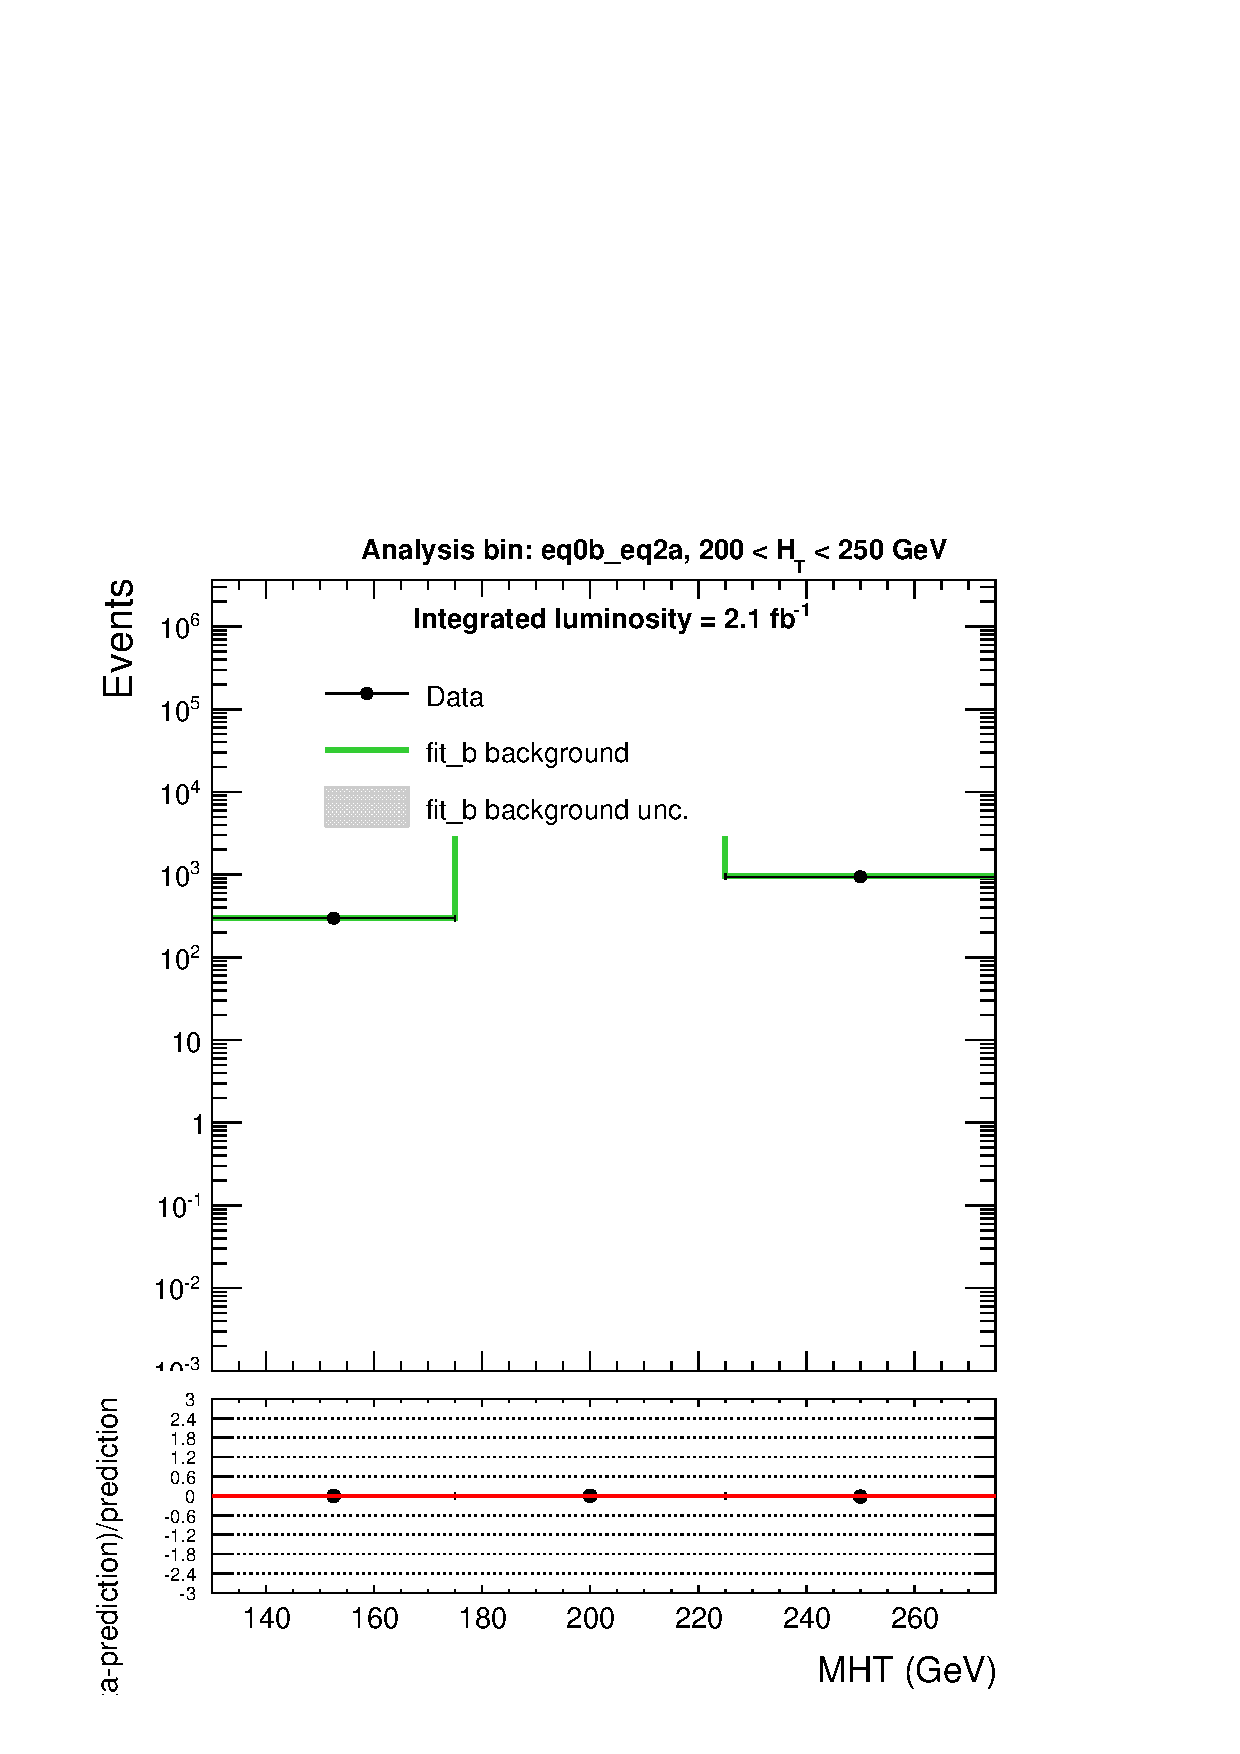
\includegraphics[width=0.25\textwidth]{figures/postFitResults/postFitShapes/postFitShape_eq0b_eq2a_200_250.pdf} }\hspace{1cm}
    \subfigure[$\nj^{\mathrm{asym}}=2$, $\nb=0$, $250 < \scalht < 300 \; \mathrm{GeV}$]{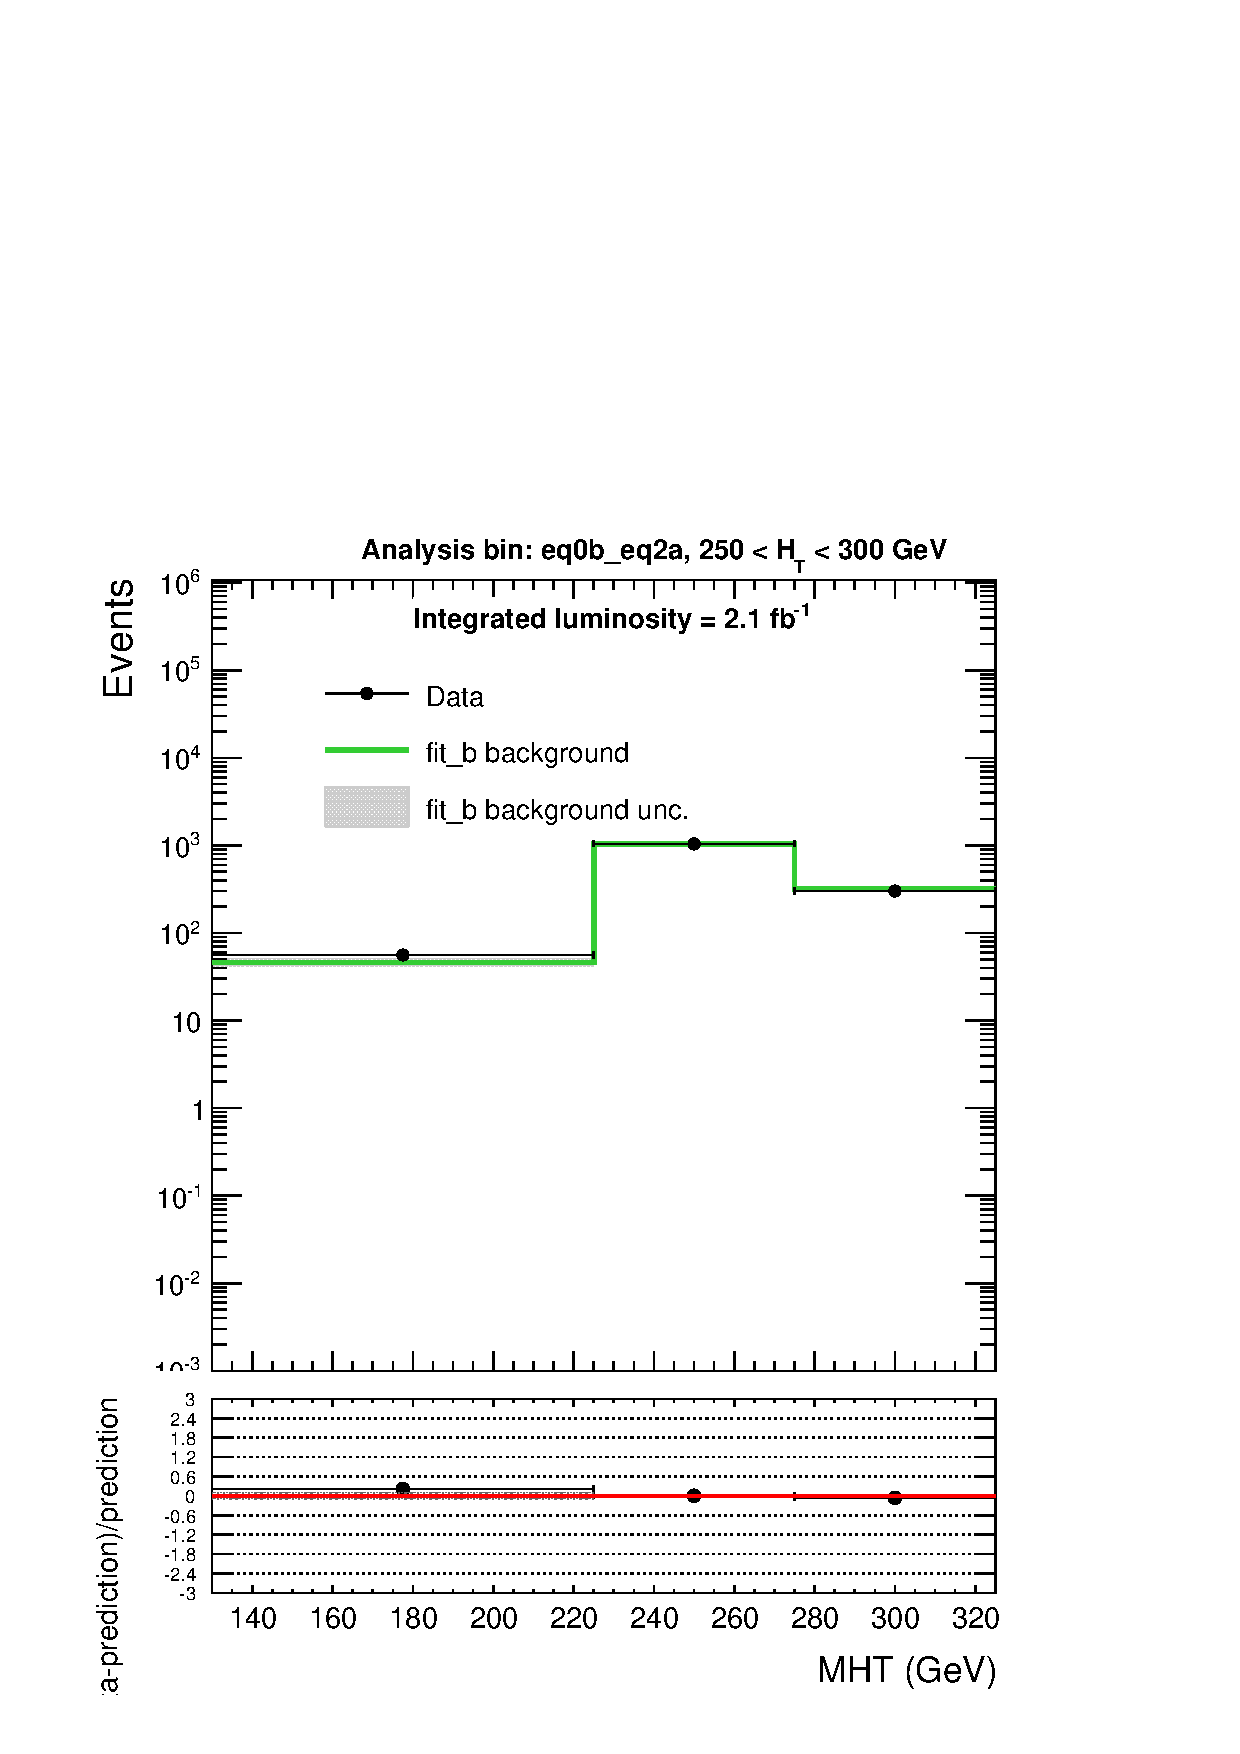
\includegraphics[width=0.25\textwidth]{figures/postFitResults/postFitShapes/postFitShape_eq0b_eq2a_250_300.pdf} }\hspace{1cm}
    \subfigure[$\nj^{\mathrm{asym}}=2$, $\nb=0$, $300 < \scalht < 350 \; \mathrm{GeV}$]{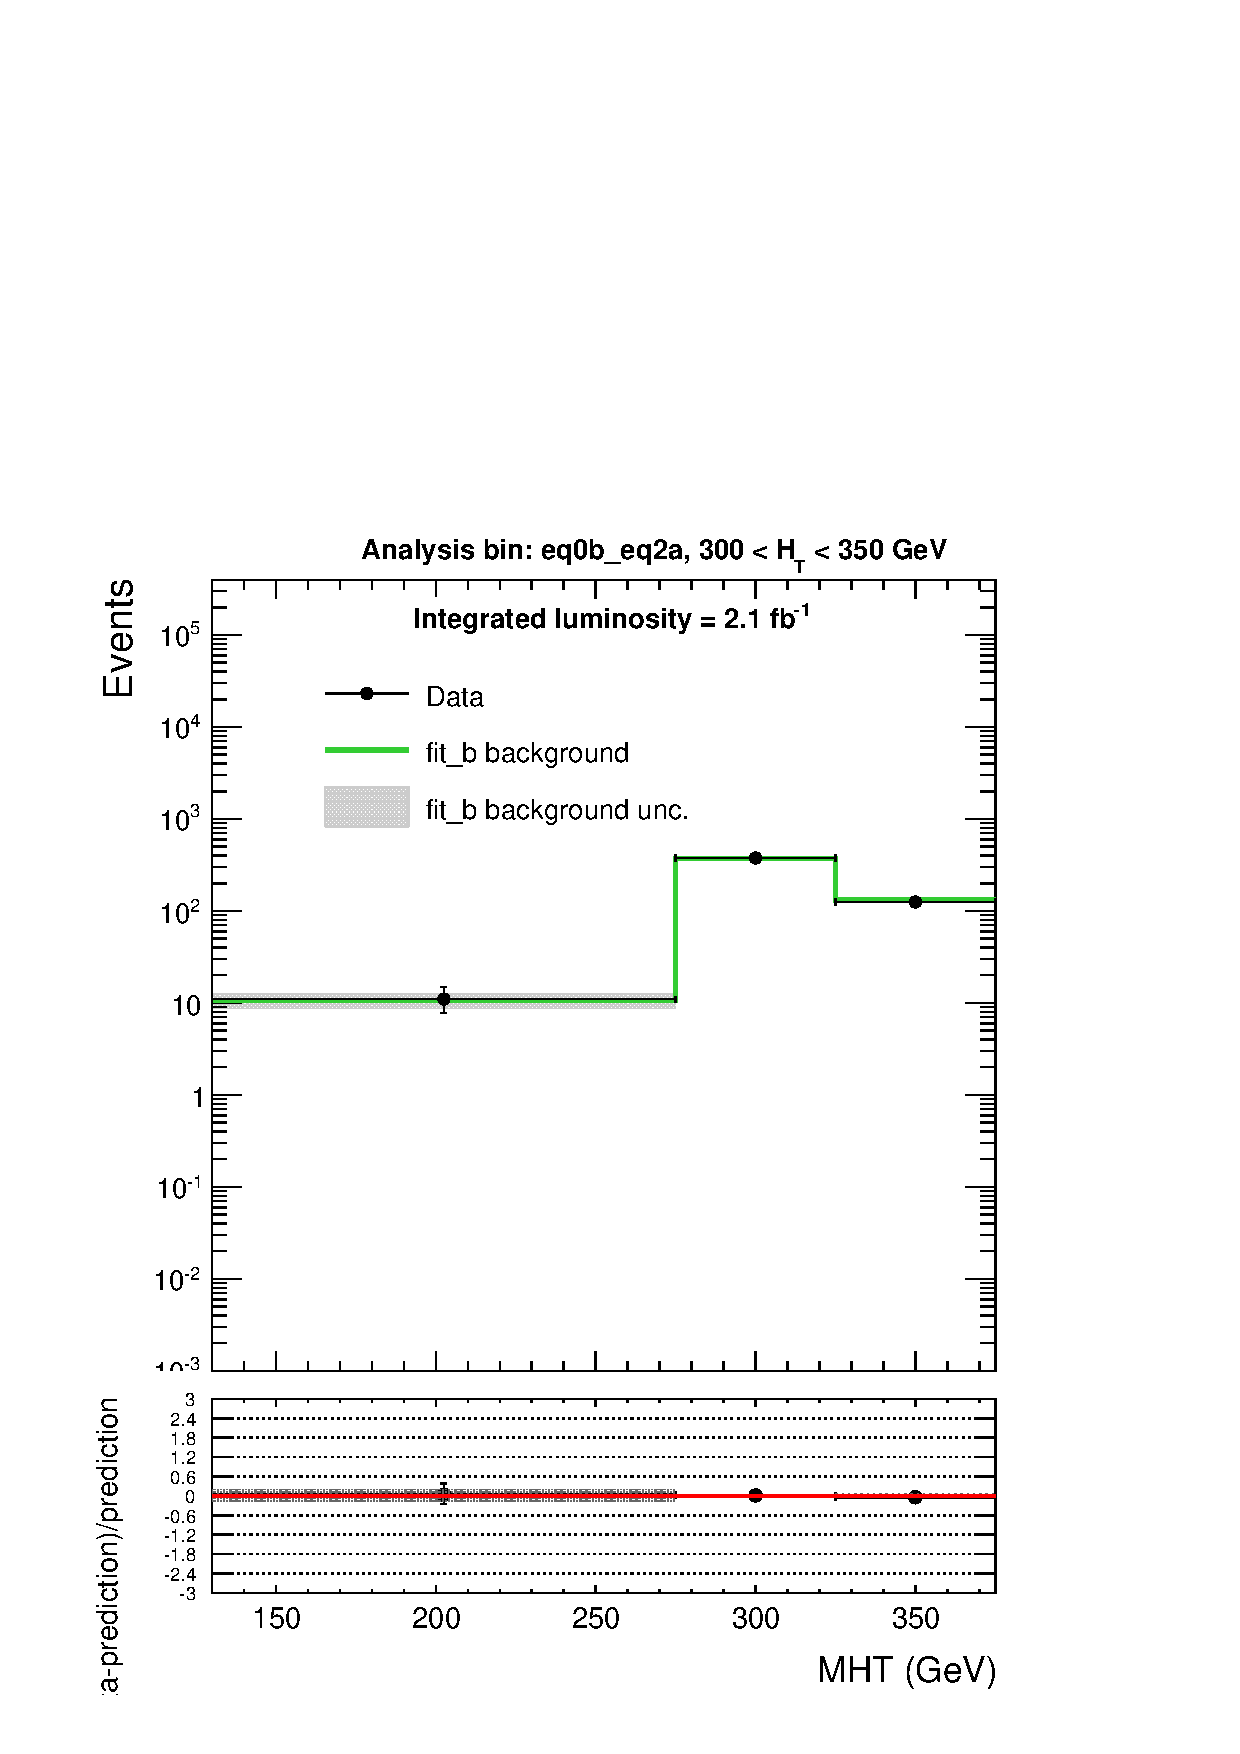
\includegraphics[width=0.25\textwidth]{figures/postFitResults/postFitShapes/postFitShape_eq0b_eq2a_300_350.pdf} }\\
    \subfigure[$\nj^{\mathrm{asym}}=2$, $\nb=0$, $350 < \scalht < 400 \; \mathrm{GeV}$]{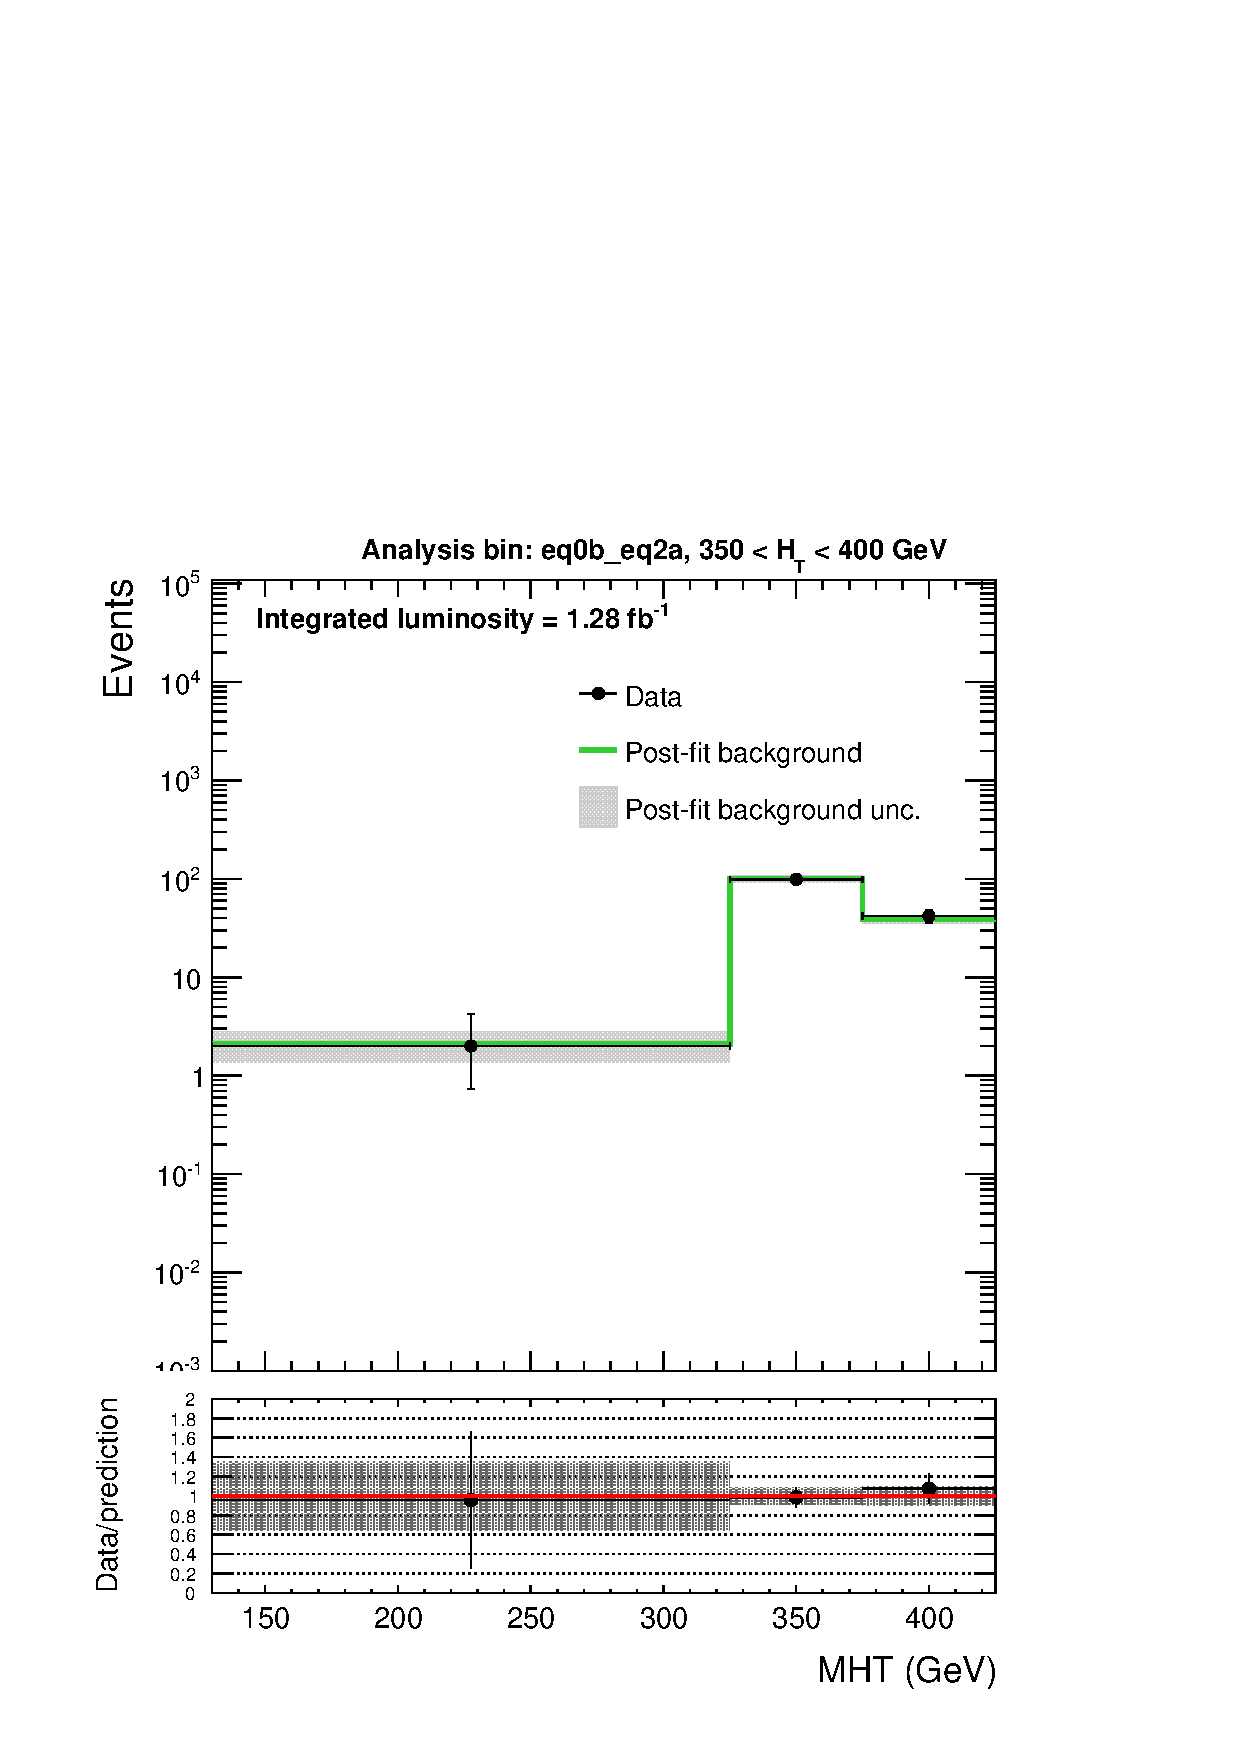
\includegraphics[width=0.25\textwidth]{figures/postFitResults/postFitShapes/postFitShape_eq0b_eq2a_350_400.pdf} }\hspace{1cm}
    \subfigure[$\nj^{\mathrm{asym}}=2$, $\nb=0$, $400 < \scalht < 500 \; \mathrm{GeV}$]{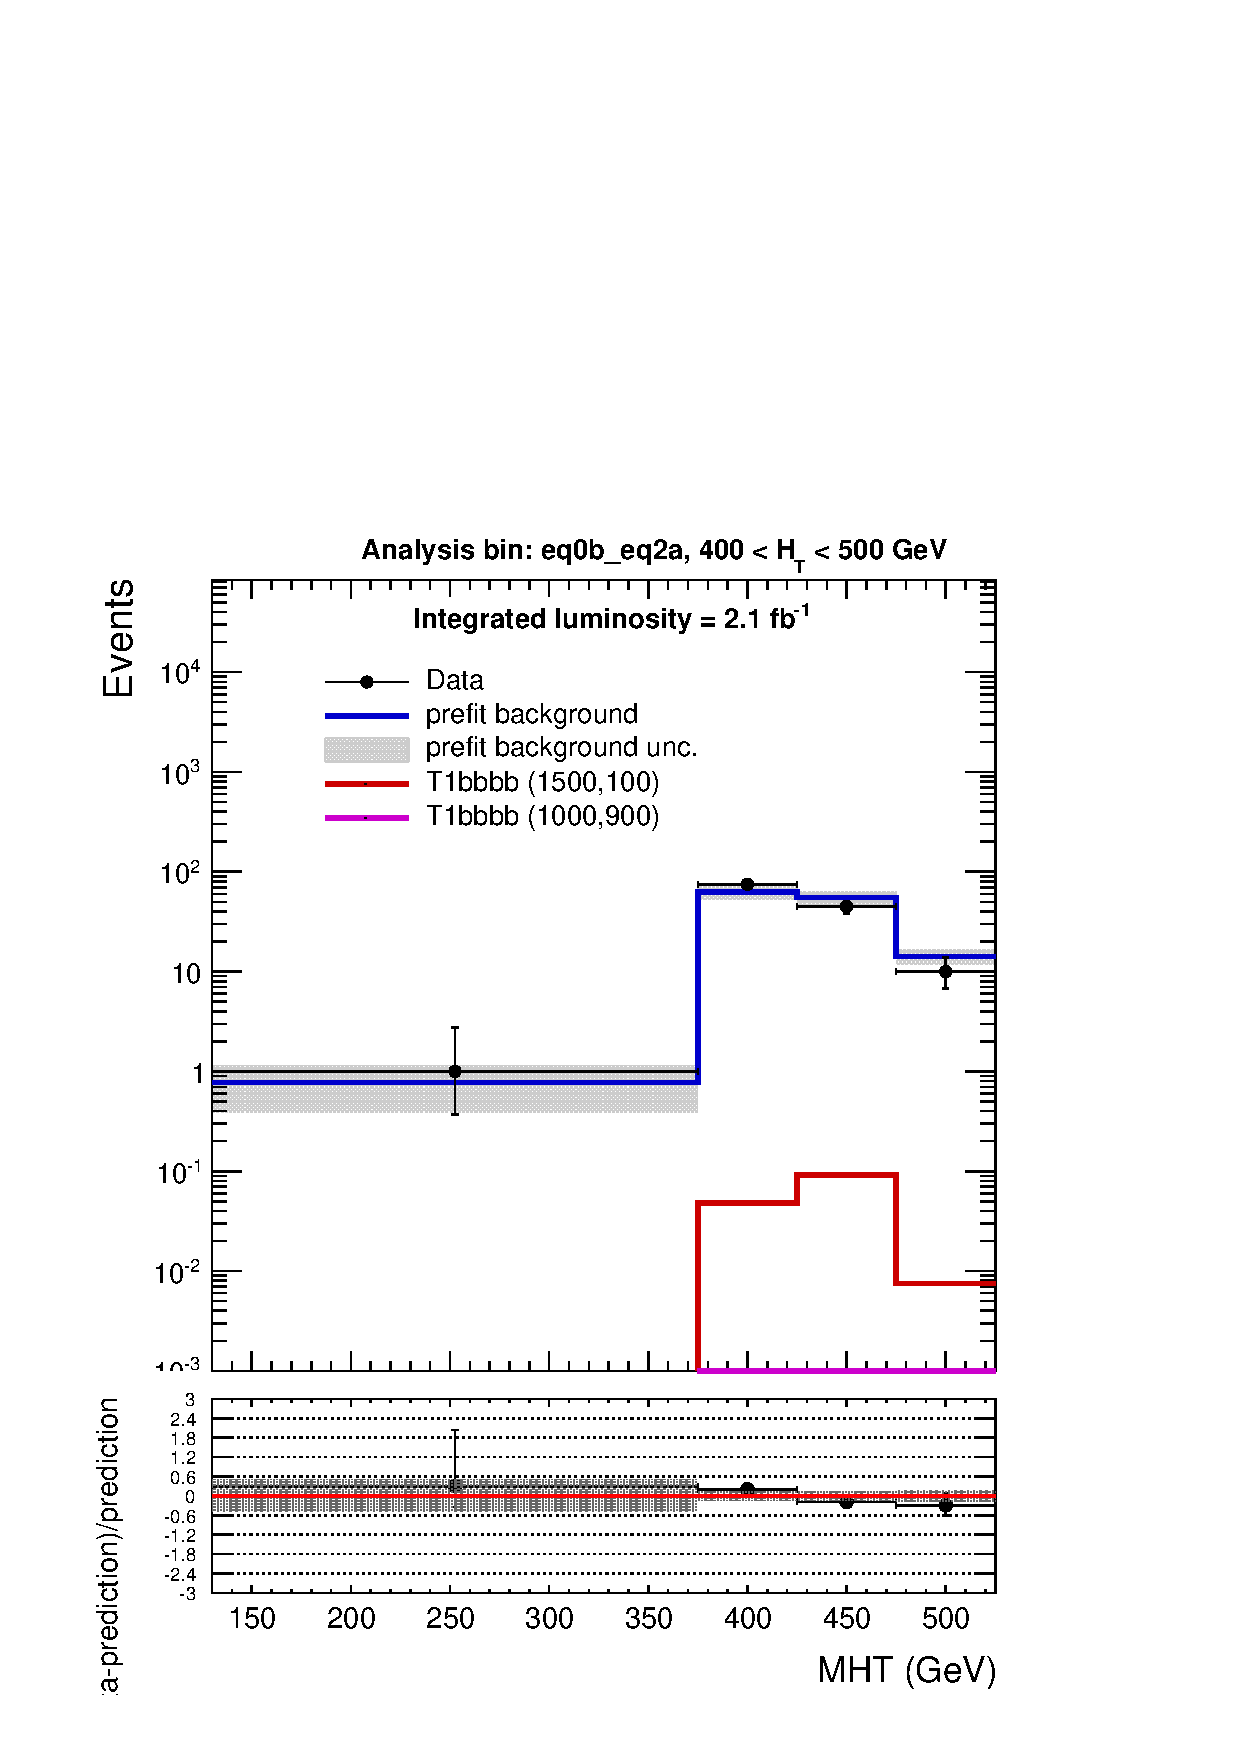
\includegraphics[width=0.25\textwidth]{figures/postFitResults/postFitShapes/postFitShape_eq0b_eq2a_400_500.pdf} }\hspace{1cm}
    \subfigure[$\nj^{\mathrm{asym}}=2$, $\nb=0$, $500 < \scalht < 600 \; \mathrm{GeV}$]{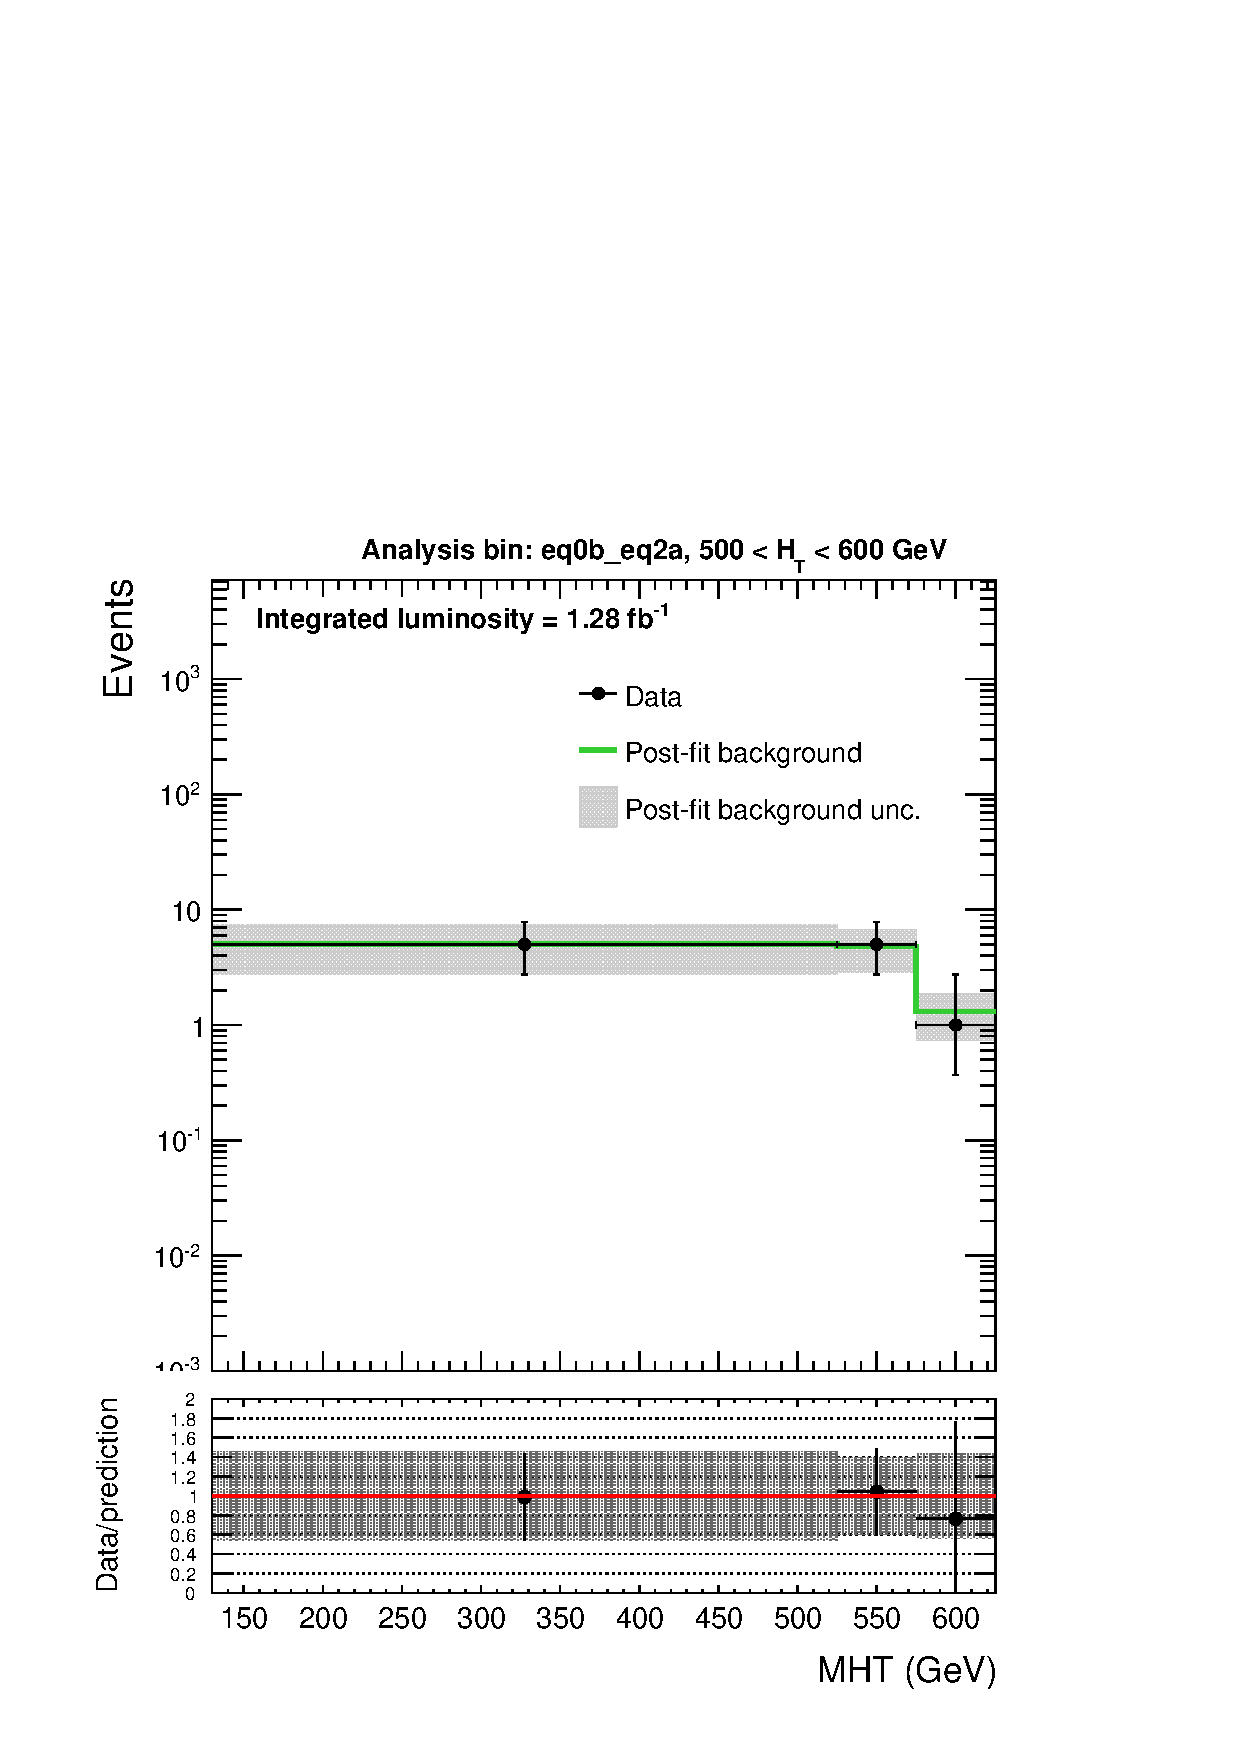
\includegraphics[width=0.25\textwidth]{figures/postFitResults/postFitShapes/postFitShape_eq0b_eq2a_500_600.pdf} }\\
    \subfigure[$\nj^{\mathrm{asym}}=2$, $\nb=0$, $\scalht > 600 \; \mathrm{GeV}$]{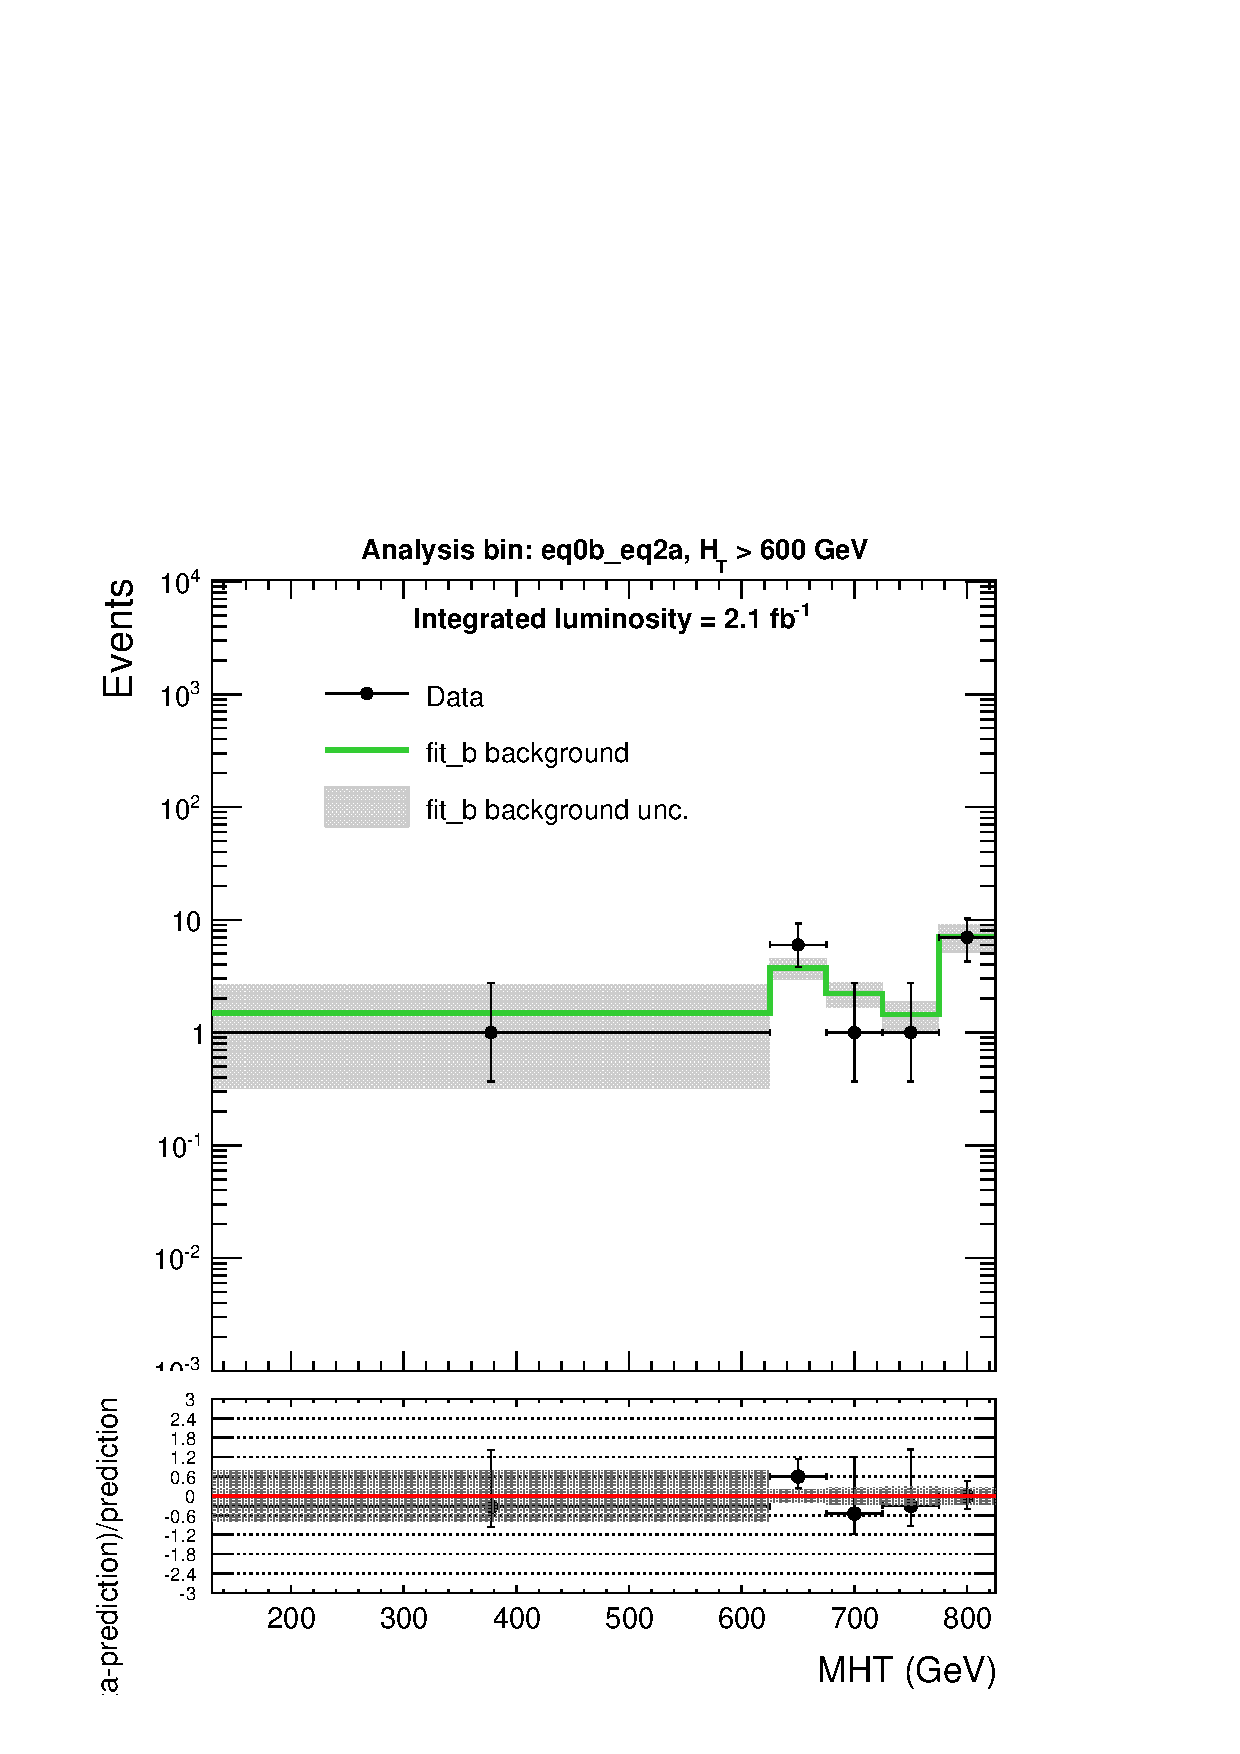
\includegraphics[width=0.25\textwidth]{figures/postFitResults/postFitShapes/postFitShape_eq0b_eq2a_600_Inf.pdf} }\hspace{1cm}
  \end{center}
\end{figure}



\newpage
\begin{figure}[h!]
\caption{Post-fit \MHT templates for the bin $\nj^{\mathrm{sym}}=2$, $\nb=0$ \label{fig:postFitShapes_eq0b_eq2j}}.
\begin{center}

    \subfigure[$\nj^{\mathrm{sym}}=2$, $\nb=0$, $200 < \scalht < 250 \; \mathrm{GeV}$]{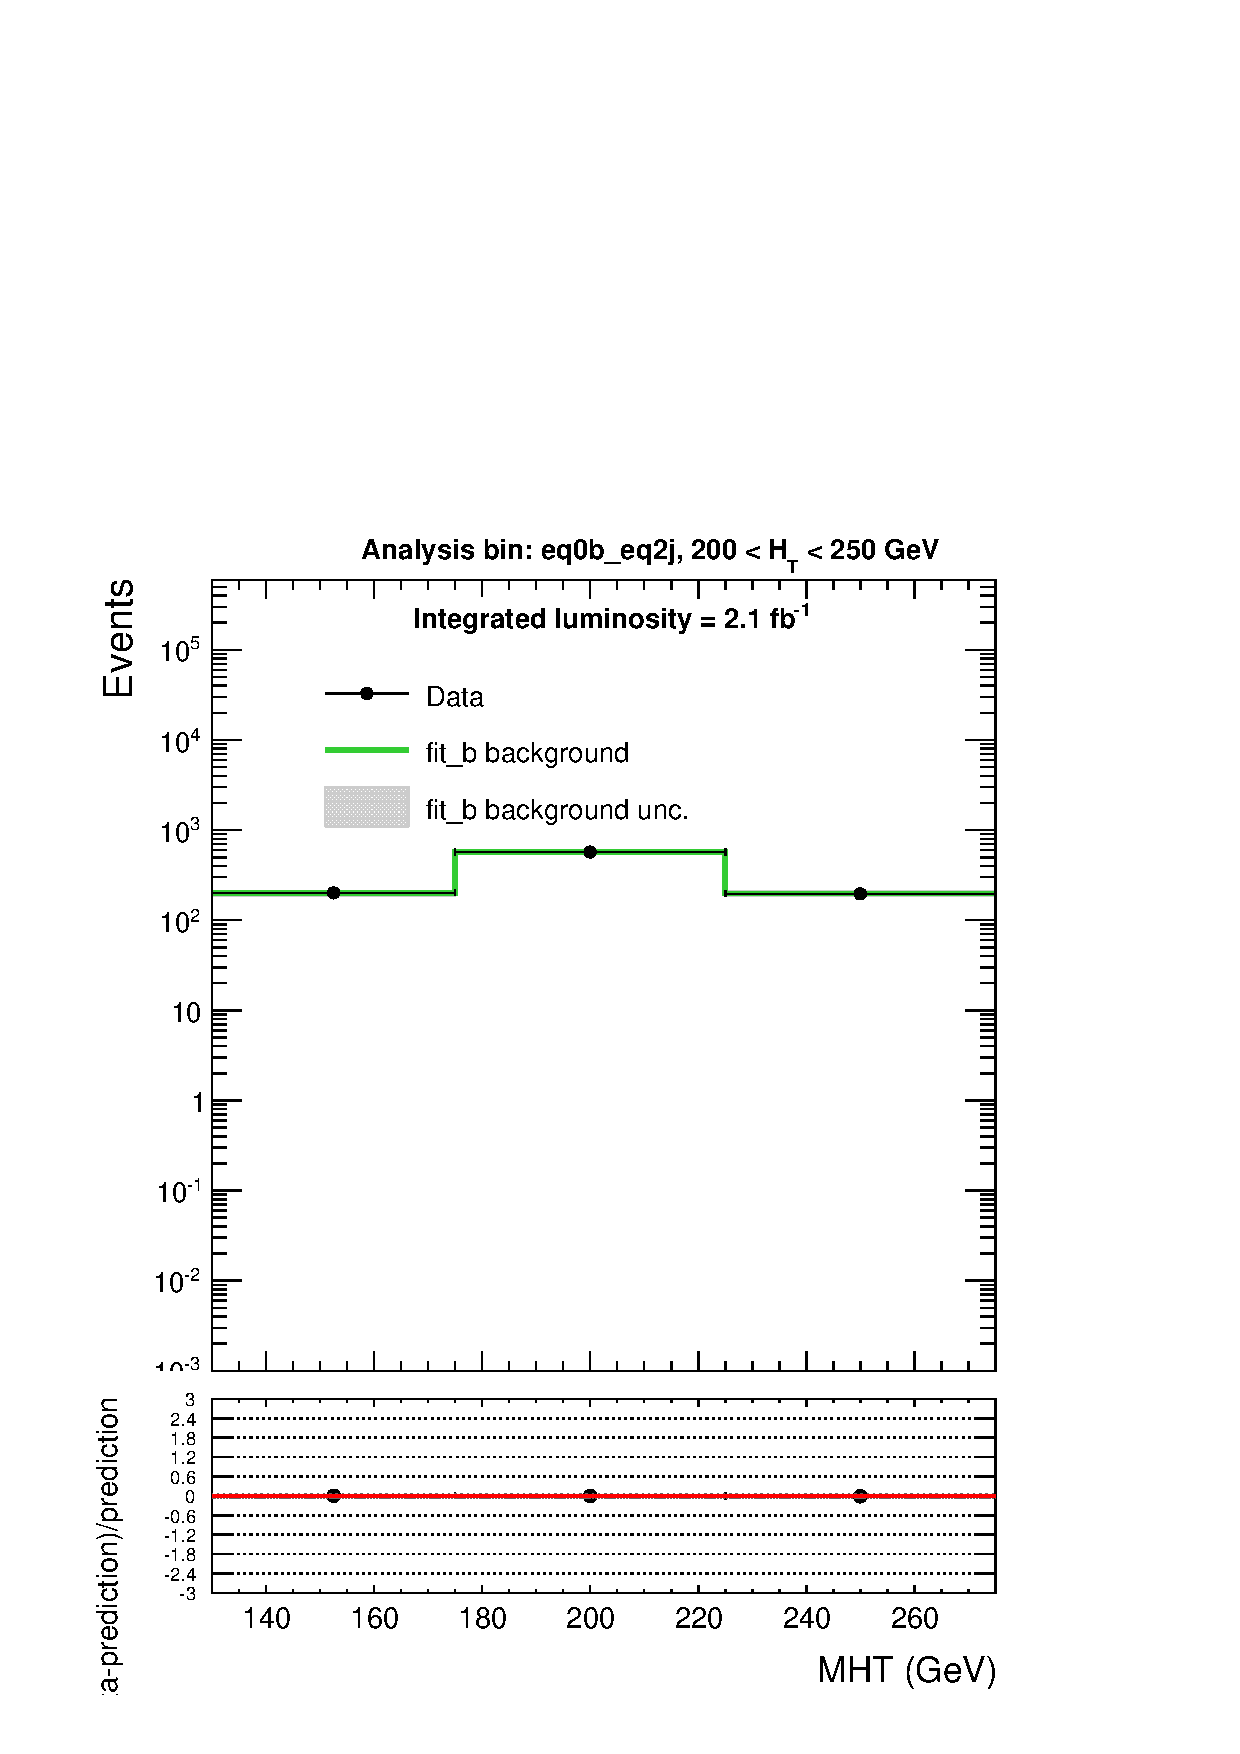
\includegraphics[width=0.25\textwidth]{figures/postFitResults/postFitShapes/postFitShape_eq0b_eq2j_200_250.pdf} }\hspace{1cm}
    \subfigure[$\nj^{\mathrm{sym}}=2$, $\nb=0$, $250 < \scalht < 300 \; \mathrm{GeV}$]{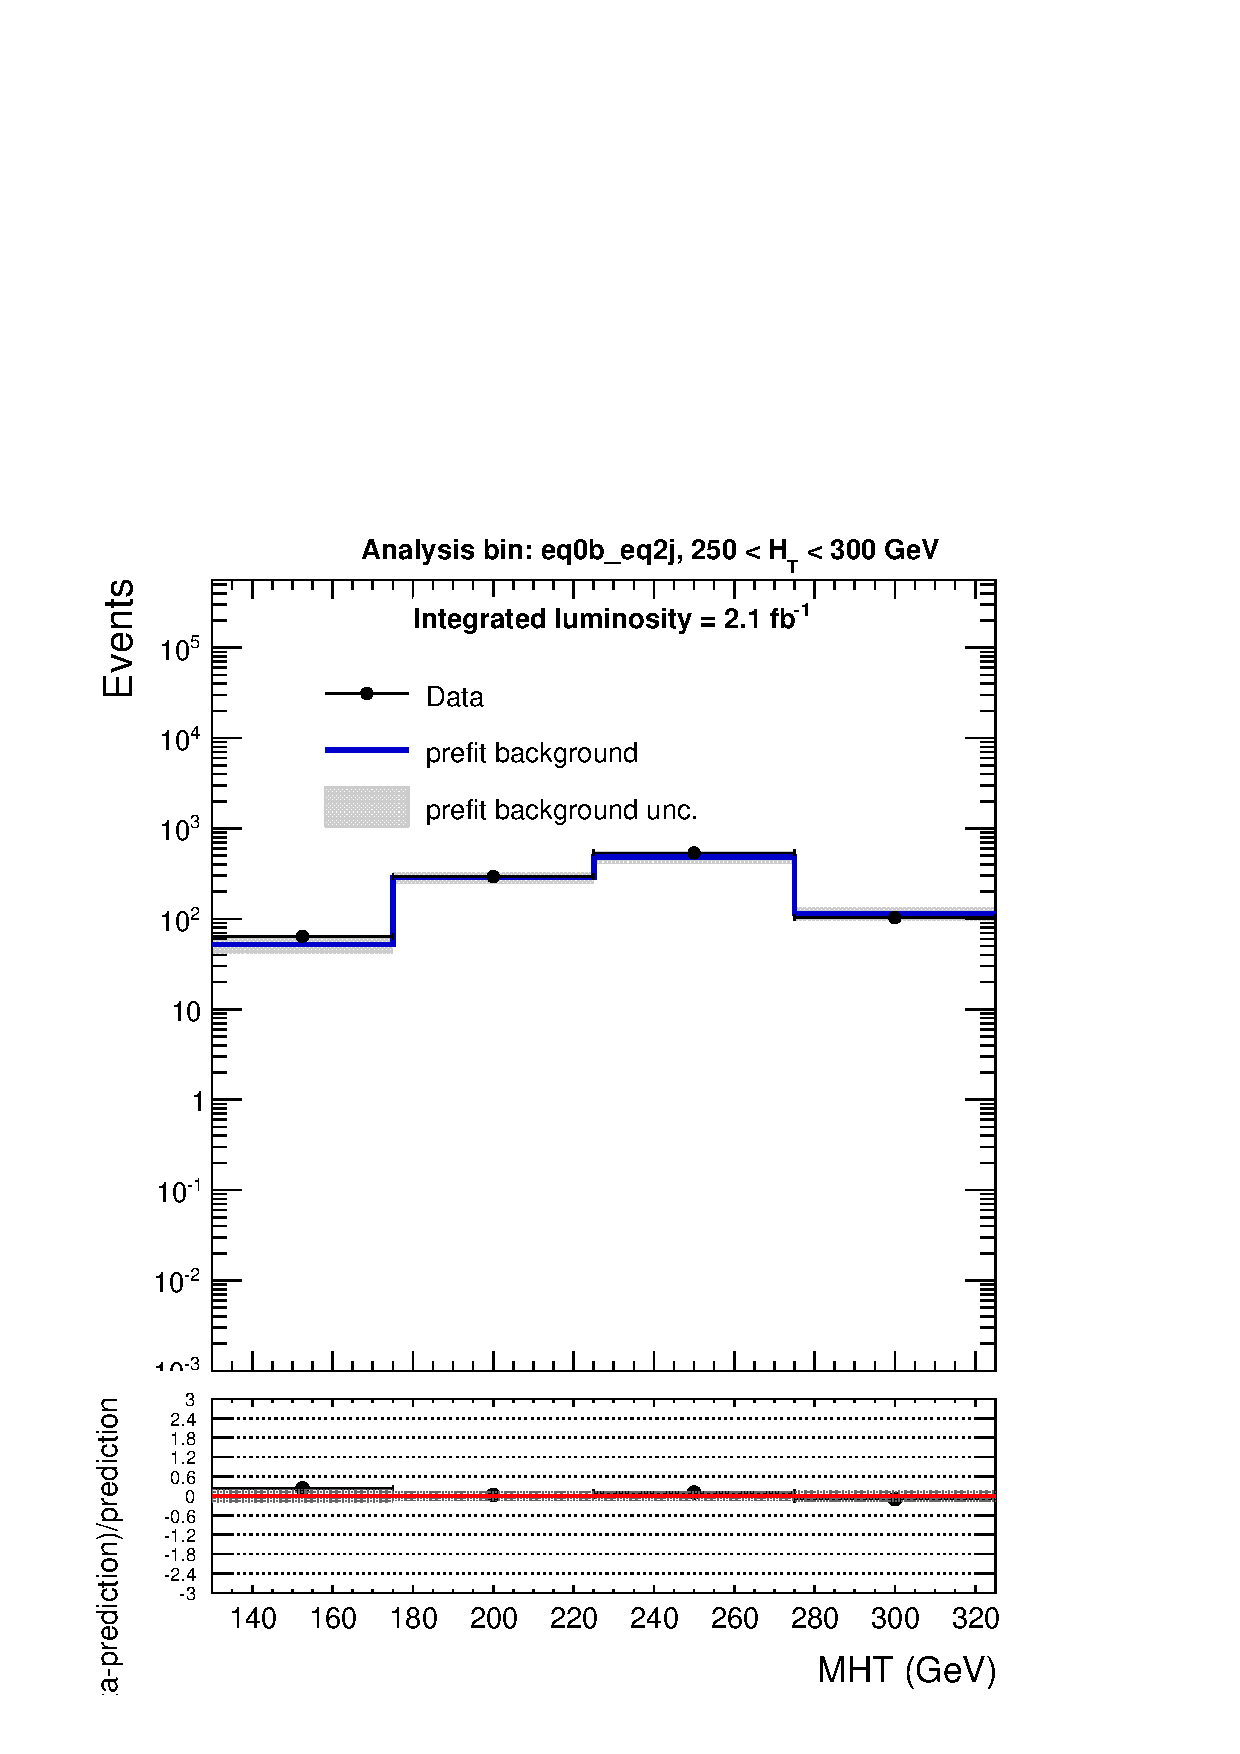
\includegraphics[width=0.25\textwidth]{figures/postFitResults/postFitShapes/postFitShape_eq0b_eq2j_250_300.pdf} }\hspace{1cm}
    \subfigure[$\nj^{\mathrm{sym}}=2$, $\nb=0$, $300 < \scalht < 350 \; \mathrm{GeV}$]{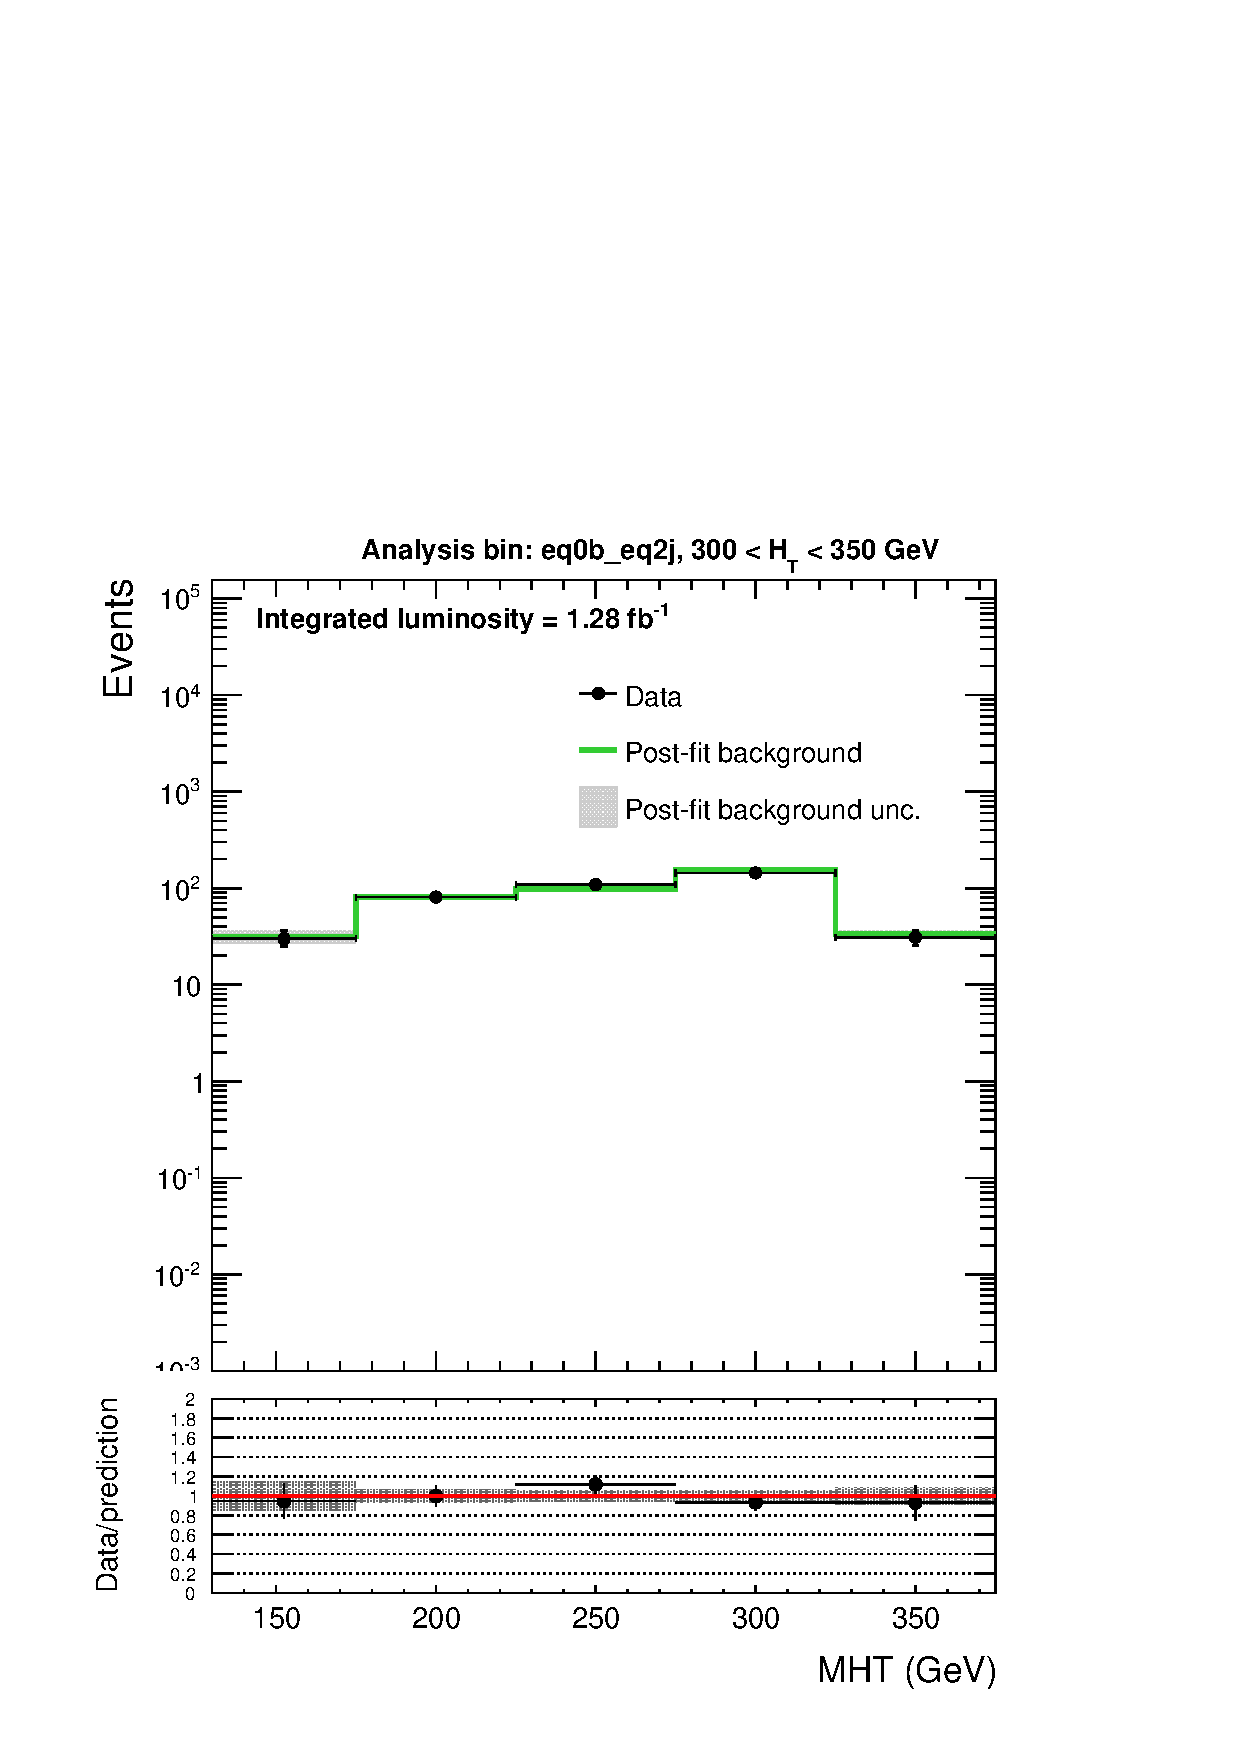
\includegraphics[width=0.25\textwidth]{figures/postFitResults/postFitShapes/postFitShape_eq0b_eq2j_300_350.pdf} }\\
    \subfigure[$\nj^{\mathrm{sym}}=2$, $\nb=0$, $350 < \scalht < 400 \; \mathrm{GeV}$]{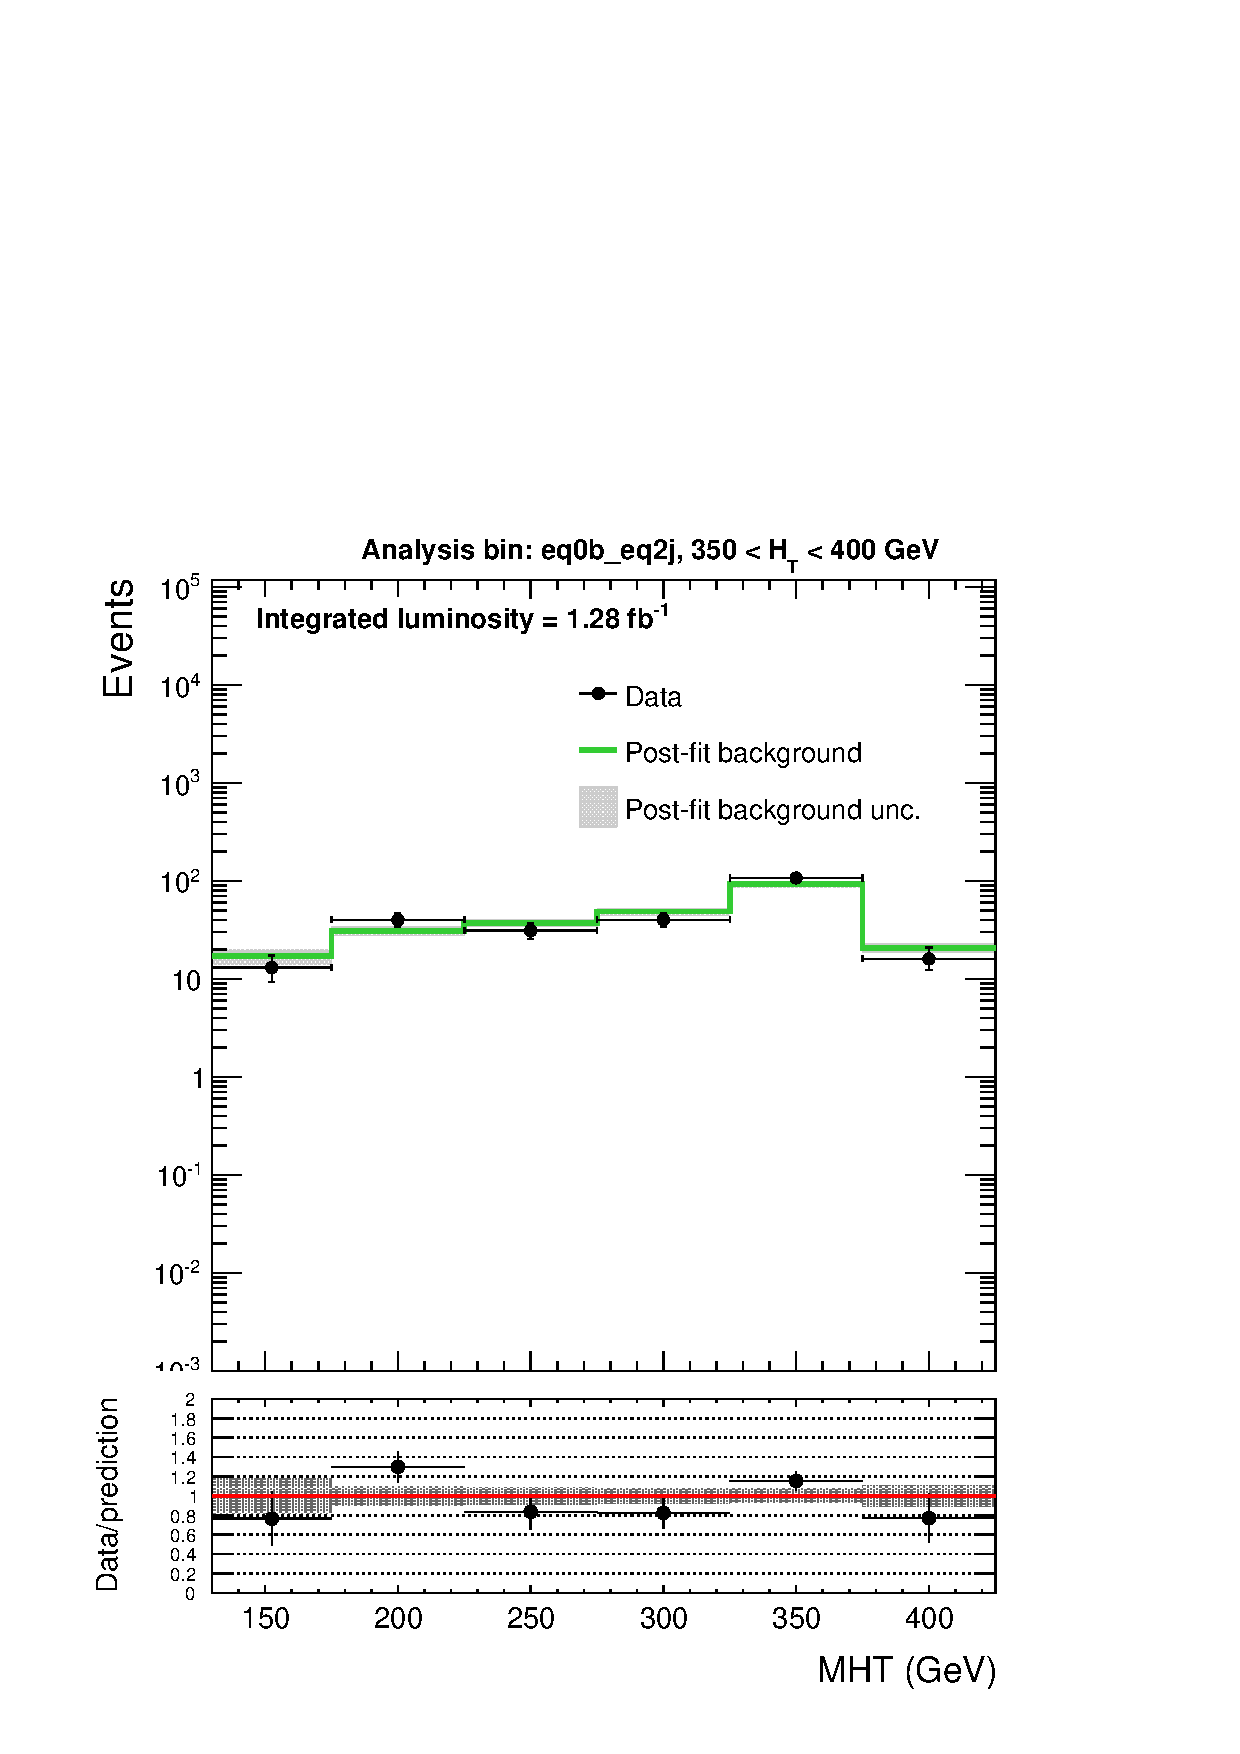
\includegraphics[width=0.25\textwidth]{figures/postFitResults/postFitShapes/postFitShape_eq0b_eq2j_350_400.pdf} }\hspace{1cm}
    \subfigure[$\nj^{\mathrm{sym}}=2$, $\nb=0$, $400 < \scalht < 500 \; \mathrm{GeV}$]{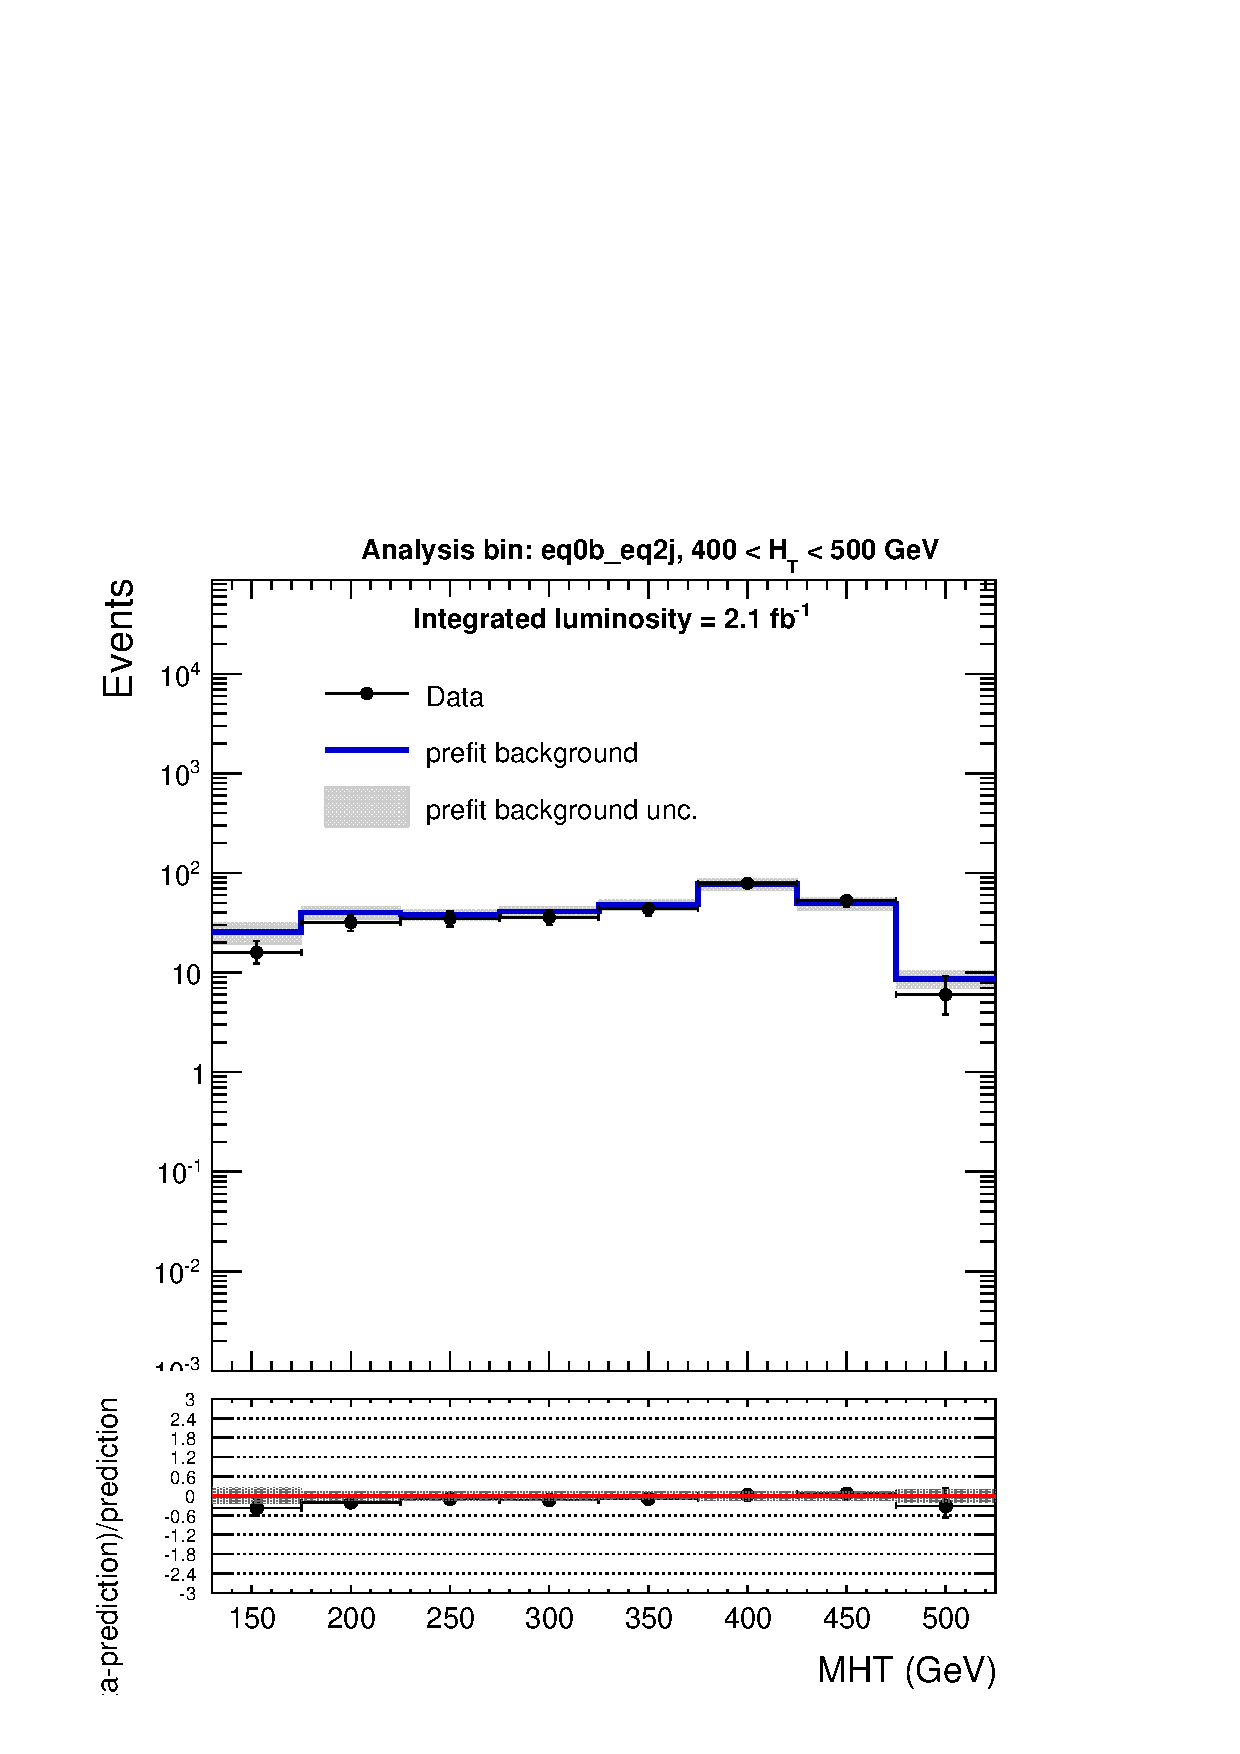
\includegraphics[width=0.25\textwidth]{figures/postFitResults/postFitShapes/postFitShape_eq0b_eq2j_400_500.pdf} }\hspace{1cm}
    \subfigure[$\nj^{\mathrm{sym}}=2$, $\nb=0$, $500 < \scalht < 600 \; \mathrm{GeV}$]{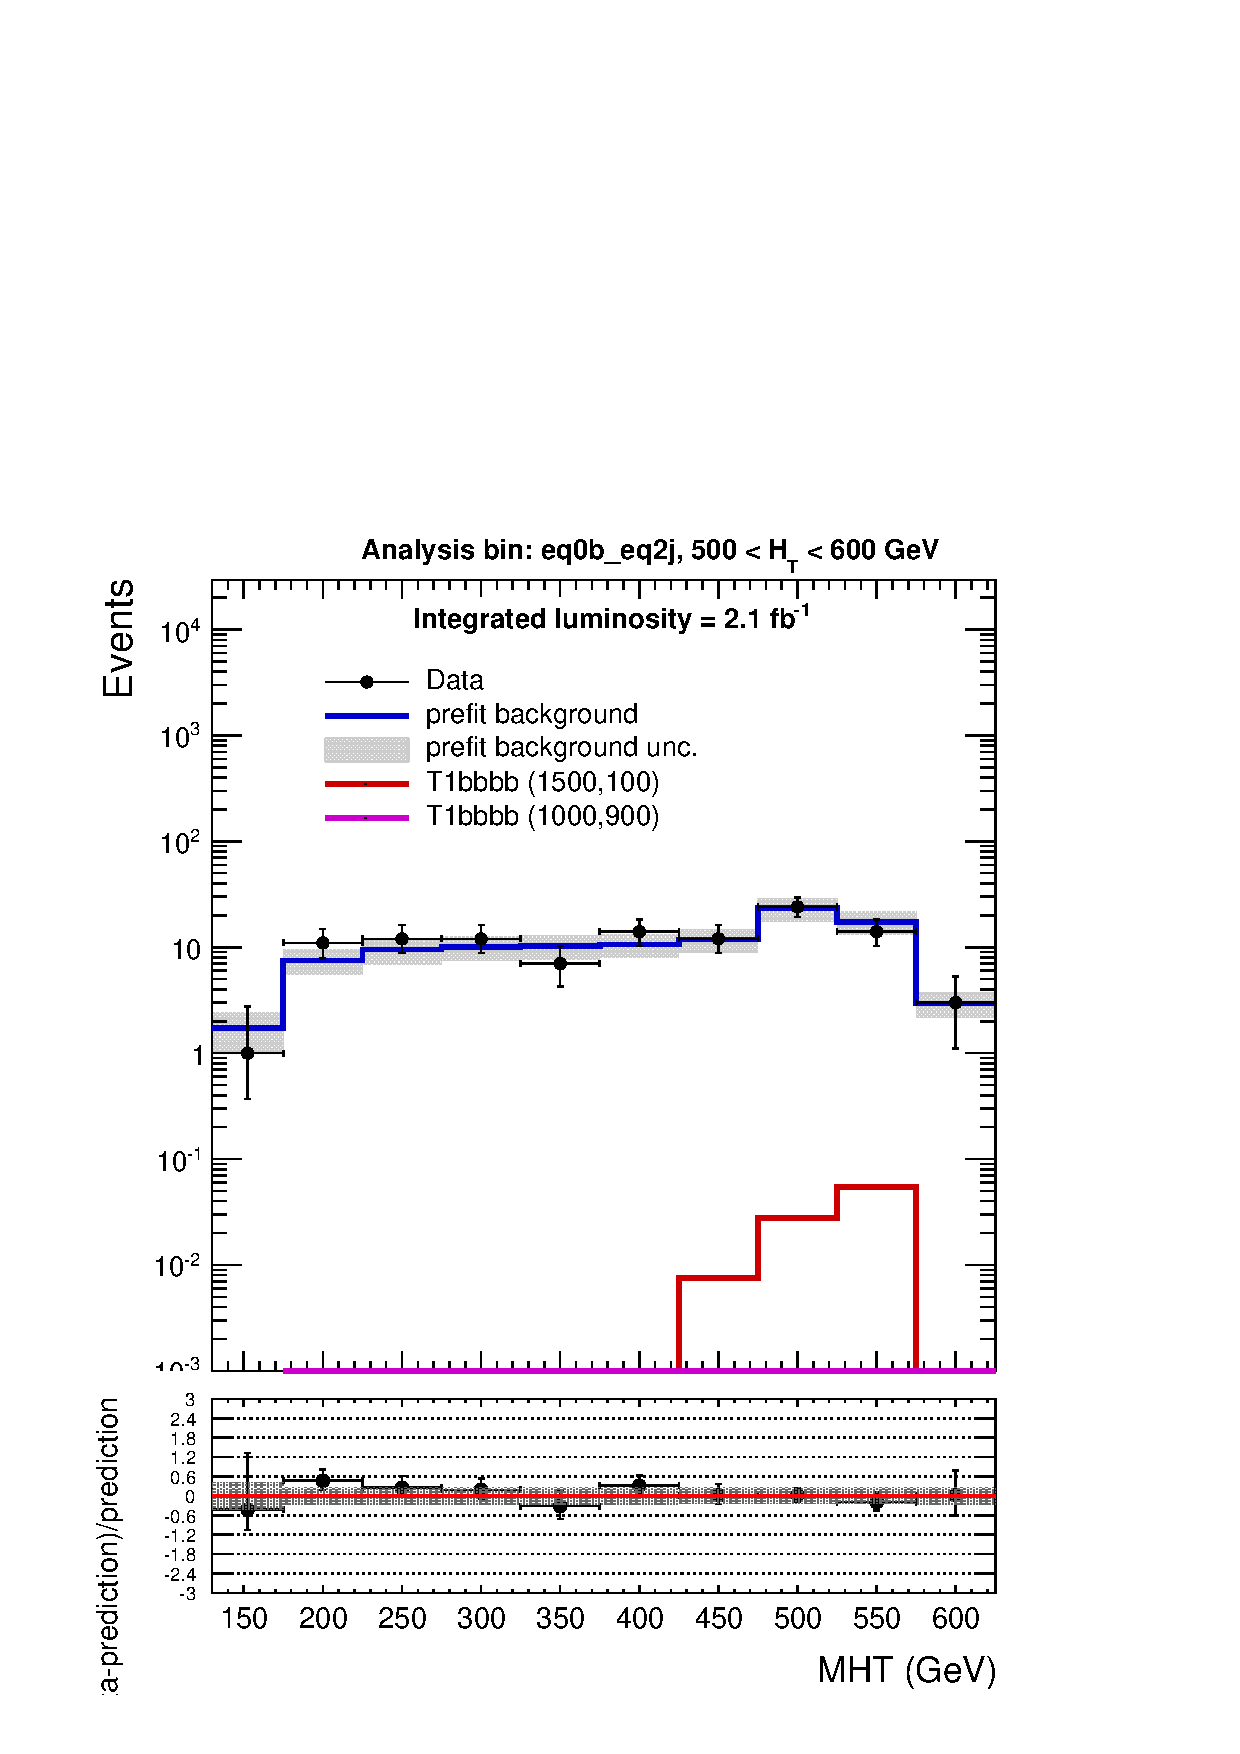
\includegraphics[width=0.25\textwidth]{figures/postFitResults/postFitShapes/postFitShape_eq0b_eq2j_500_600.pdf} }\\
    \subfigure[$\nj^{\mathrm{sym}}=2$, $\nb=0$, $600 < \scalht < 800 \; \mathrm{GeV}$]{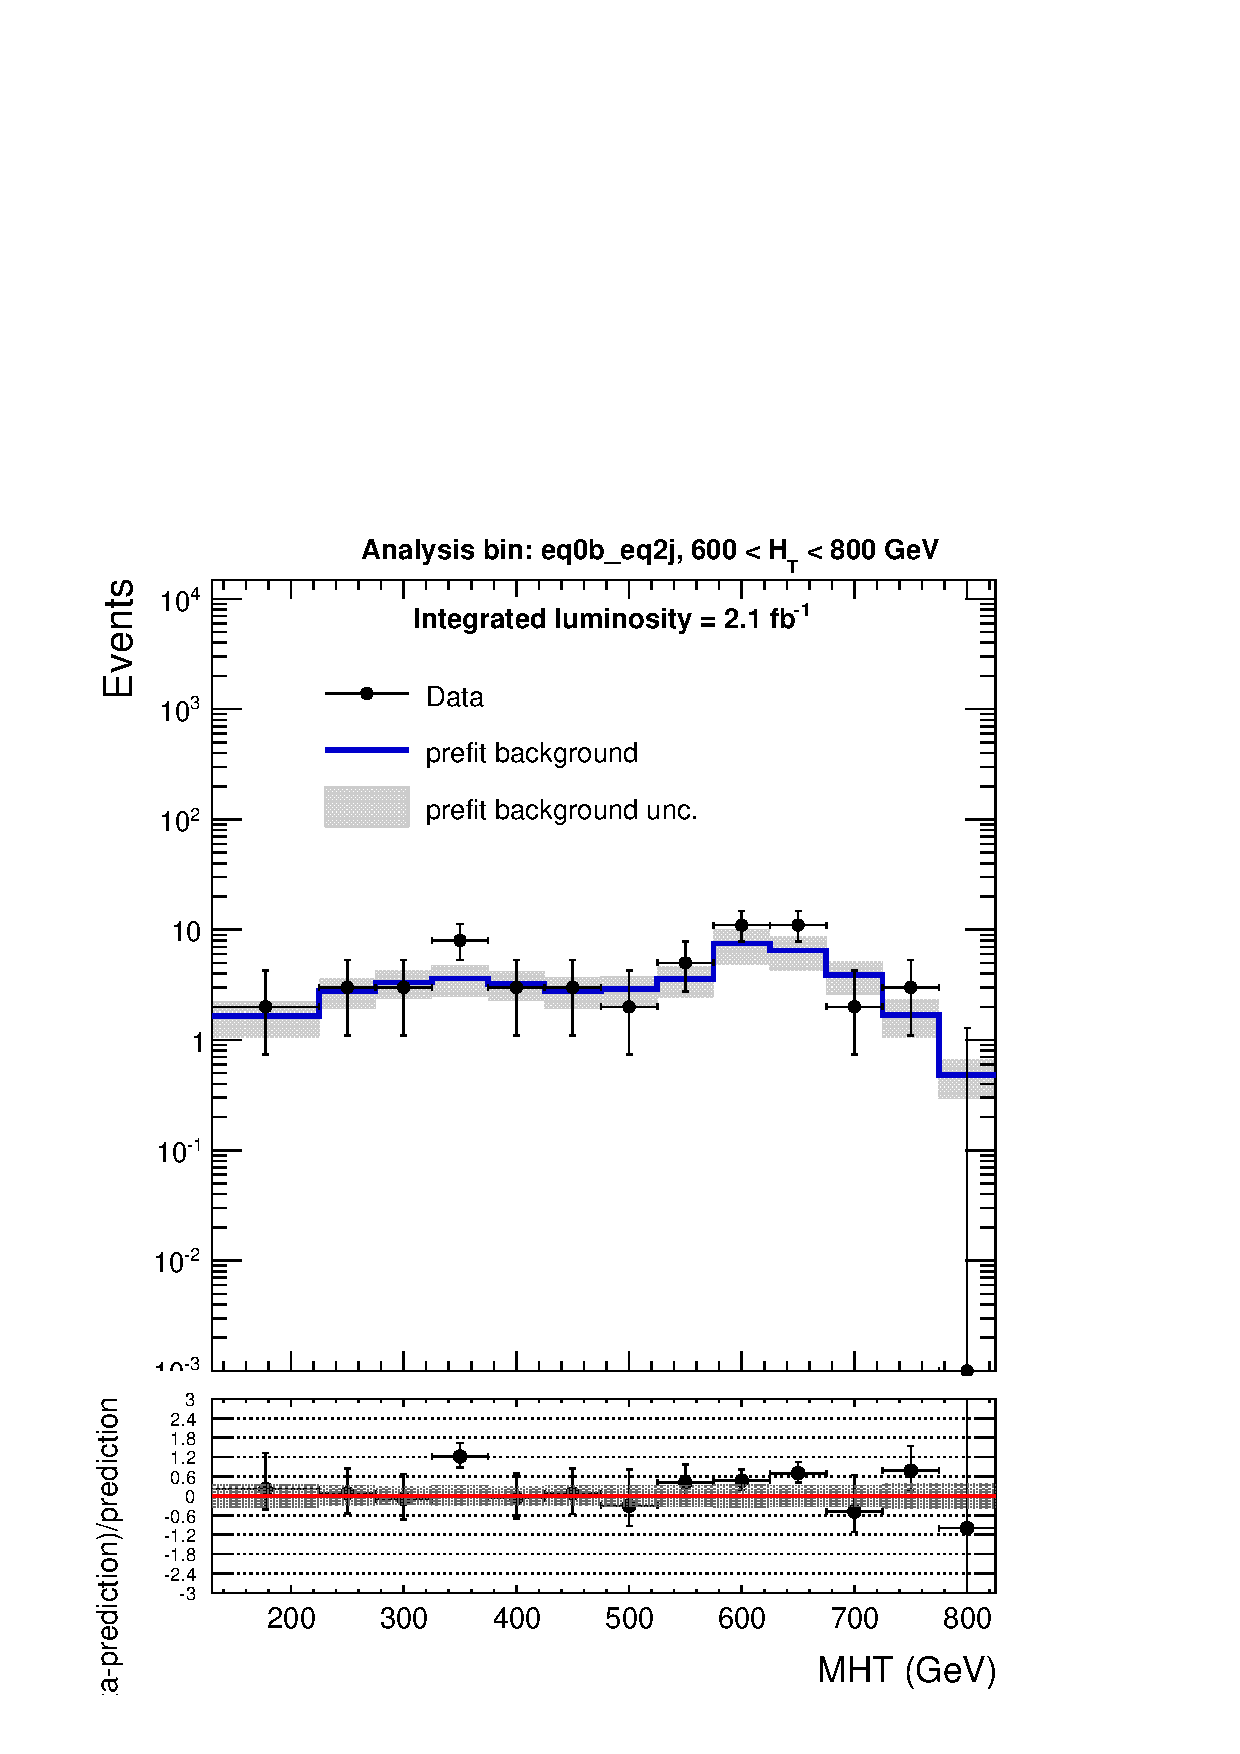
\includegraphics[width=0.25\textwidth]{figures/postFitResults/postFitShapes/postFitShape_eq0b_eq2j_600_800.pdf} }\hspace{1cm}
    \subfigure[$\nj^{\mathrm{sym}}=2$, $\nb=0$, $\scalht > 800 \; \mathrm{GeV}$]{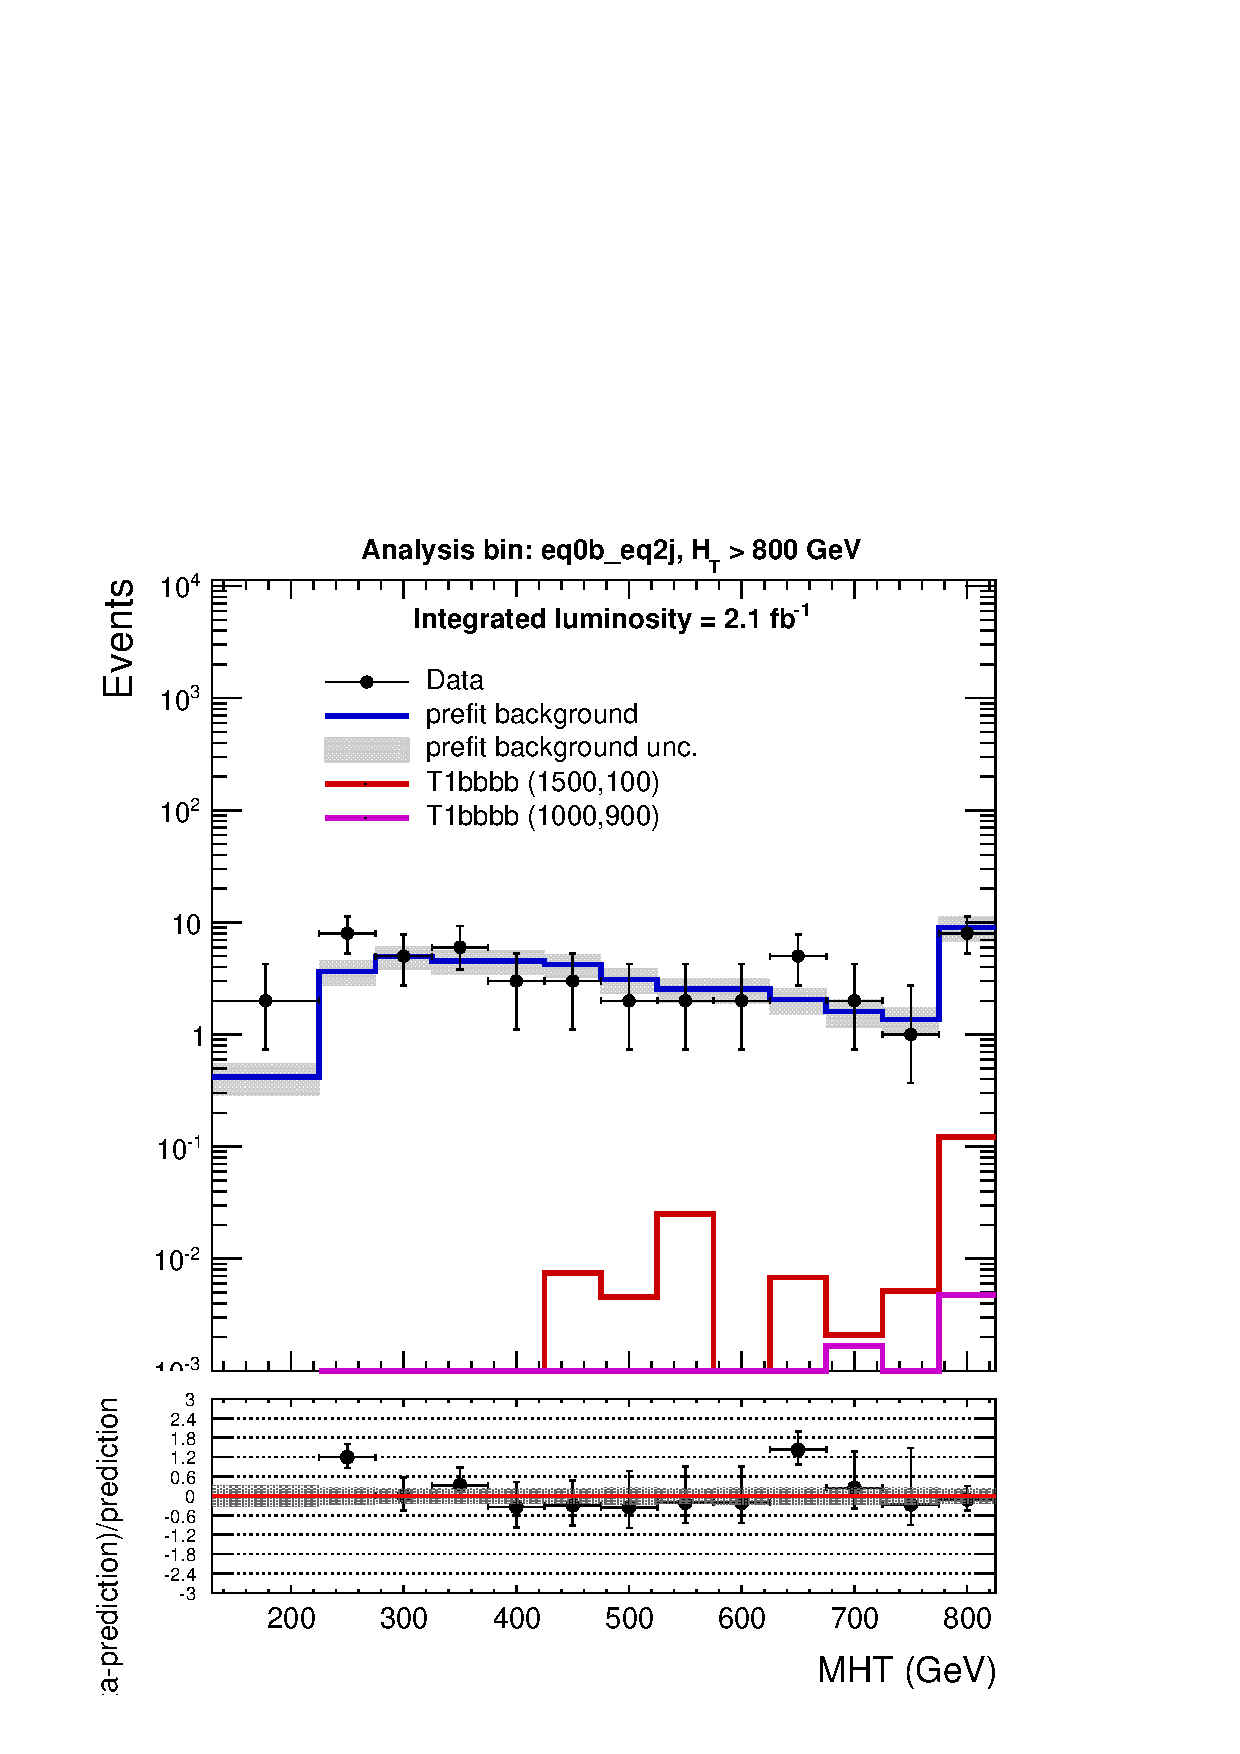
\includegraphics[width=0.25\textwidth]{figures/postFitResults/postFitShapes/postFitShape_eq0b_eq2j_800_Inf.pdf} }\hspace{1cm}
  \end{center}
\end{figure}



\newpage
\begin{figure}[h!]
\caption{Post-fit \MHT templates for the bin $\nj^{\mathrm{asym}}=3$, $\nb=0$ \label{fig:postFitShapes_eq0b_eq3a}}.
\begin{center}

    \subfigure[$\nj^{\mathrm{asym}}=3$, $\nb=0$, $200 < \scalht < 250 \; \mathrm{GeV}$]{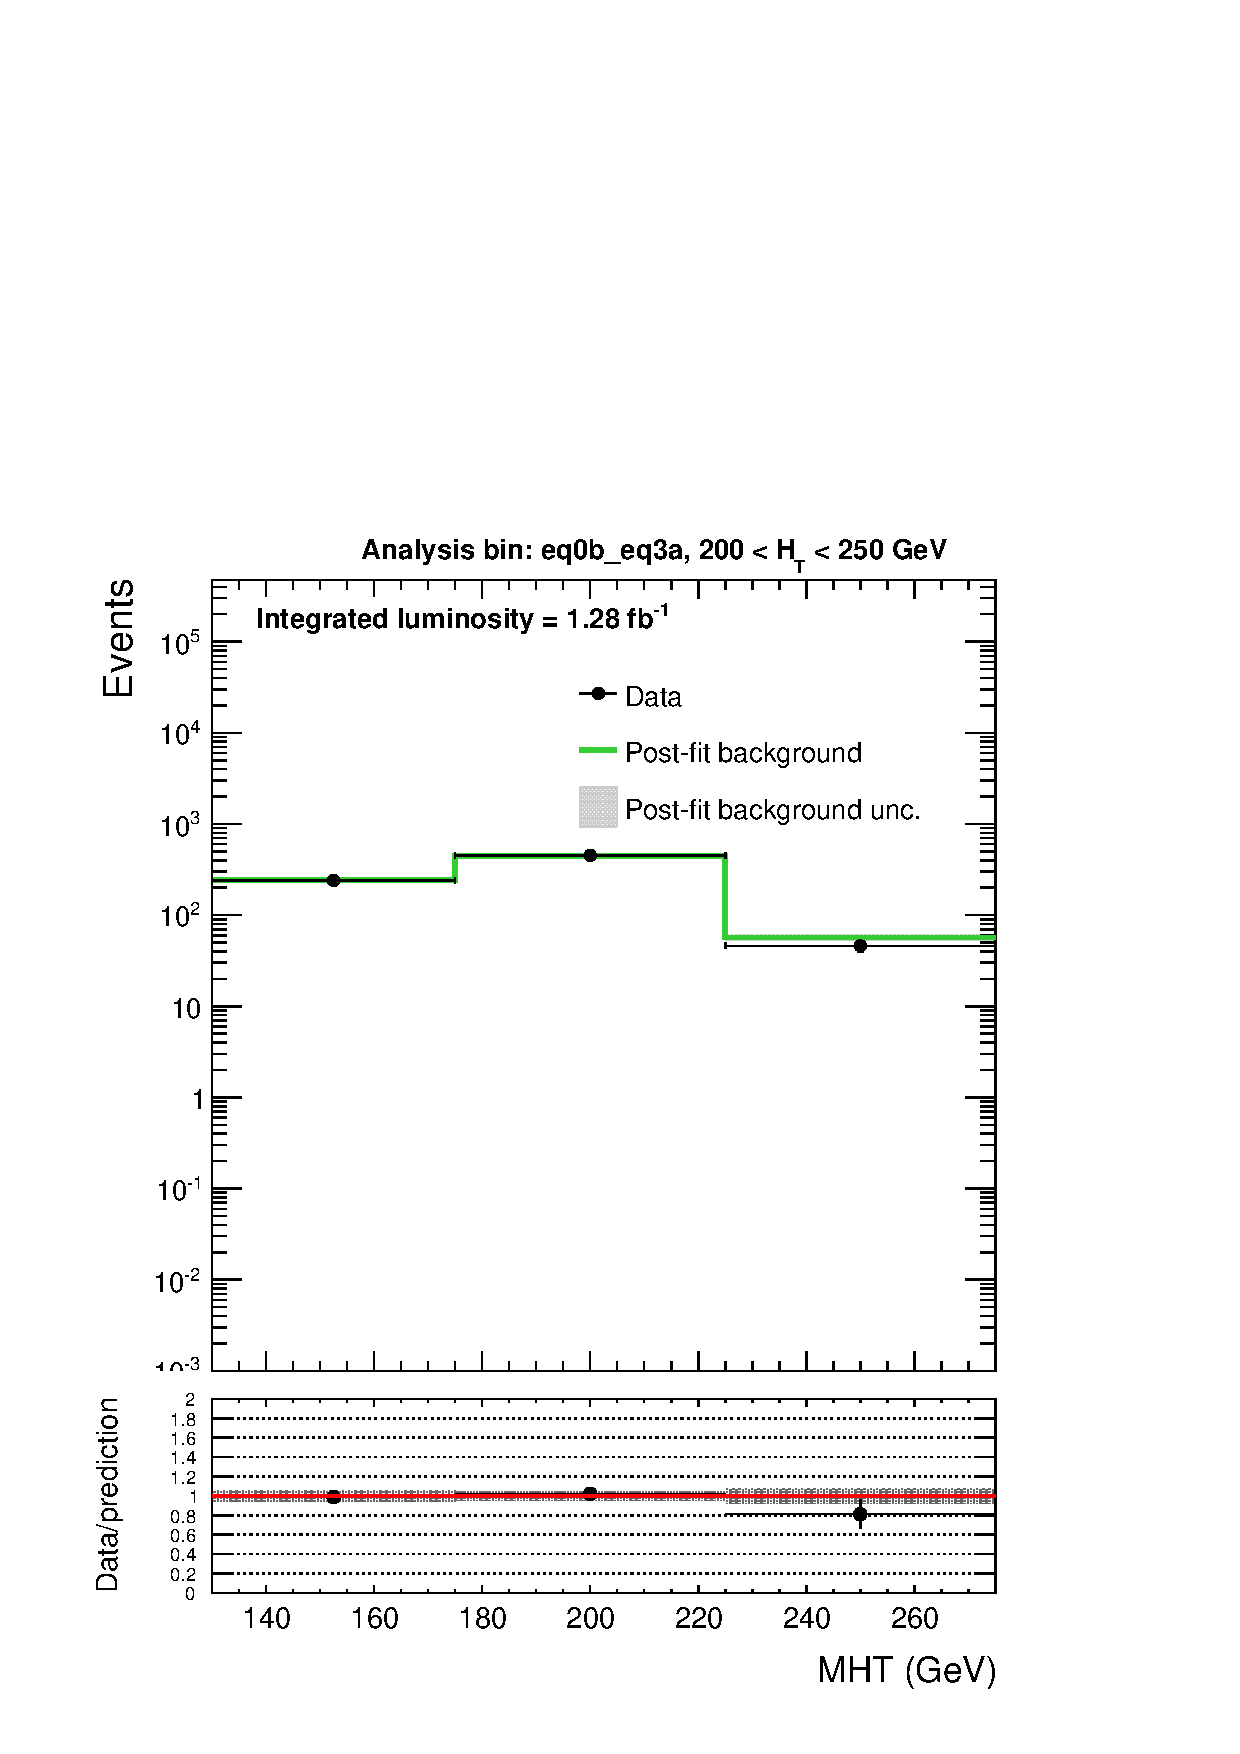
\includegraphics[width=0.25\textwidth]{figures/postFitResults/postFitShapes/postFitShape_eq0b_eq3a_200_250.pdf} }\hspace{1cm}
    \subfigure[$\nj^{\mathrm{asym}}=3$, $\nb=0$, $250 < \scalht < 300 \; \mathrm{GeV}$]{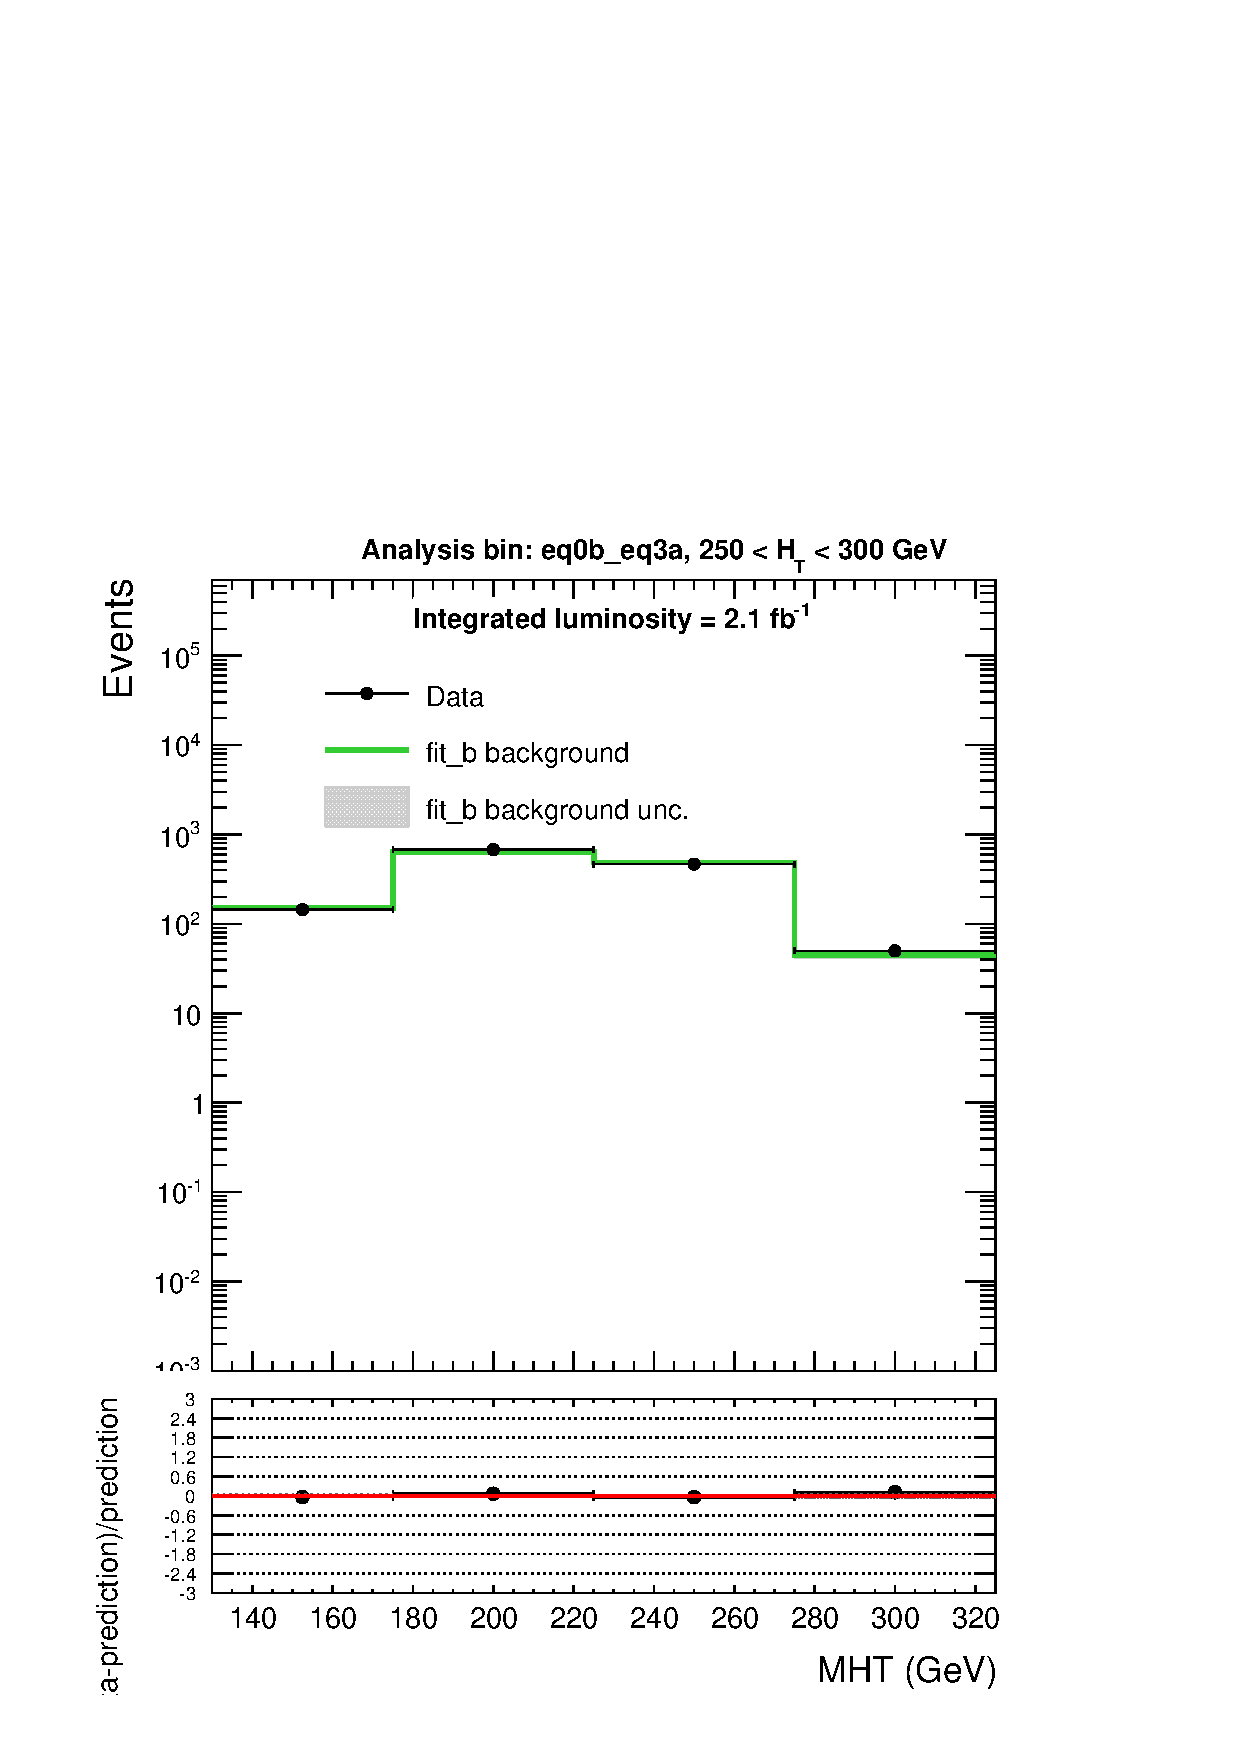
\includegraphics[width=0.25\textwidth]{figures/postFitResults/postFitShapes/postFitShape_eq0b_eq3a_250_300.pdf} }\hspace{1cm}
    \subfigure[$\nj^{\mathrm{asym}}=3$, $\nb=0$, $300 < \scalht < 350 \; \mathrm{GeV}$]{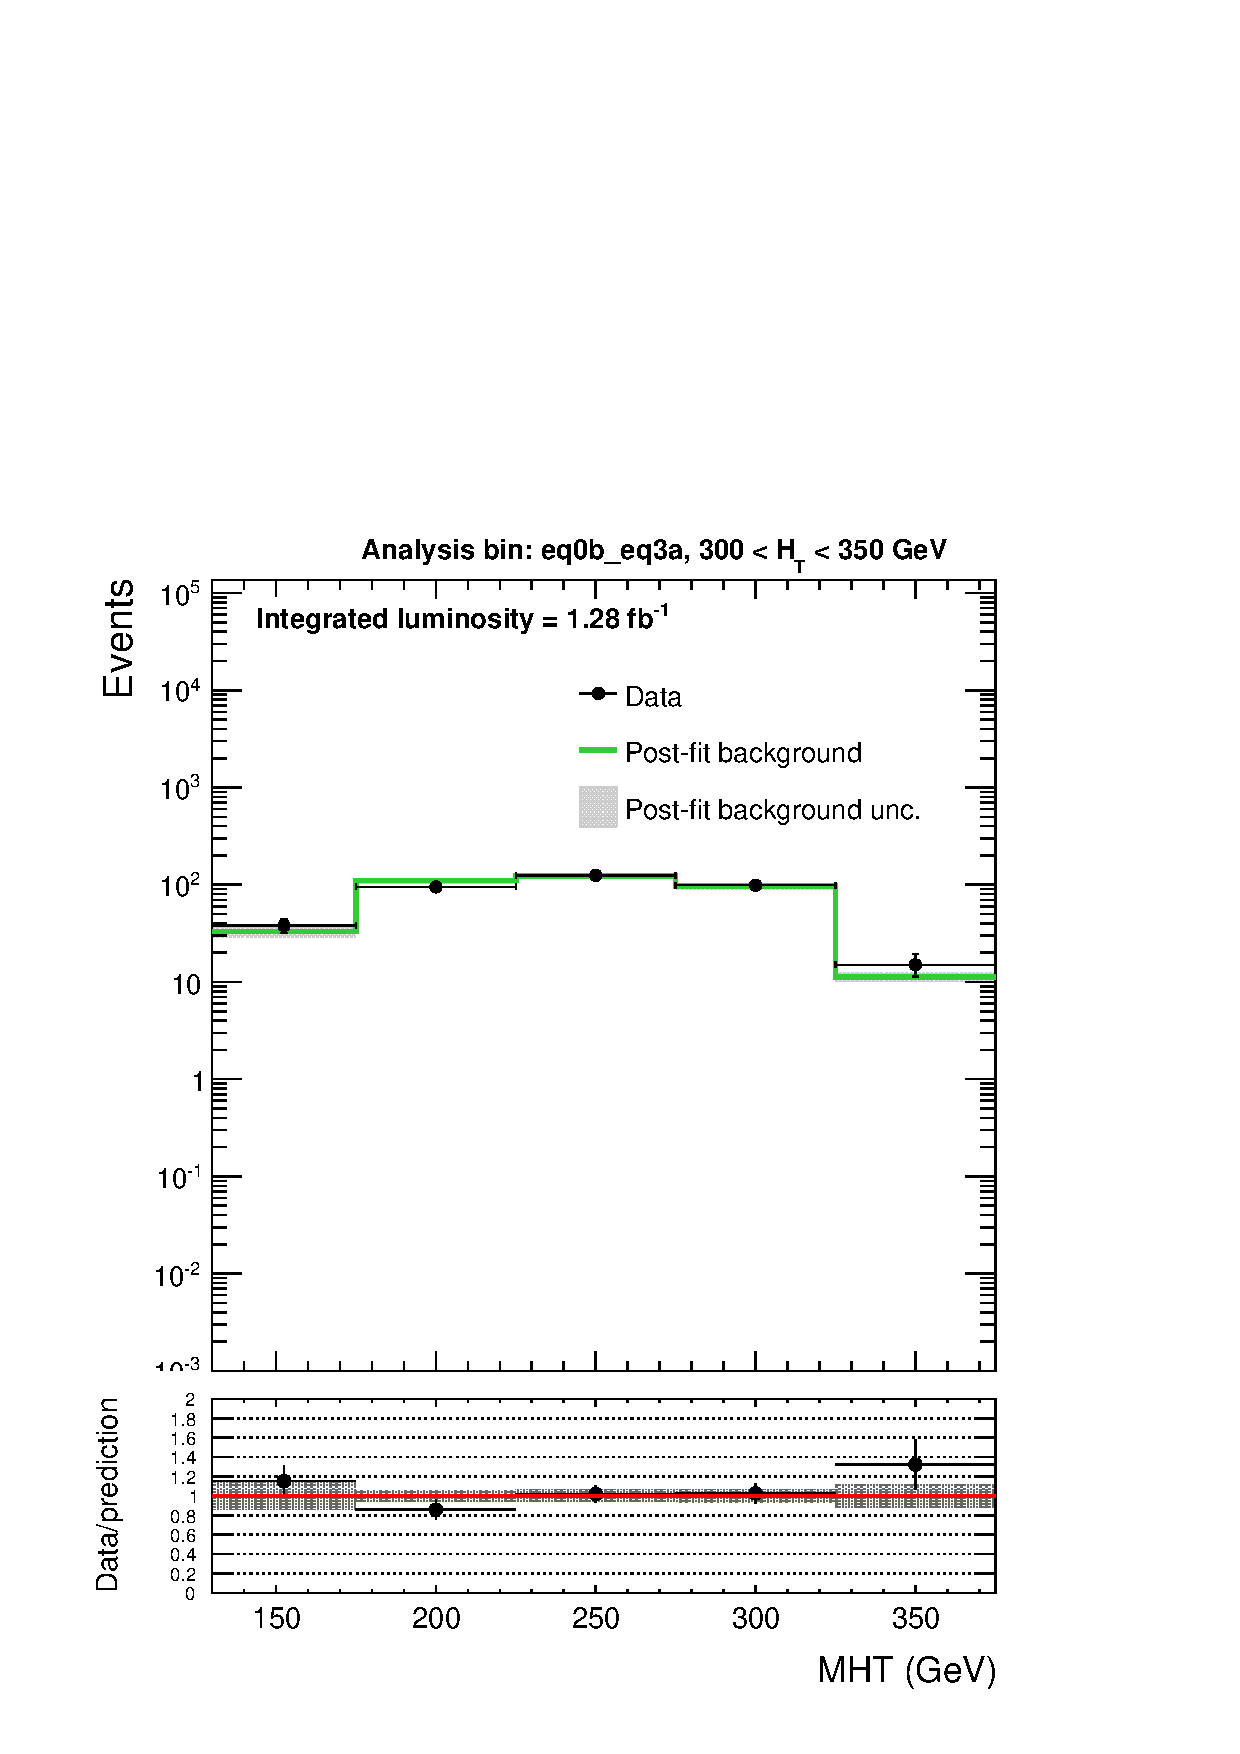
\includegraphics[width=0.25\textwidth]{figures/postFitResults/postFitShapes/postFitShape_eq0b_eq3a_300_350.pdf} }\\
    \subfigure[$\nj^{\mathrm{asym}}=3$, $\nb=0$, $350 < \scalht < 400 \; \mathrm{GeV}$]{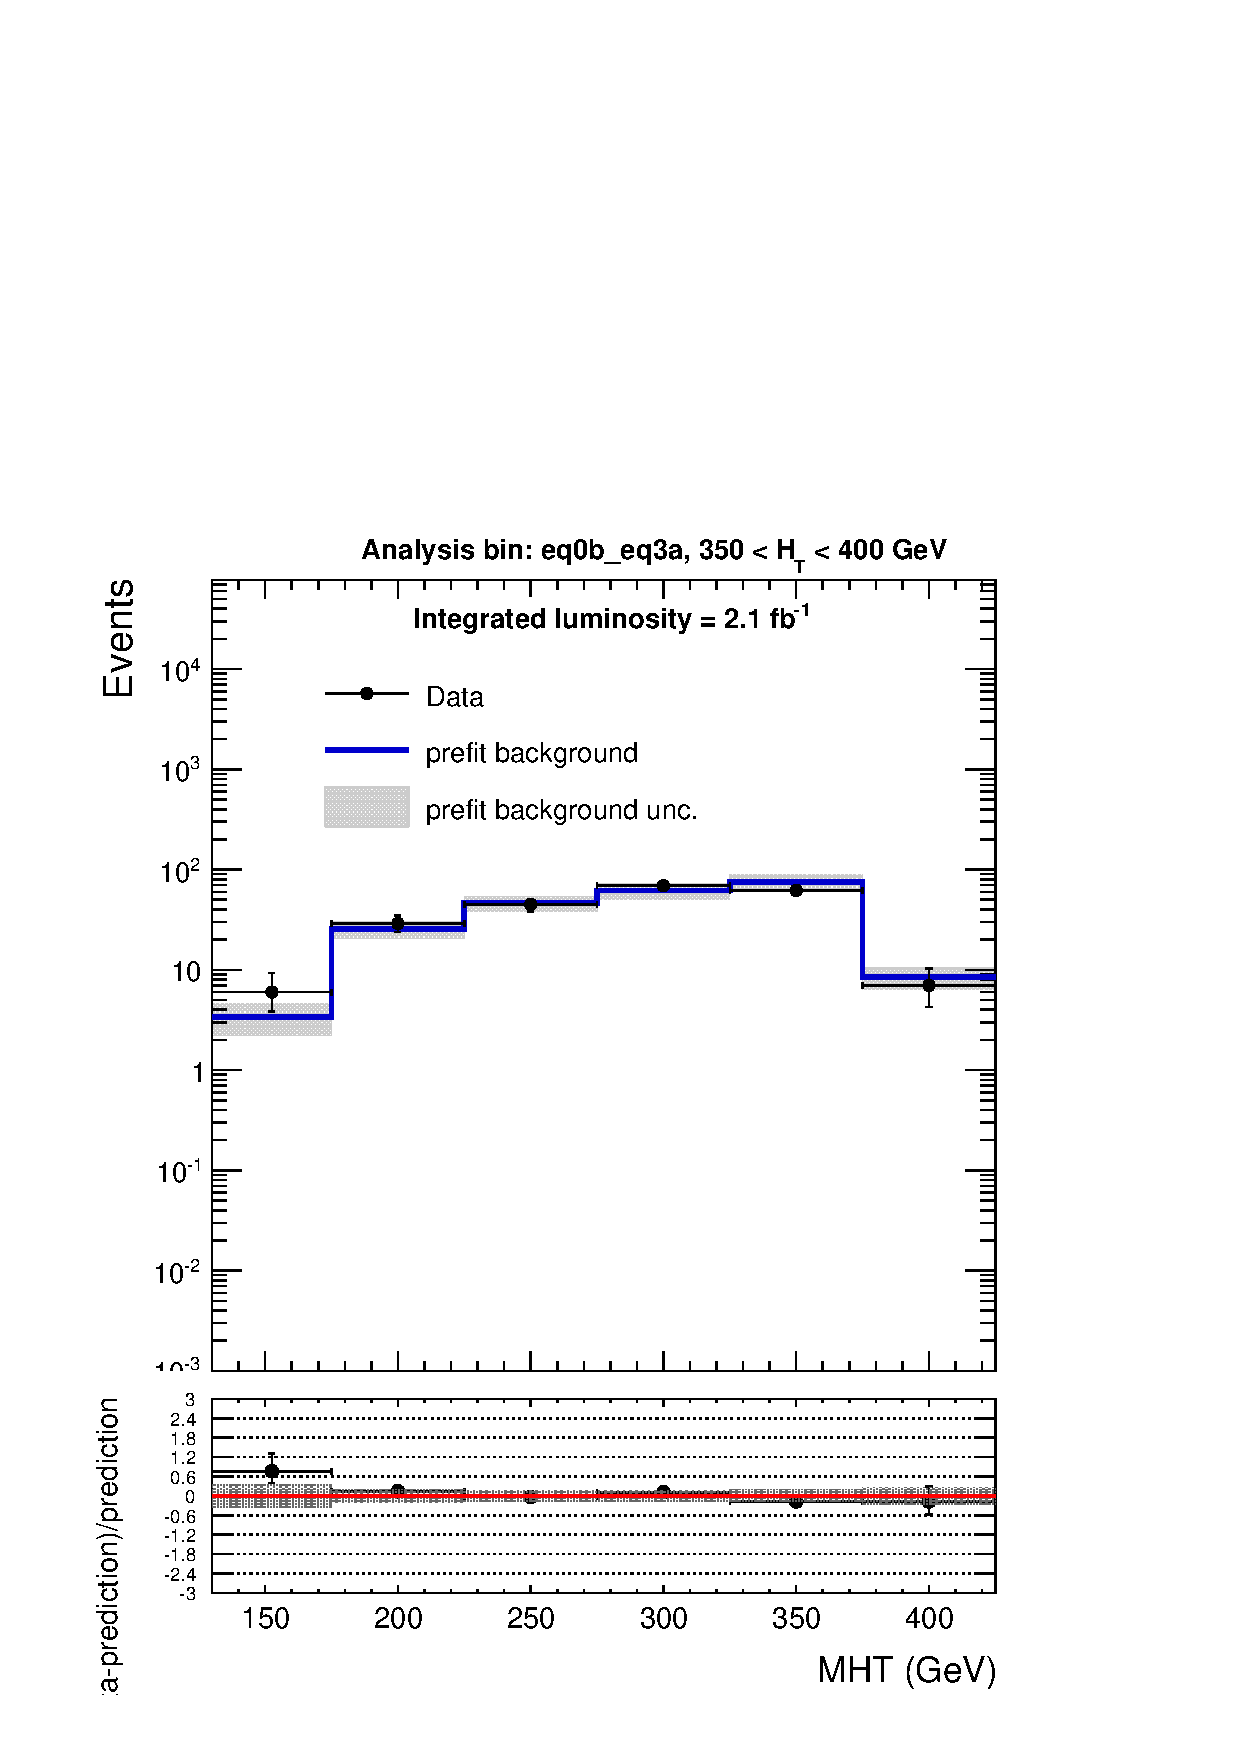
\includegraphics[width=0.25\textwidth]{figures/postFitResults/postFitShapes/postFitShape_eq0b_eq3a_350_400.pdf} }\hspace{1cm}
    \subfigure[$\nj^{\mathrm{asym}}=3$, $\nb=0$, $400 < \scalht < 500 \; \mathrm{GeV}$]{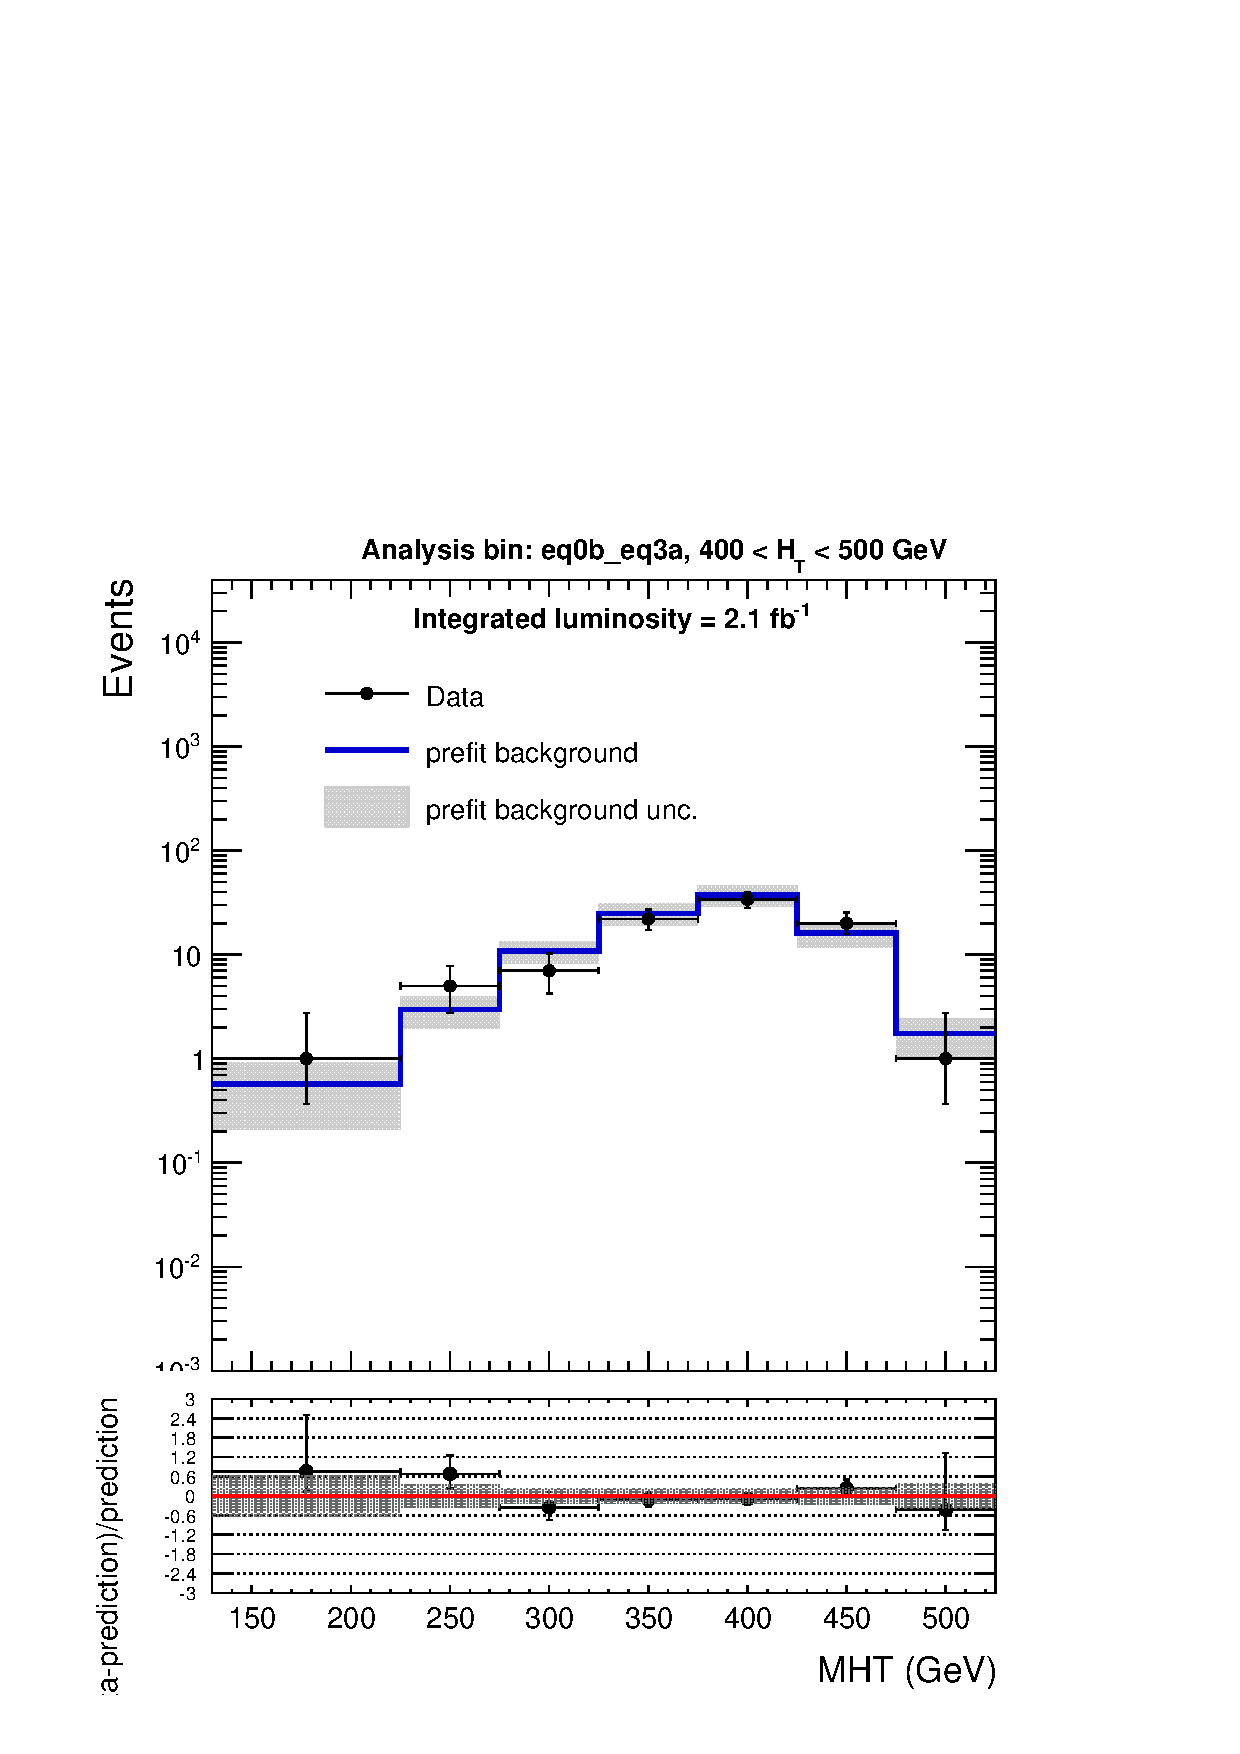
\includegraphics[width=0.25\textwidth]{figures/postFitResults/postFitShapes/postFitShape_eq0b_eq3a_400_500.pdf} }\hspace{1cm}
    \subfigure[$\nj^{\mathrm{asym}}=3$, $\nb=0$, $500 < \scalht < 600 \; \mathrm{GeV}$]{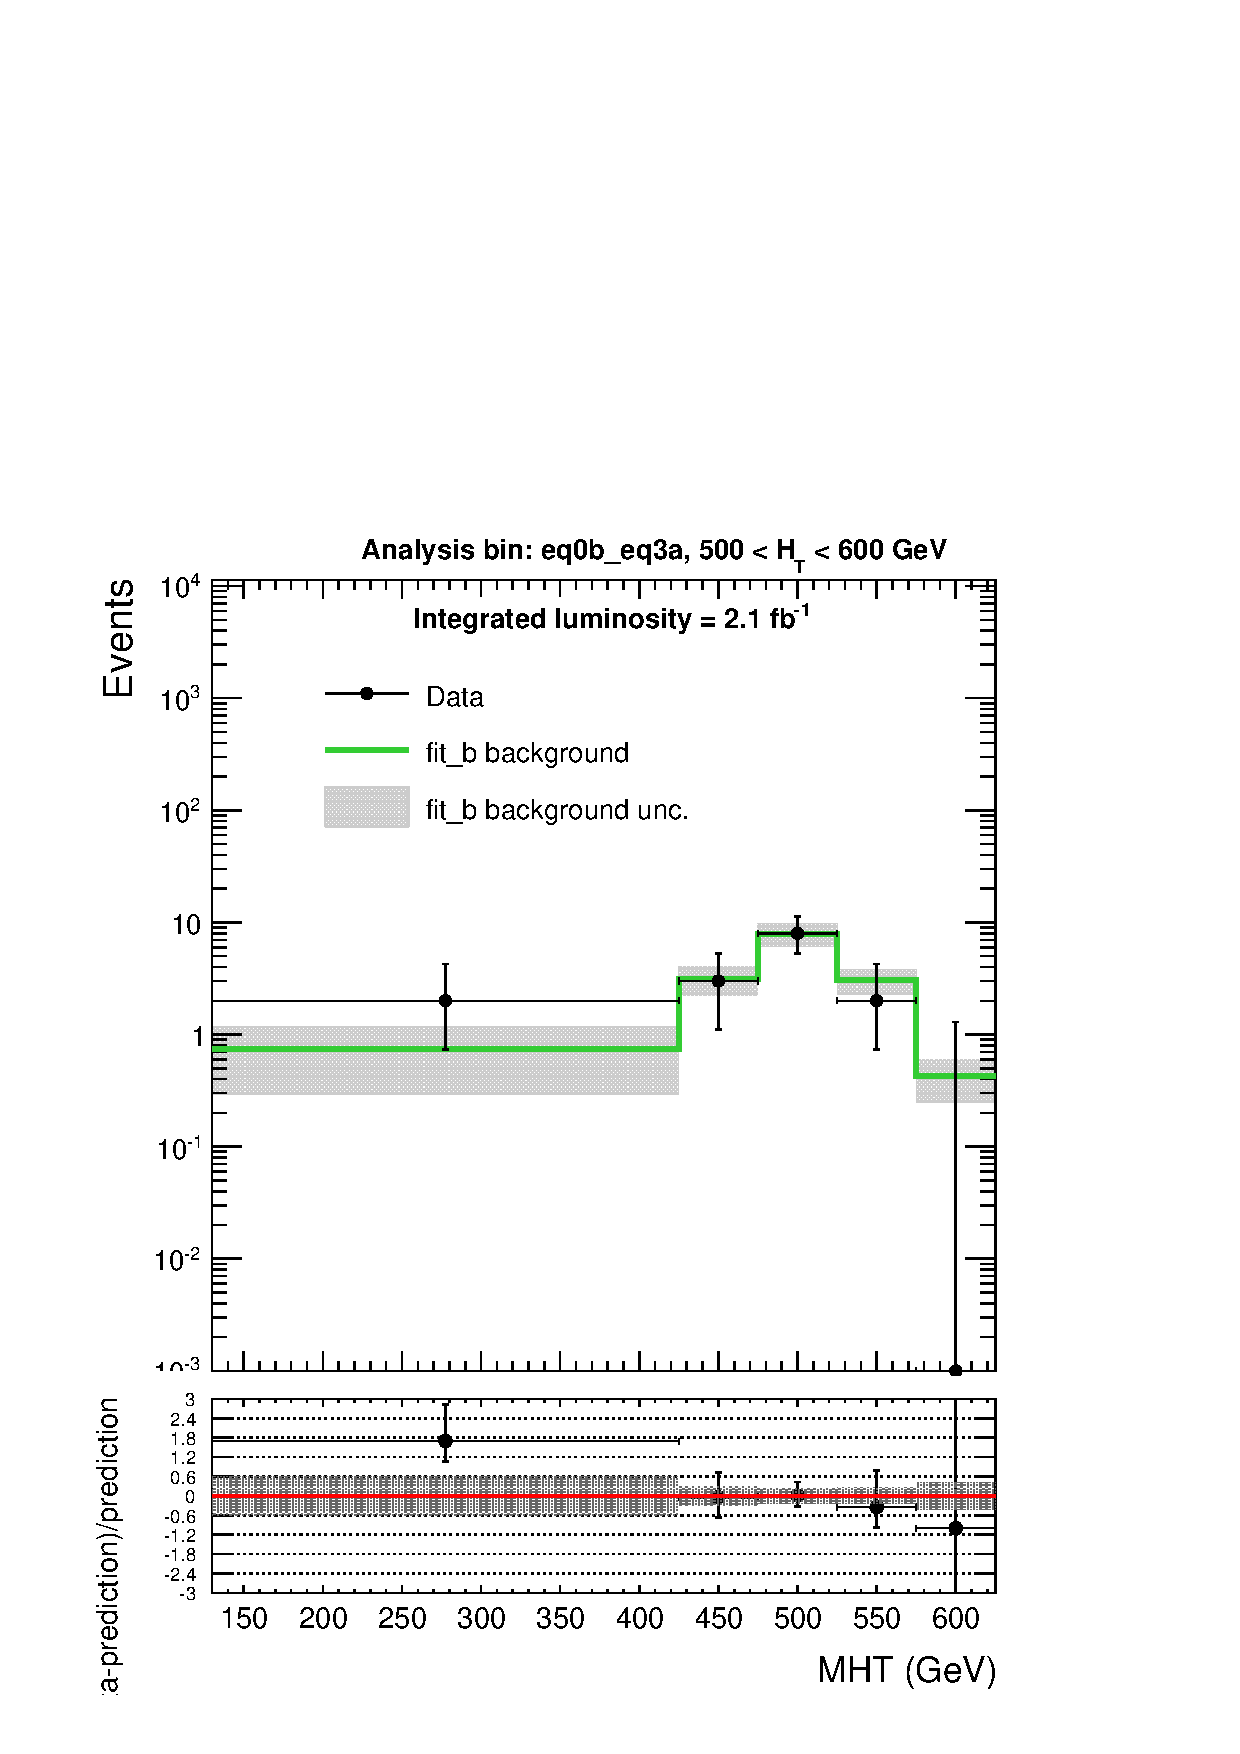
\includegraphics[width=0.25\textwidth]{figures/postFitResults/postFitShapes/postFitShape_eq0b_eq3a_500_600.pdf} }\\
    \subfigure[$\nj^{\mathrm{asym}}=3$, $\nb=0$, $\scalht > 600 \; \mathrm{GeV}$]{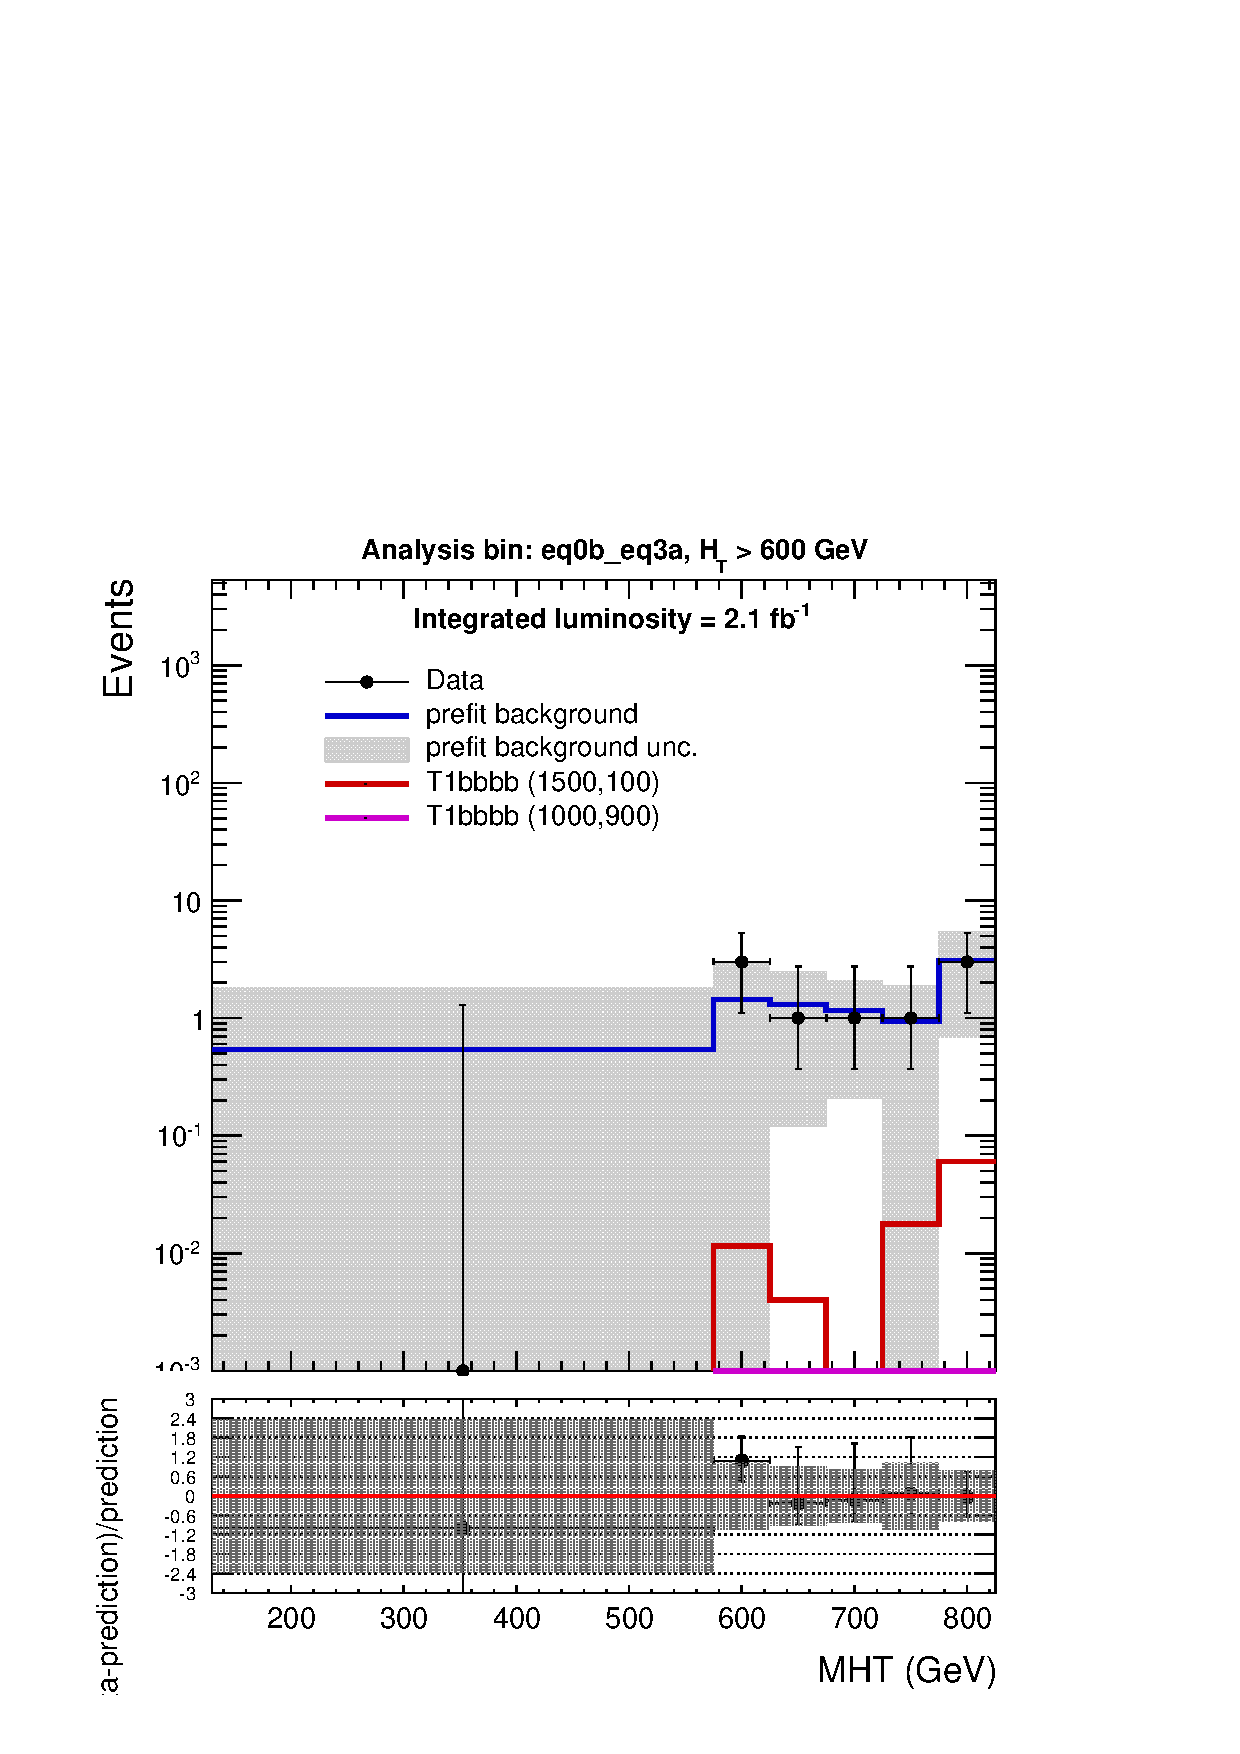
\includegraphics[width=0.25\textwidth]{figures/postFitResults/postFitShapes/postFitShape_eq0b_eq3a_600_Inf.pdf} }\hspace{1cm}
  \end{center}
\end{figure}



\newpage
\begin{figure}[h!]
\caption{Post-fit \MHT templates for the bin $\nj^{\mathrm{sym}}=3$, $\nb=0$ \label{fig:postFitShapes_eq0b_eq3j}}.
\begin{center}

    \subfigure[$\nj^{\mathrm{sym}}=3$, $\nb=0$, $250 < \scalht < 300 \; \mathrm{GeV}$]{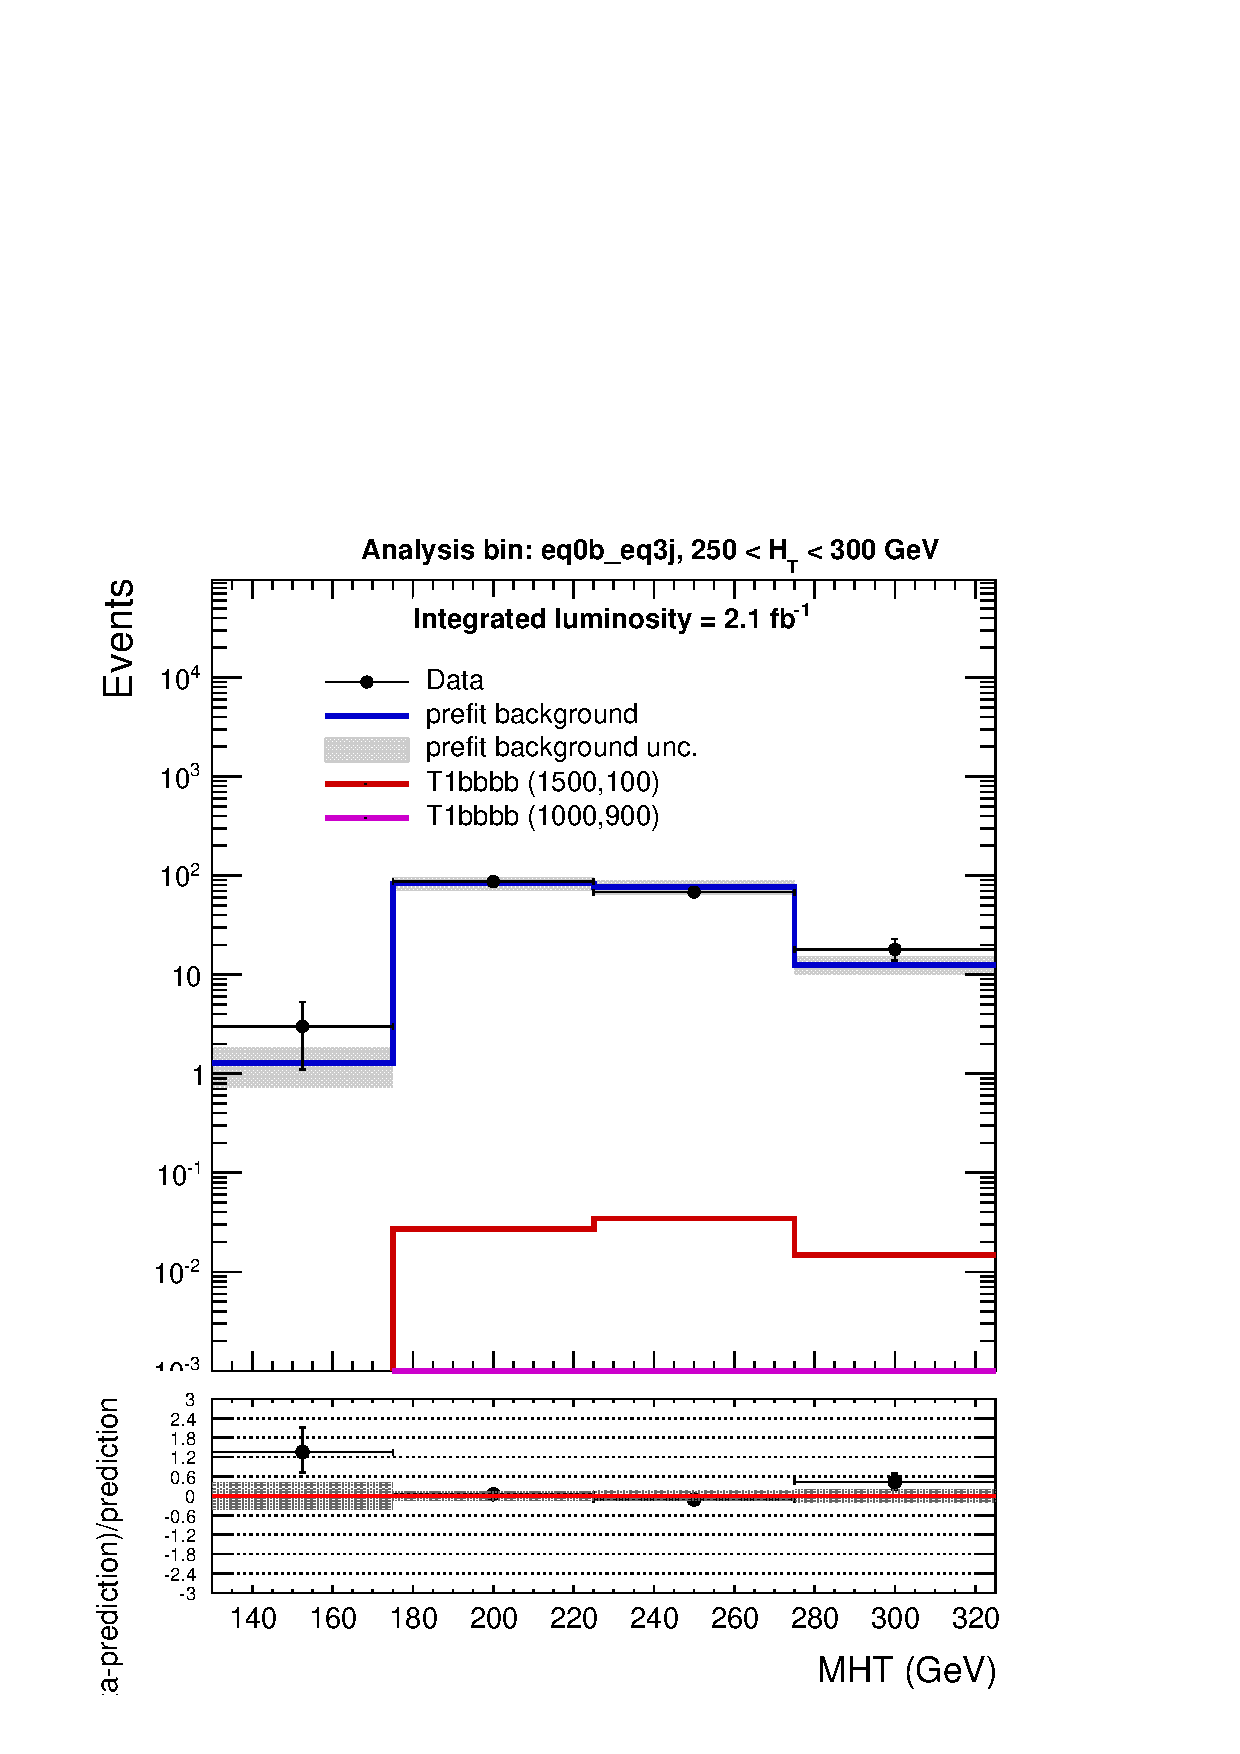
\includegraphics[width=0.25\textwidth]{figures/postFitResults/postFitShapes/postFitShape_eq0b_eq3j_250_300.pdf} }\hspace{1cm}
    \subfigure[$\nj^{\mathrm{sym}}=3$, $\nb=0$, $300 < \scalht < 350 \; \mathrm{GeV}$]{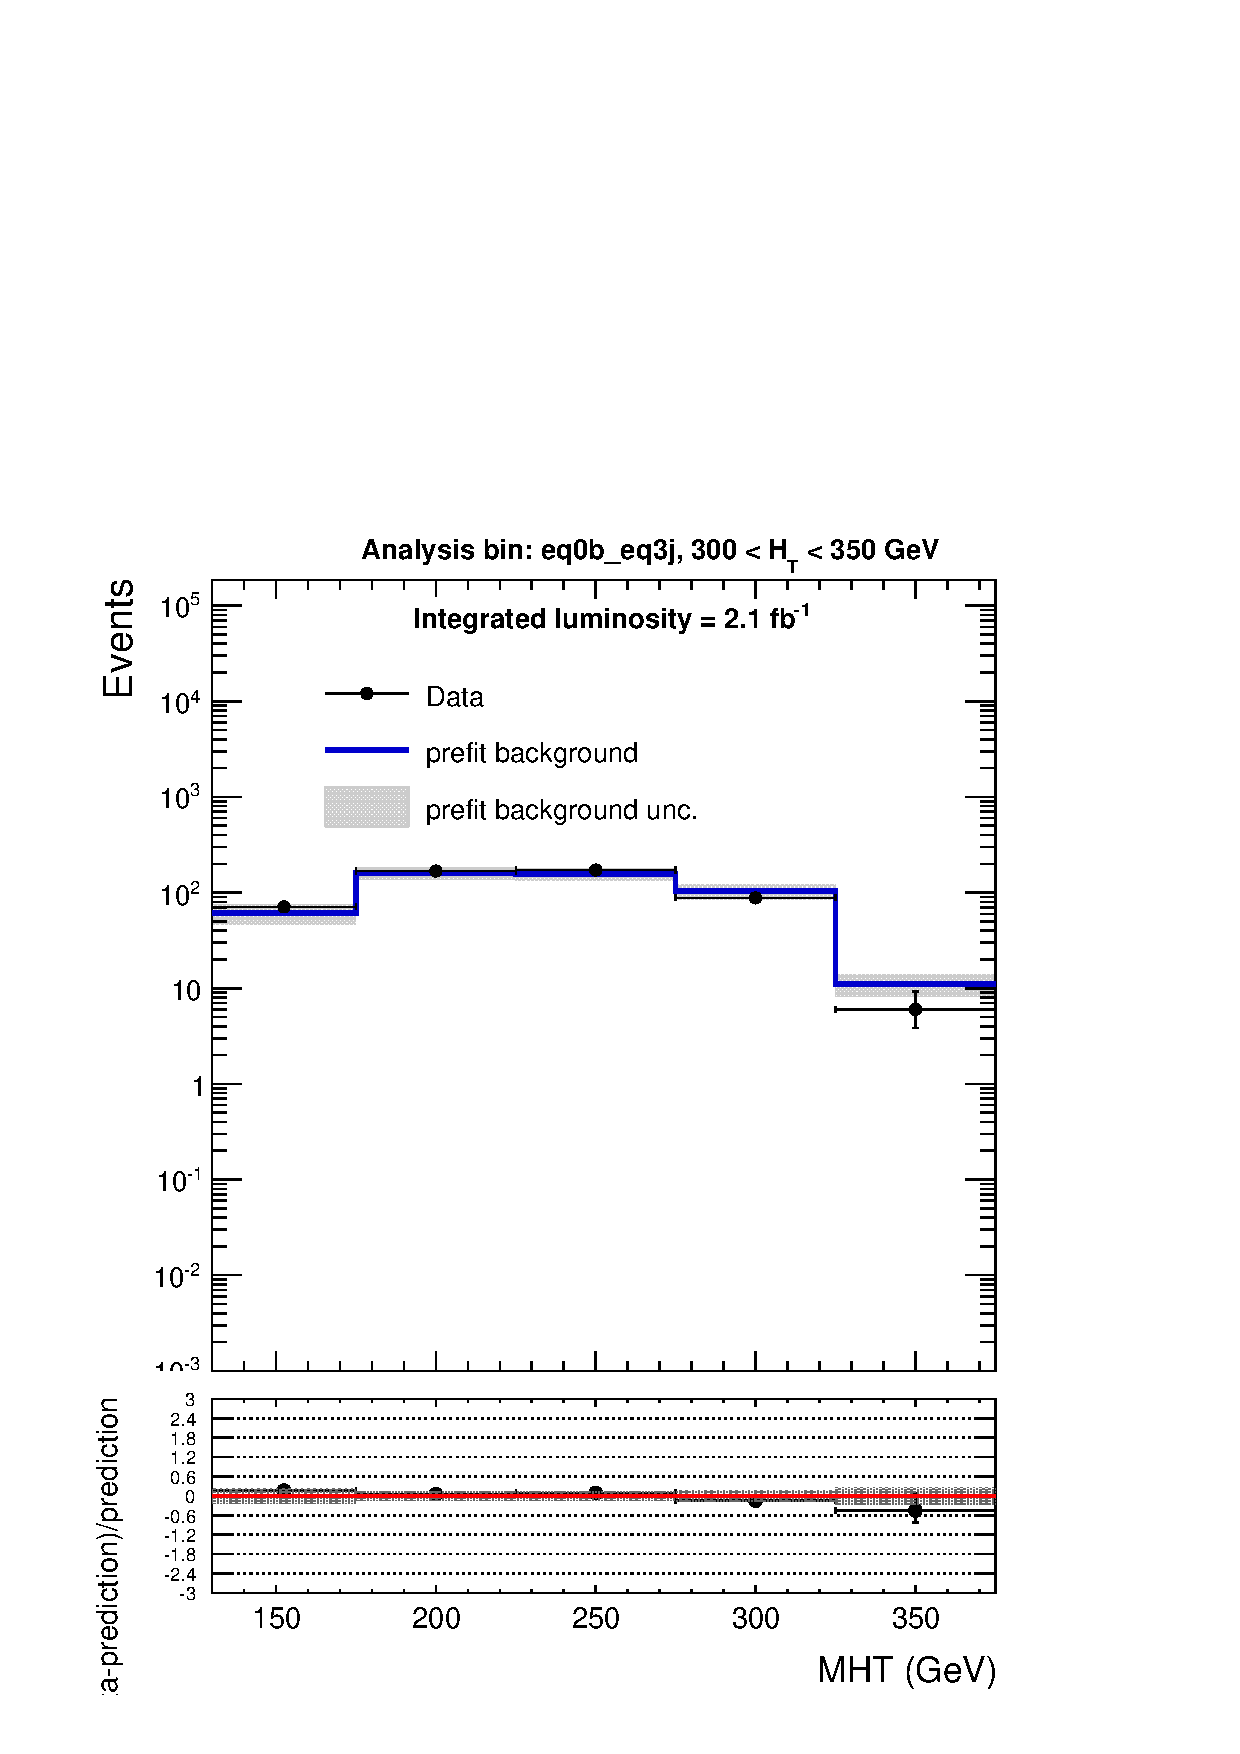
\includegraphics[width=0.25\textwidth]{figures/postFitResults/postFitShapes/postFitShape_eq0b_eq3j_300_350.pdf} }\hspace{1cm}
    \subfigure[$\nj^{\mathrm{sym}}=3$, $\nb=0$, $350 < \scalht < 400 \; \mathrm{GeV}$]{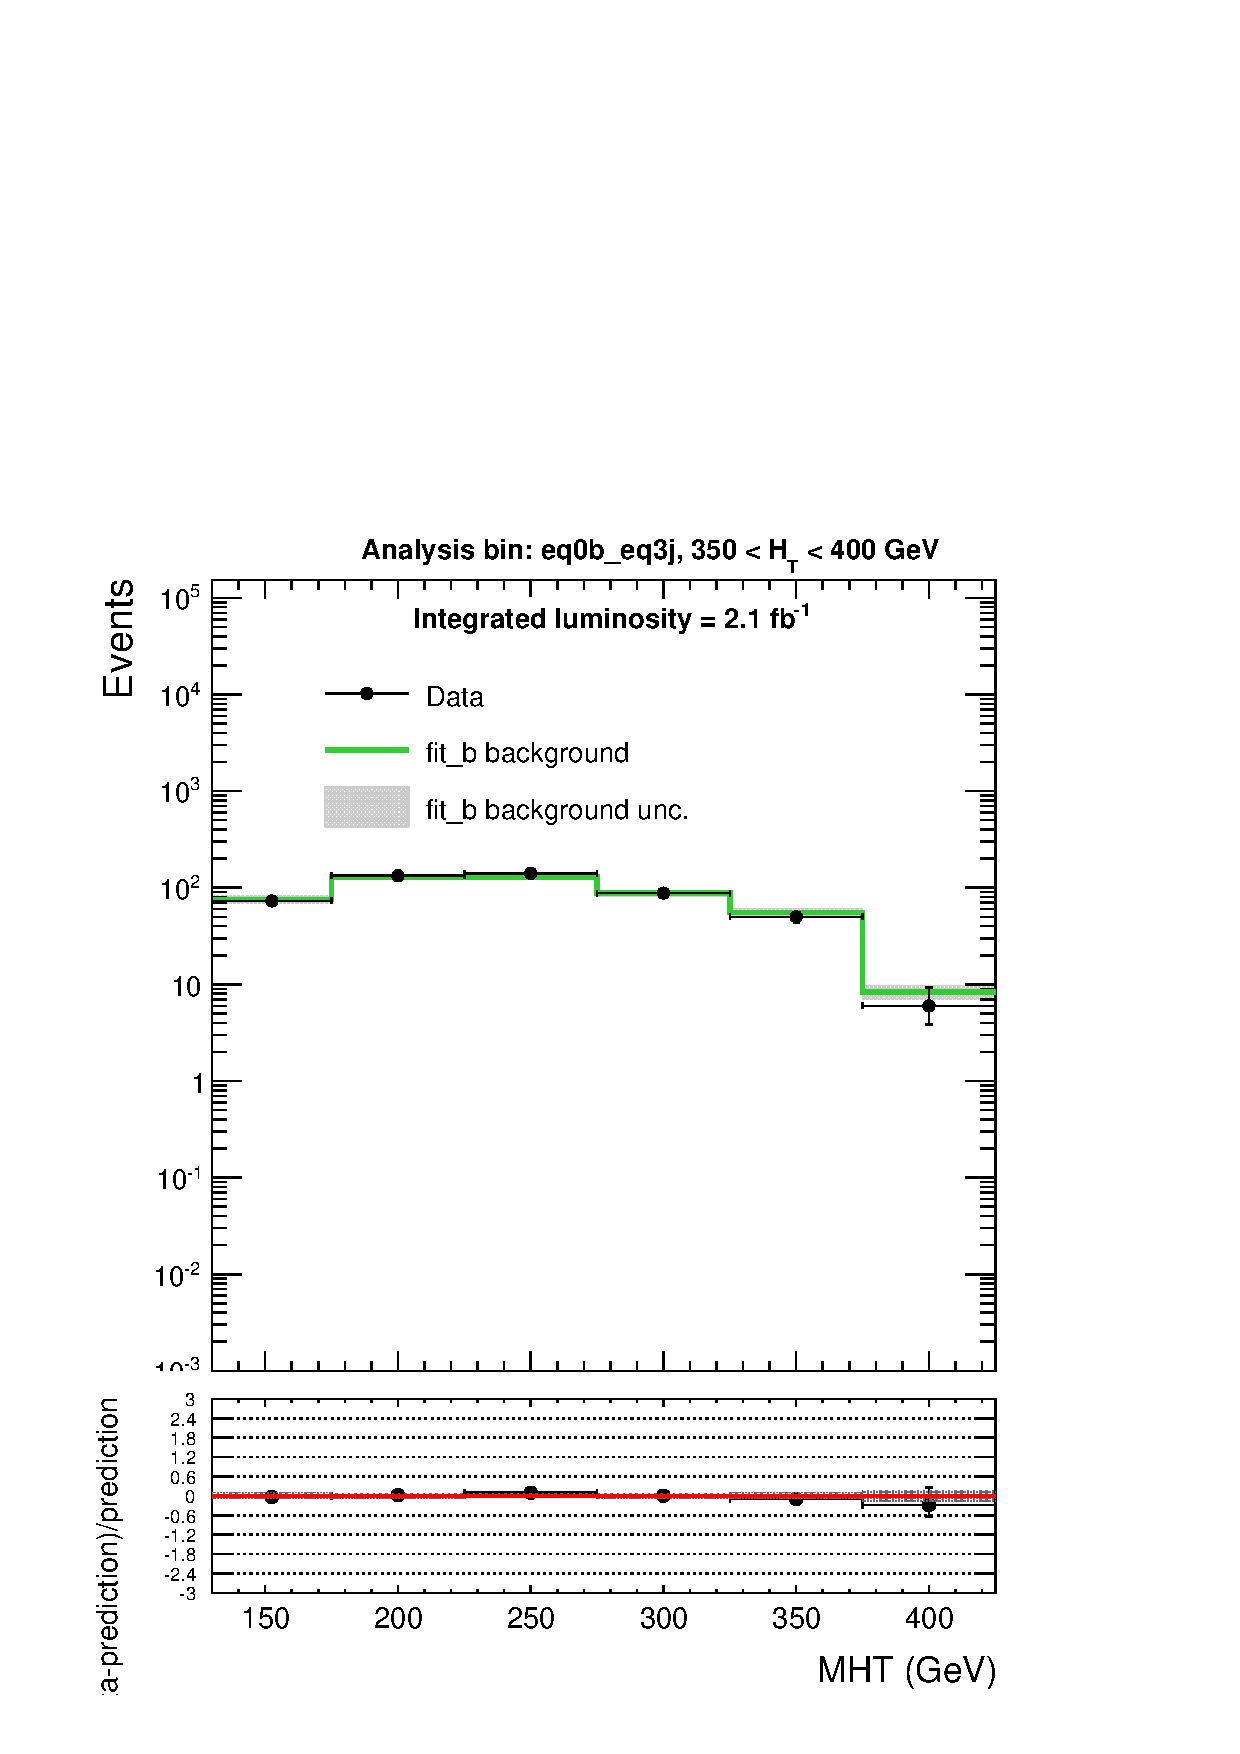
\includegraphics[width=0.25\textwidth]{figures/postFitResults/postFitShapes/postFitShape_eq0b_eq3j_350_400.pdf} }\\
    \subfigure[$\nj^{\mathrm{sym}}=3$, $\nb=0$, $400 < \scalht < 500 \; \mathrm{GeV}$]{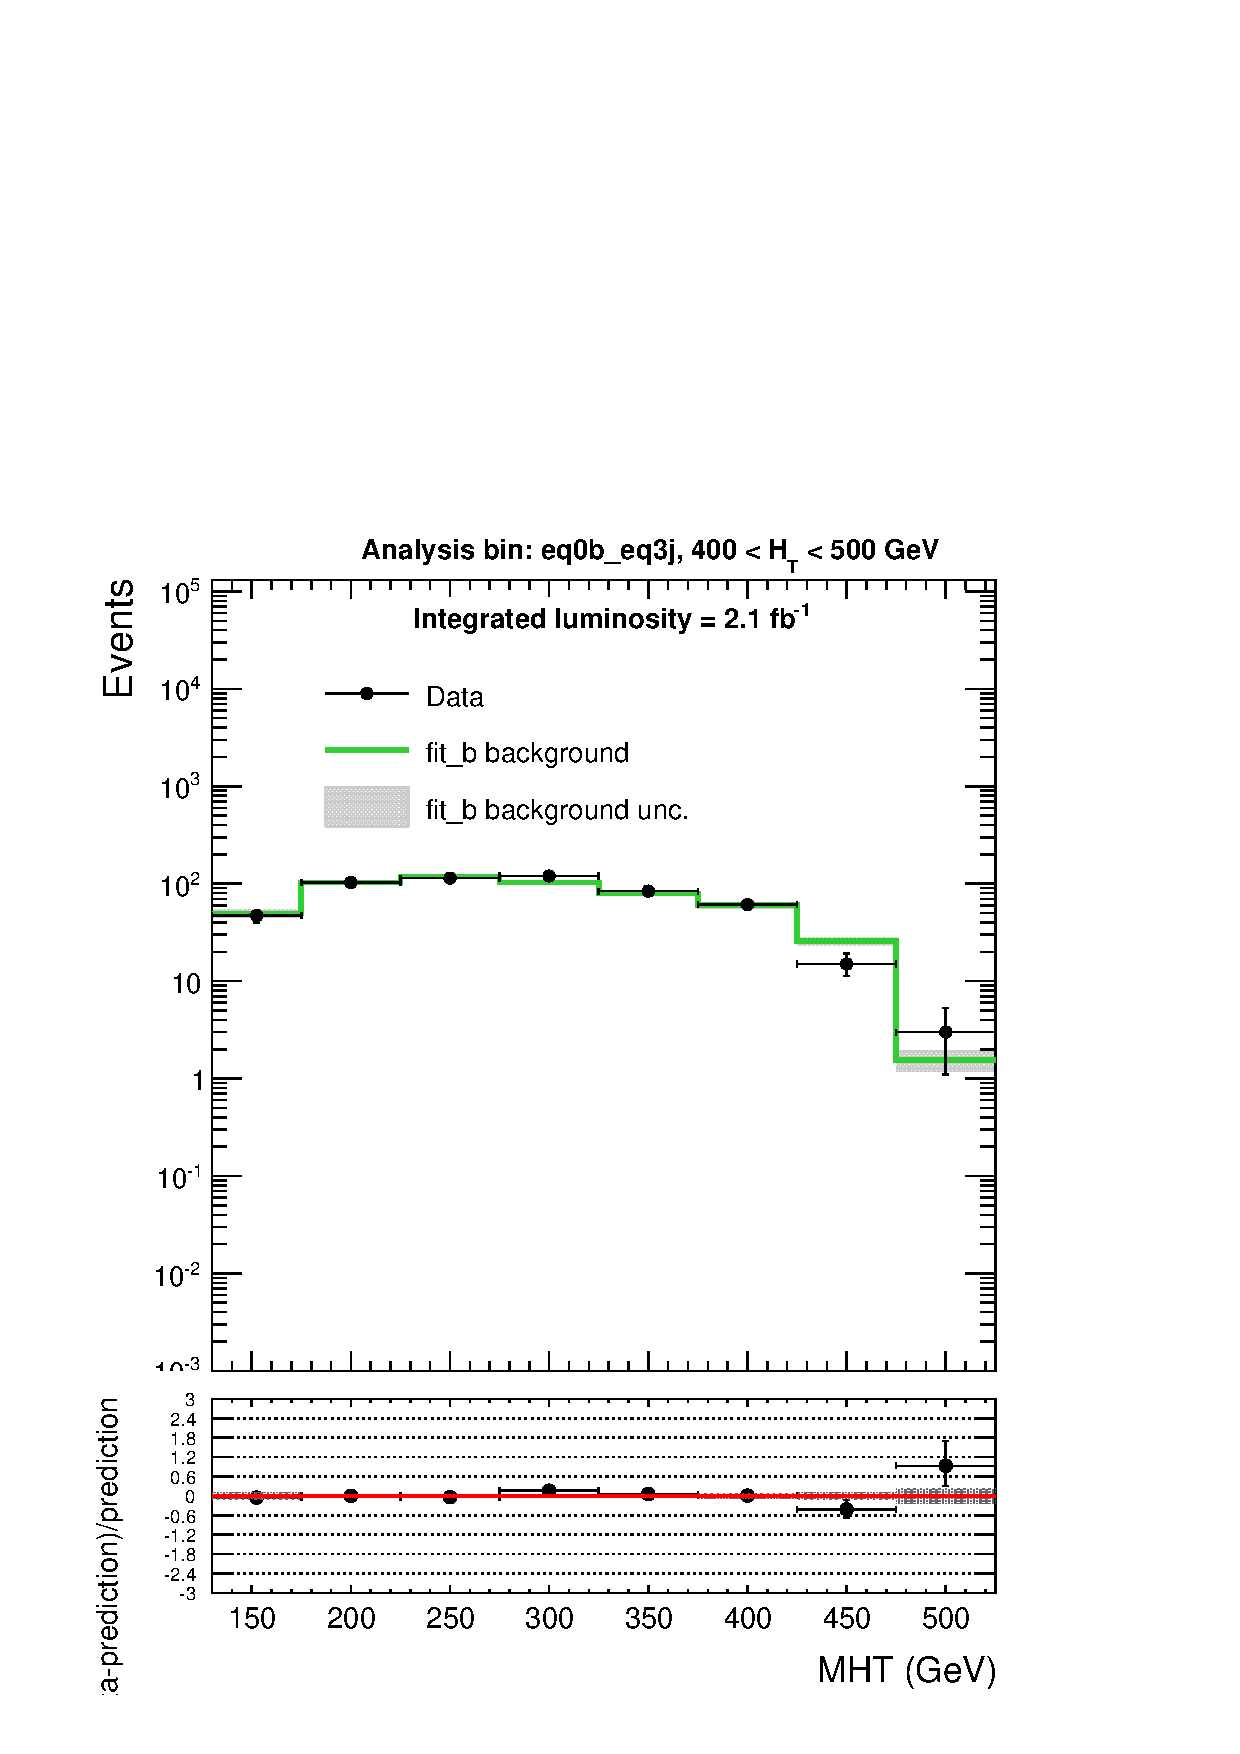
\includegraphics[width=0.25\textwidth]{figures/postFitResults/postFitShapes/postFitShape_eq0b_eq3j_400_500.pdf} }\hspace{1cm}
    \subfigure[$\nj^{\mathrm{sym}}=3$, $\nb=0$, $500 < \scalht < 600 \; \mathrm{GeV}$]{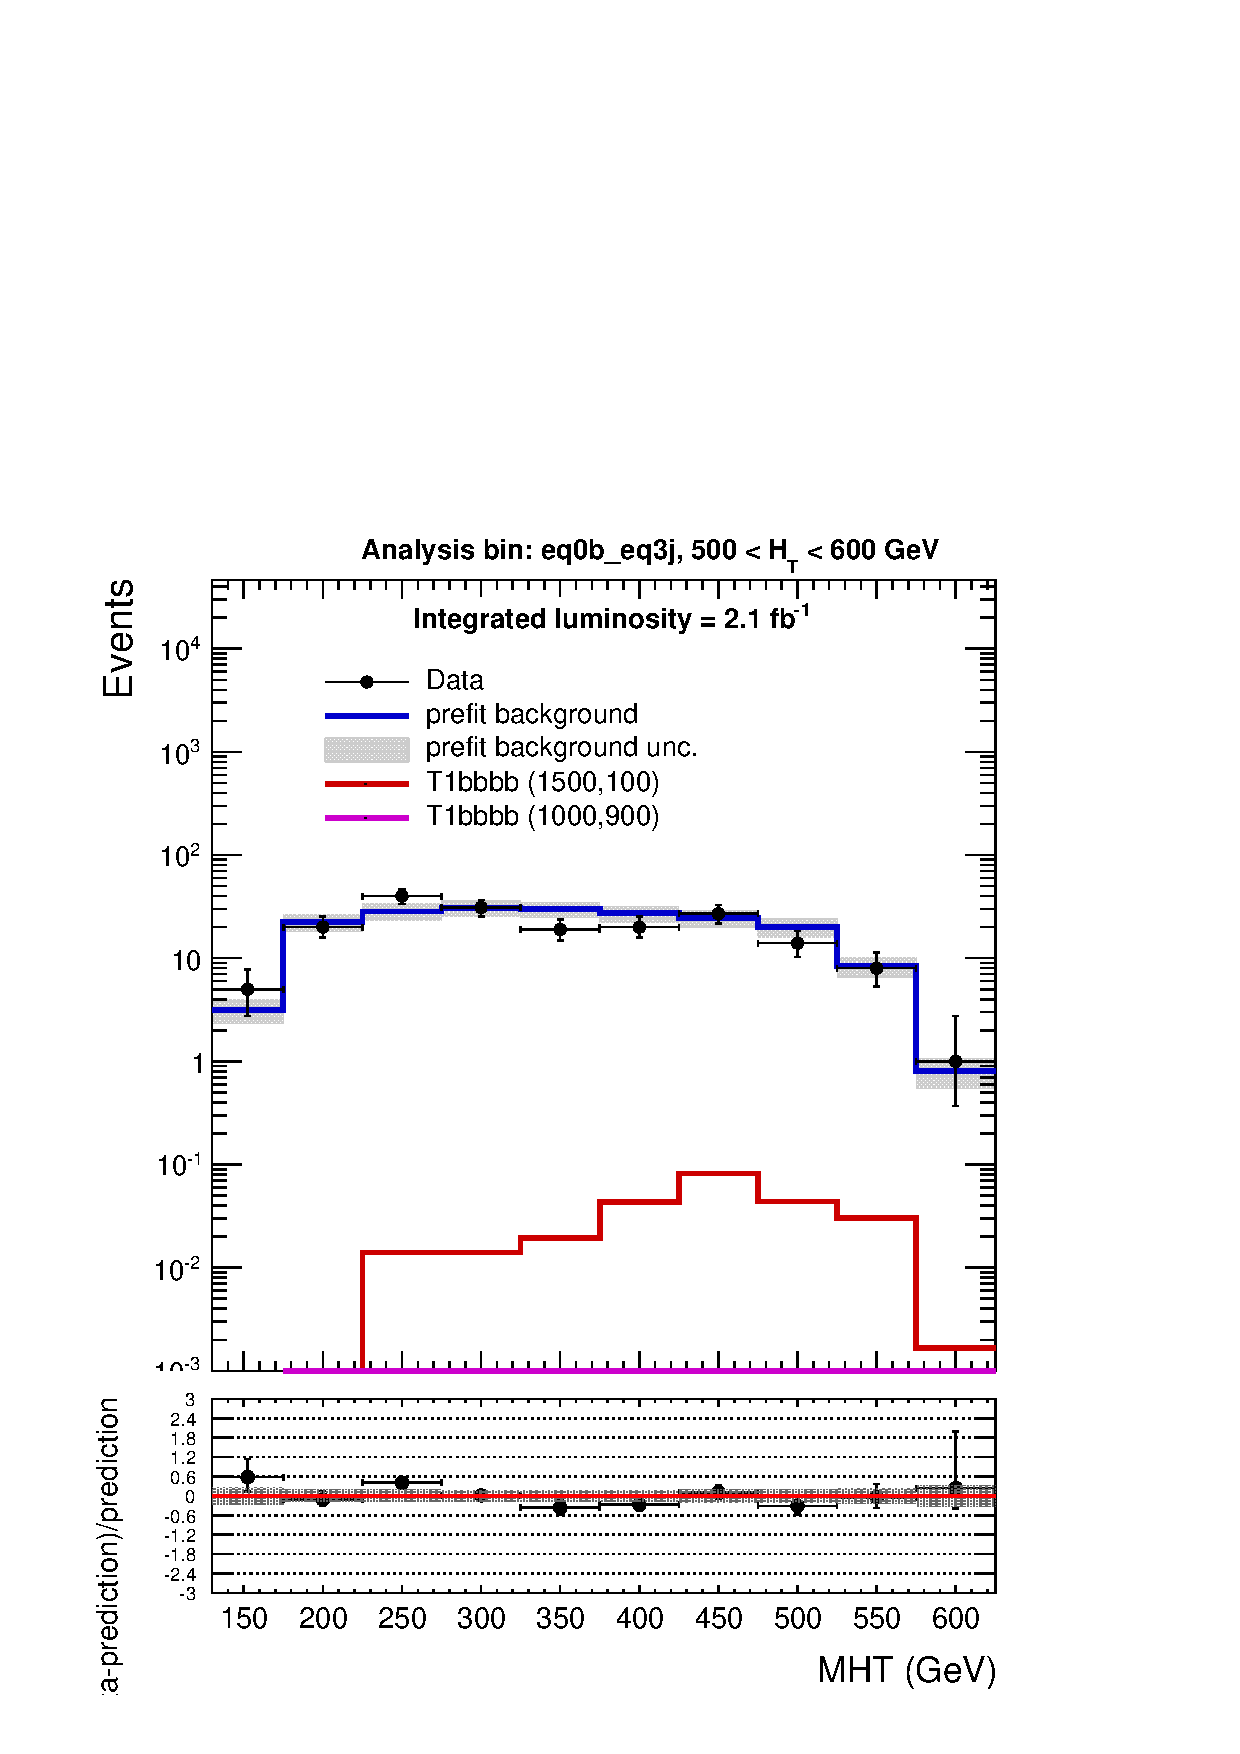
\includegraphics[width=0.25\textwidth]{figures/postFitResults/postFitShapes/postFitShape_eq0b_eq3j_500_600.pdf} }\hspace{1cm}
    \subfigure[$\nj^{\mathrm{sym}}=3$, $\nb=0$, $600 < \scalht < 800 \; \mathrm{GeV}$]{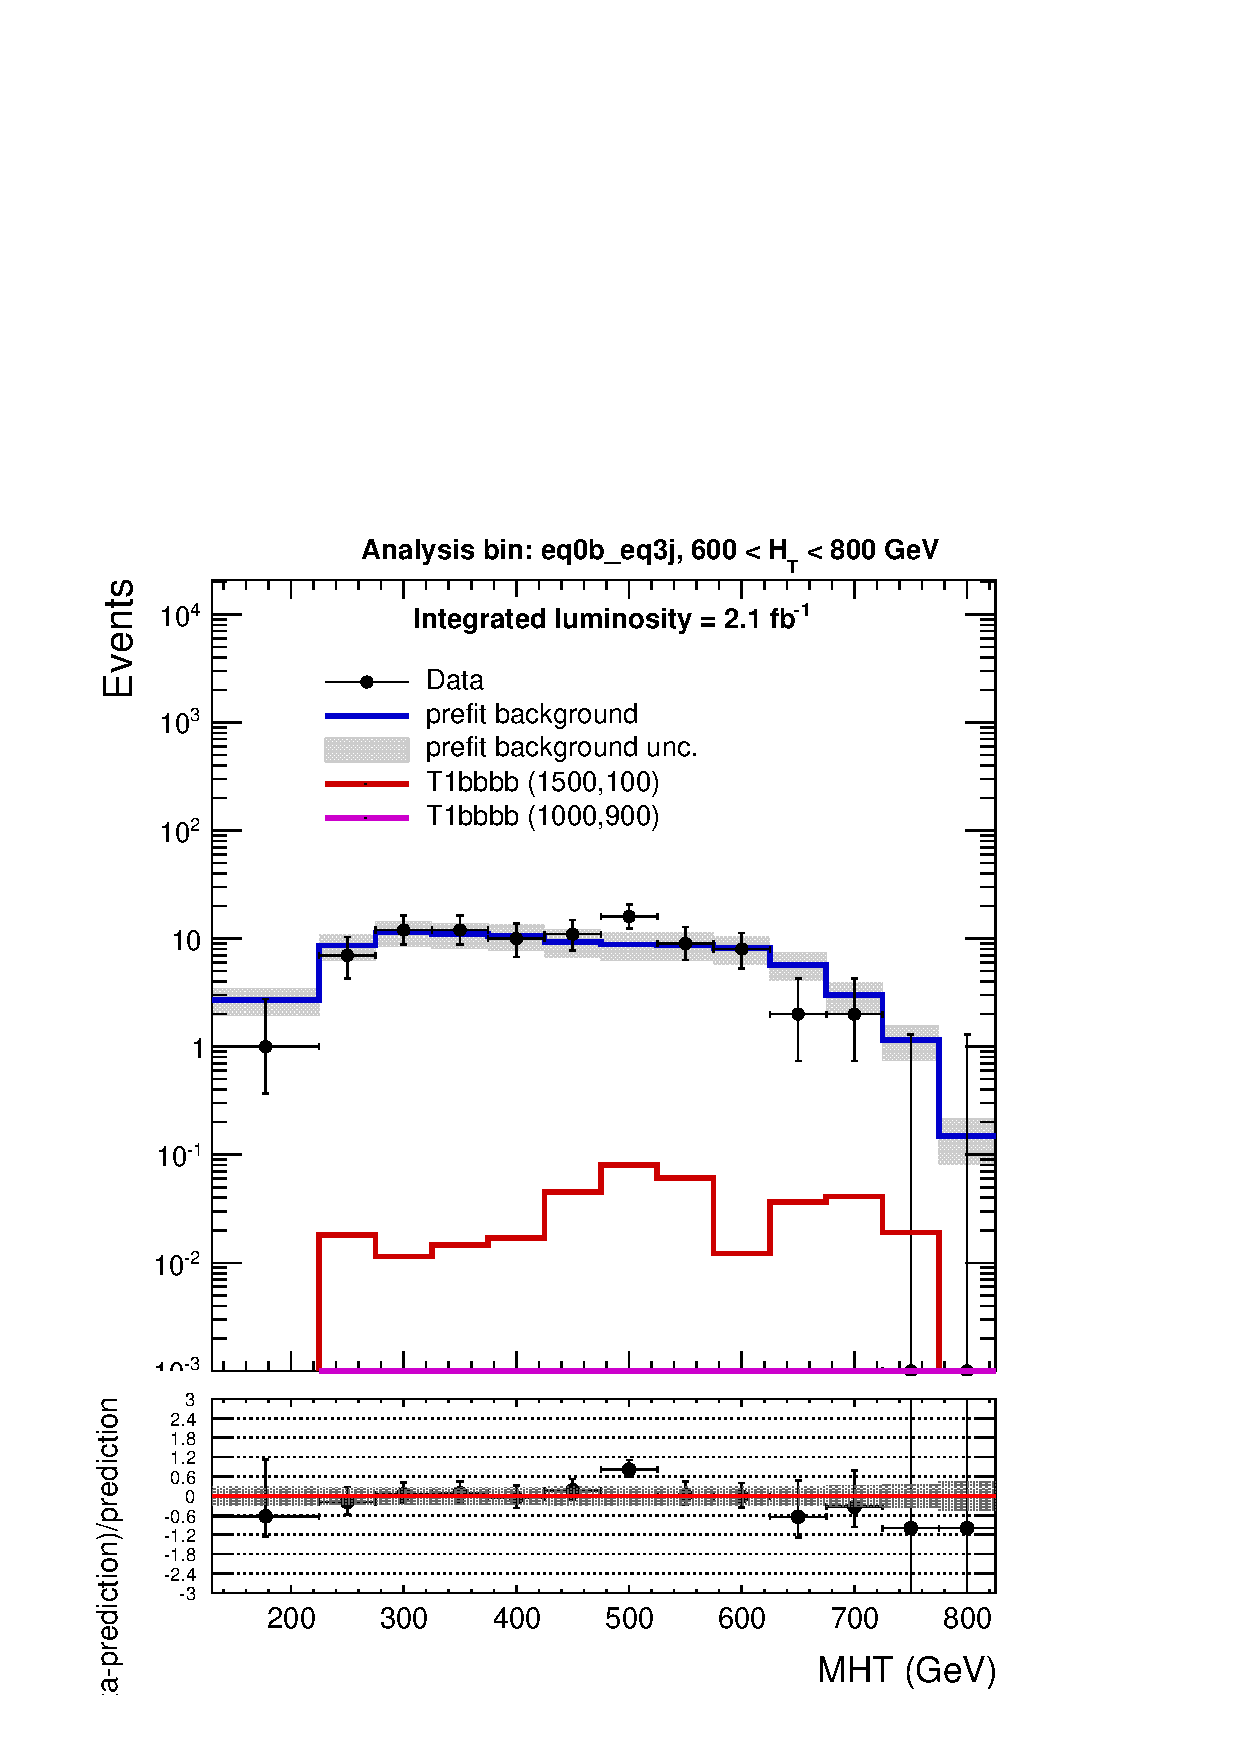
\includegraphics[width=0.25\textwidth]{figures/postFitResults/postFitShapes/postFitShape_eq0b_eq3j_600_800.pdf} }\\
    \subfigure[$\nj^{\mathrm{sym}}=3$, $\nb=0$, $\scalht > 800 \; \mathrm{GeV}$]{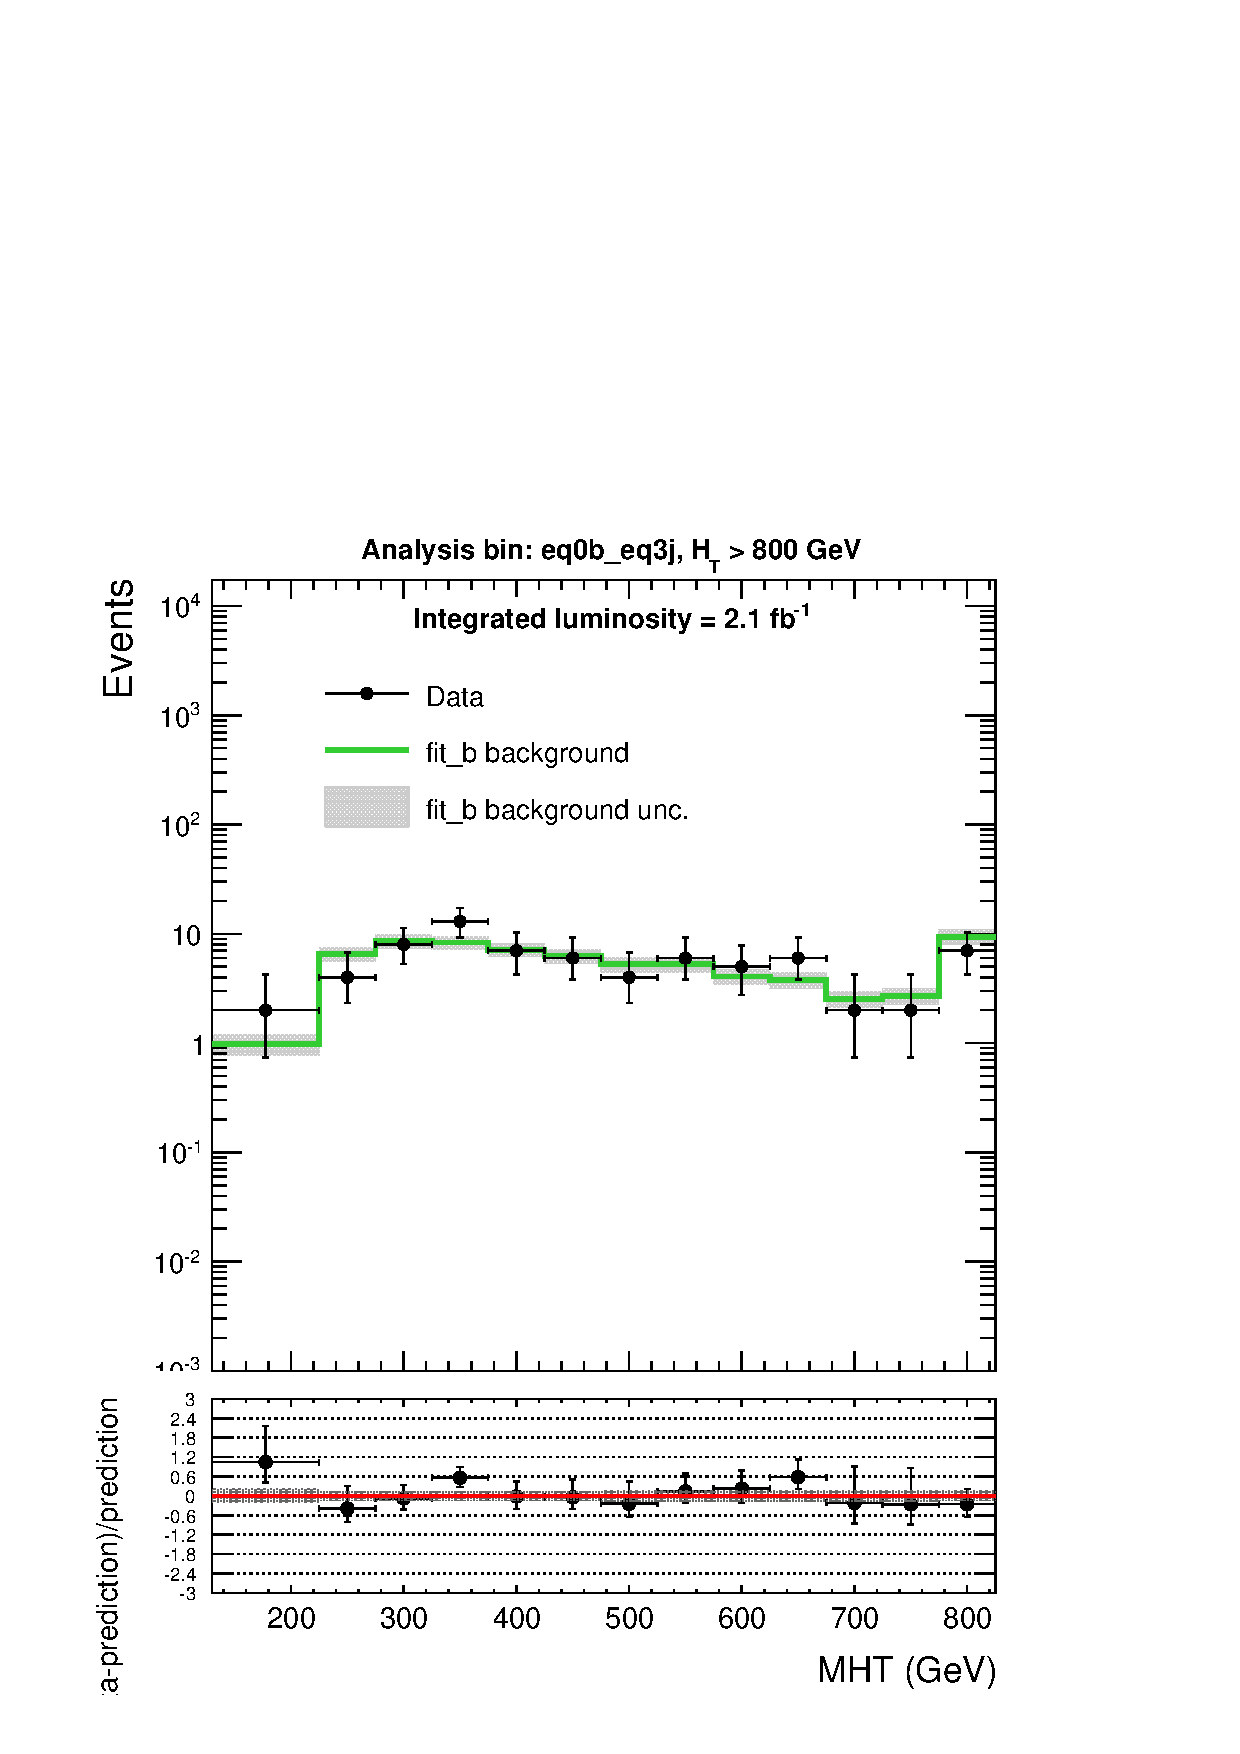
\includegraphics[width=0.25\textwidth]{figures/postFitResults/postFitShapes/postFitShape_eq0b_eq3j_800_Inf.pdf} }\hspace{1cm}
  \end{center}
\end{figure}



\newpage
\begin{figure}[h!]
\caption{Post-fit \MHT templates for the bin $\nj^{\mathrm{asym}}=4$, $\nb=0$ \label{fig:postFitShapes_eq0b_eq4a}}.
\begin{center}

    \subfigure[$\nj^{\mathrm{asym}}=4$, $\nb=0$, $200 < \scalht < 250 \; \mathrm{GeV}$]{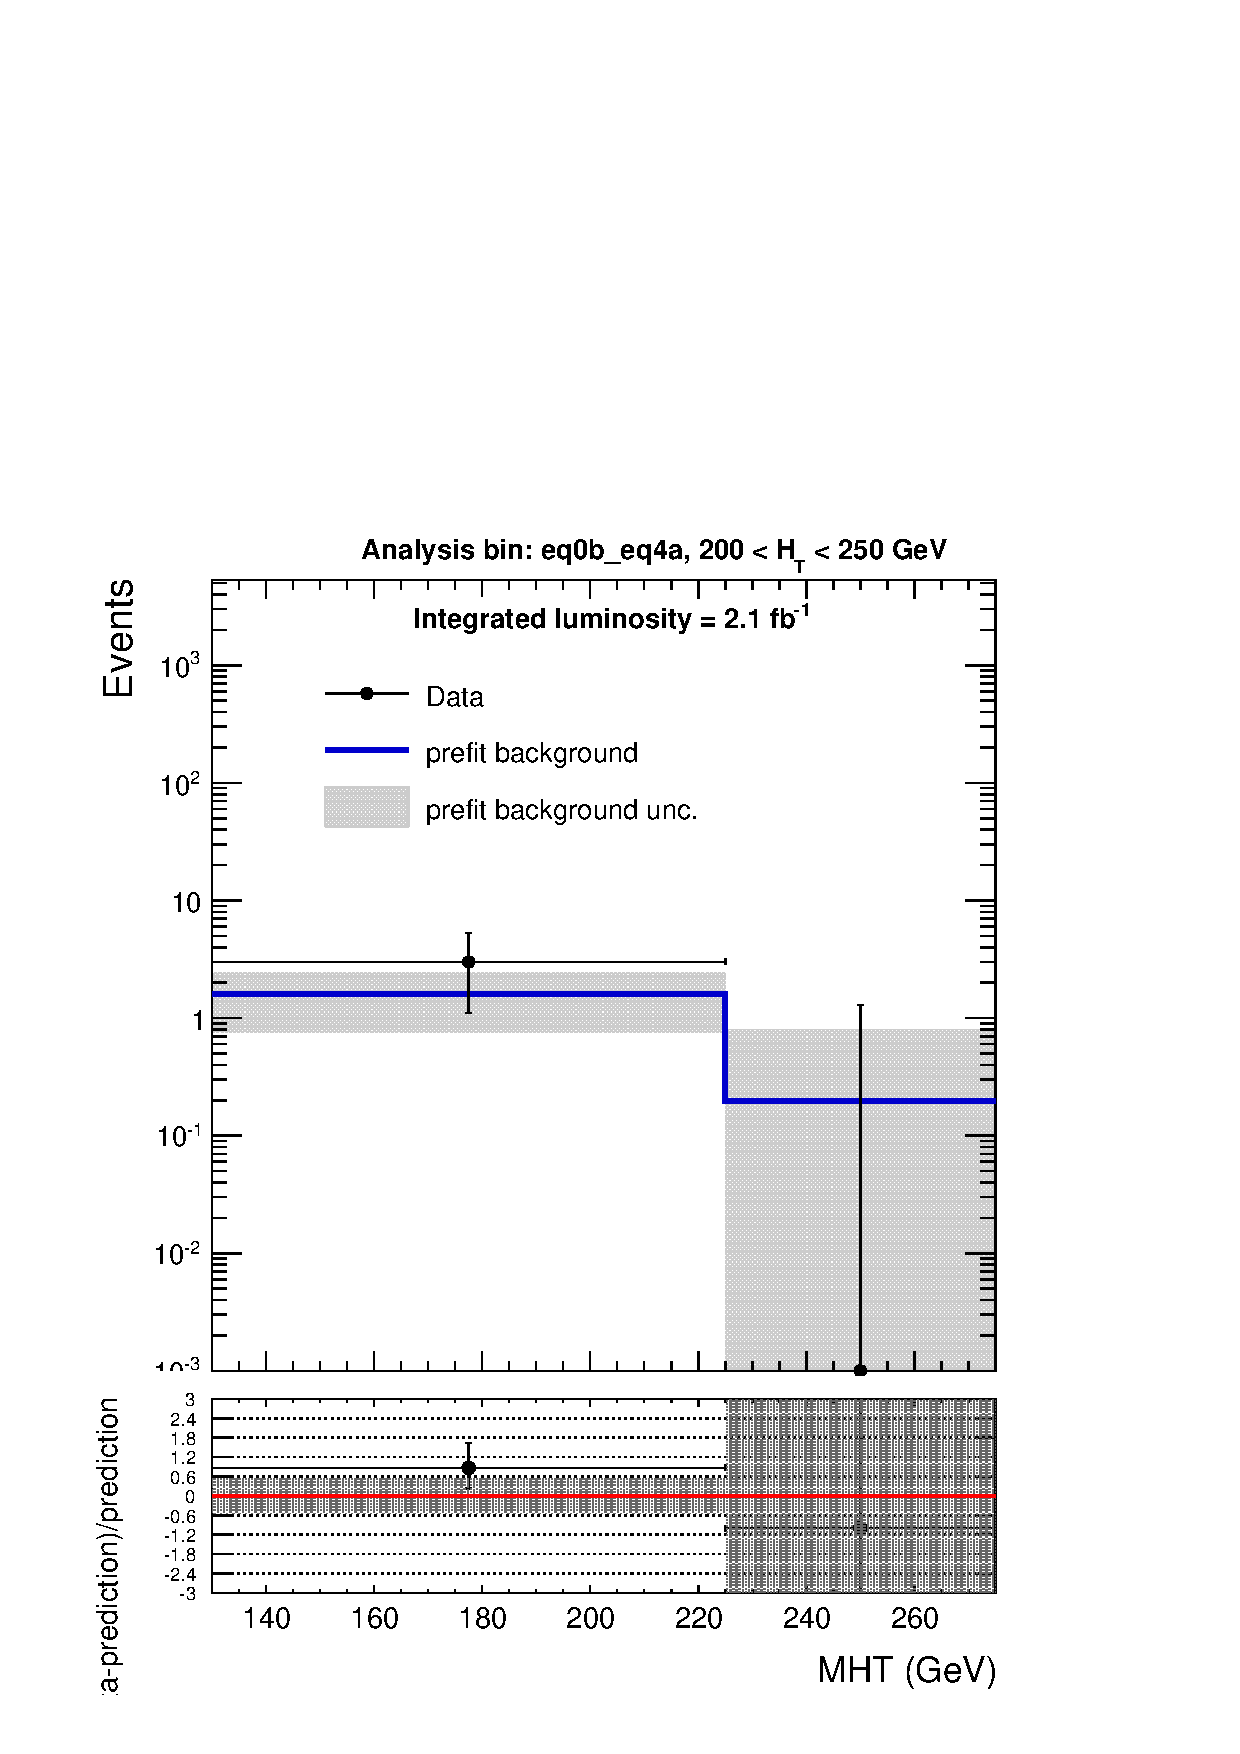
\includegraphics[width=0.25\textwidth]{figures/postFitResults/postFitShapes/postFitShape_eq0b_eq4a_200_250.pdf} }\hspace{1cm}
    \subfigure[$\nj^{\mathrm{asym}}=4$, $\nb=0$, $250 < \scalht < 300 \; \mathrm{GeV}$]{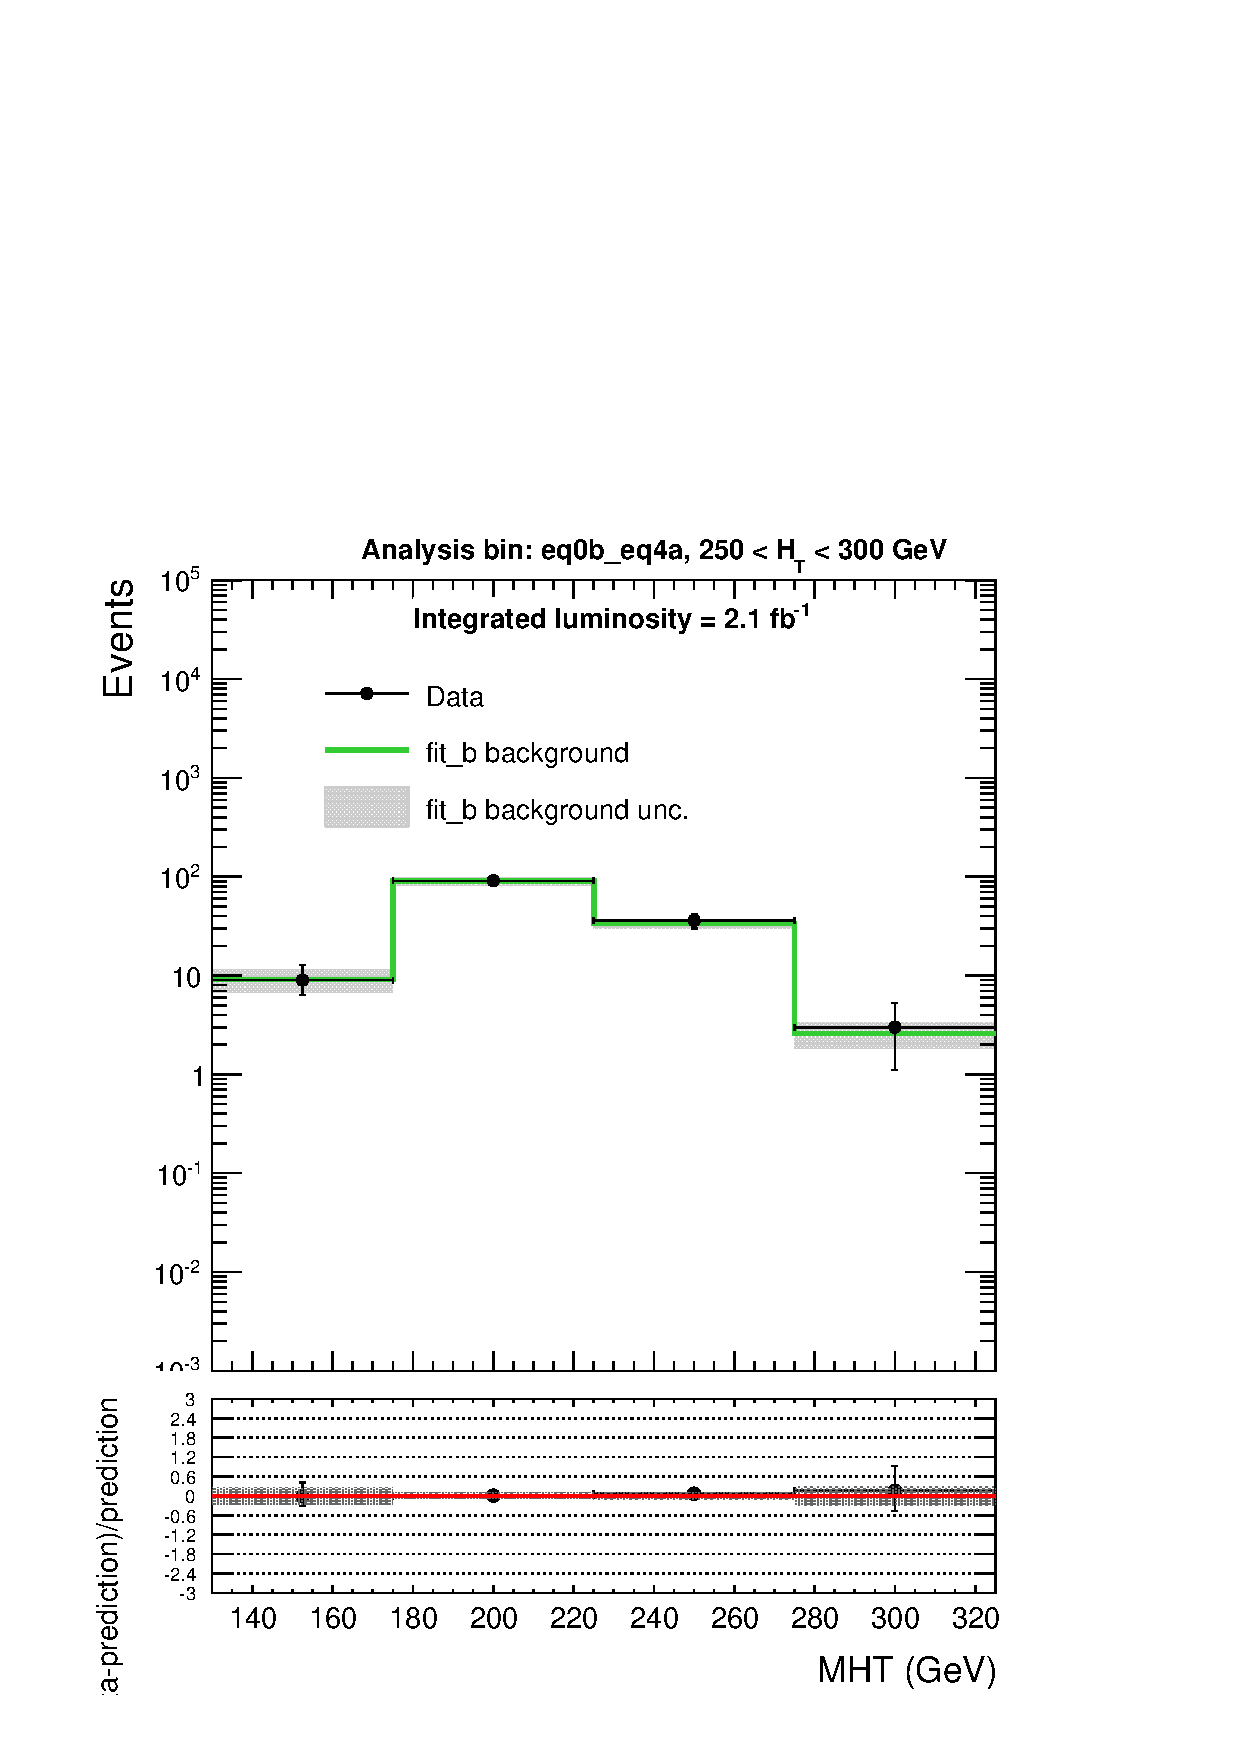
\includegraphics[width=0.25\textwidth]{figures/postFitResults/postFitShapes/postFitShape_eq0b_eq4a_250_300.pdf} }\hspace{1cm}
    \subfigure[$\nj^{\mathrm{asym}}=4$, $\nb=0$, $300 < \scalht < 350 \; \mathrm{GeV}$]{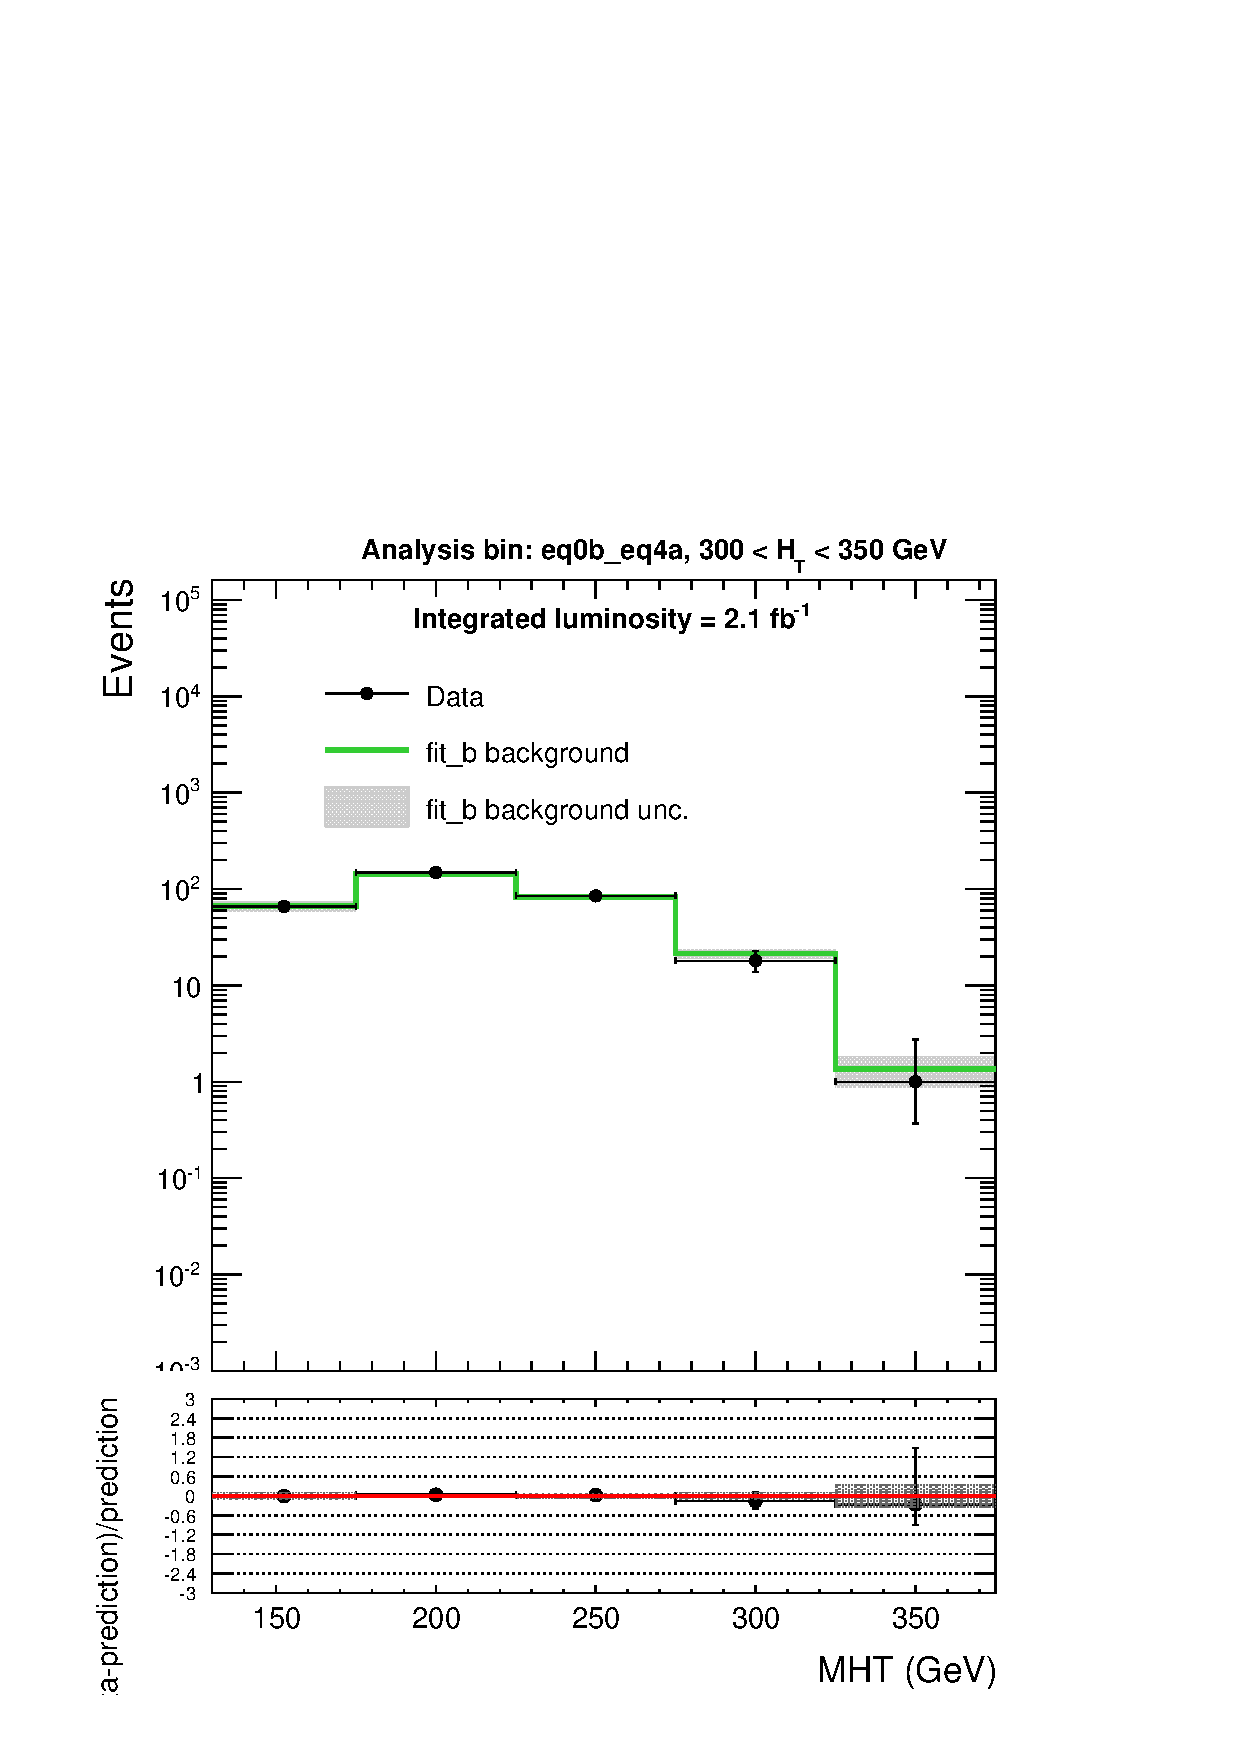
\includegraphics[width=0.25\textwidth]{figures/postFitResults/postFitShapes/postFitShape_eq0b_eq4a_300_350.pdf} }\\
    \subfigure[$\nj^{\mathrm{asym}}=4$, $\nb=0$, $350 < \scalht < 400 \; \mathrm{GeV}$]{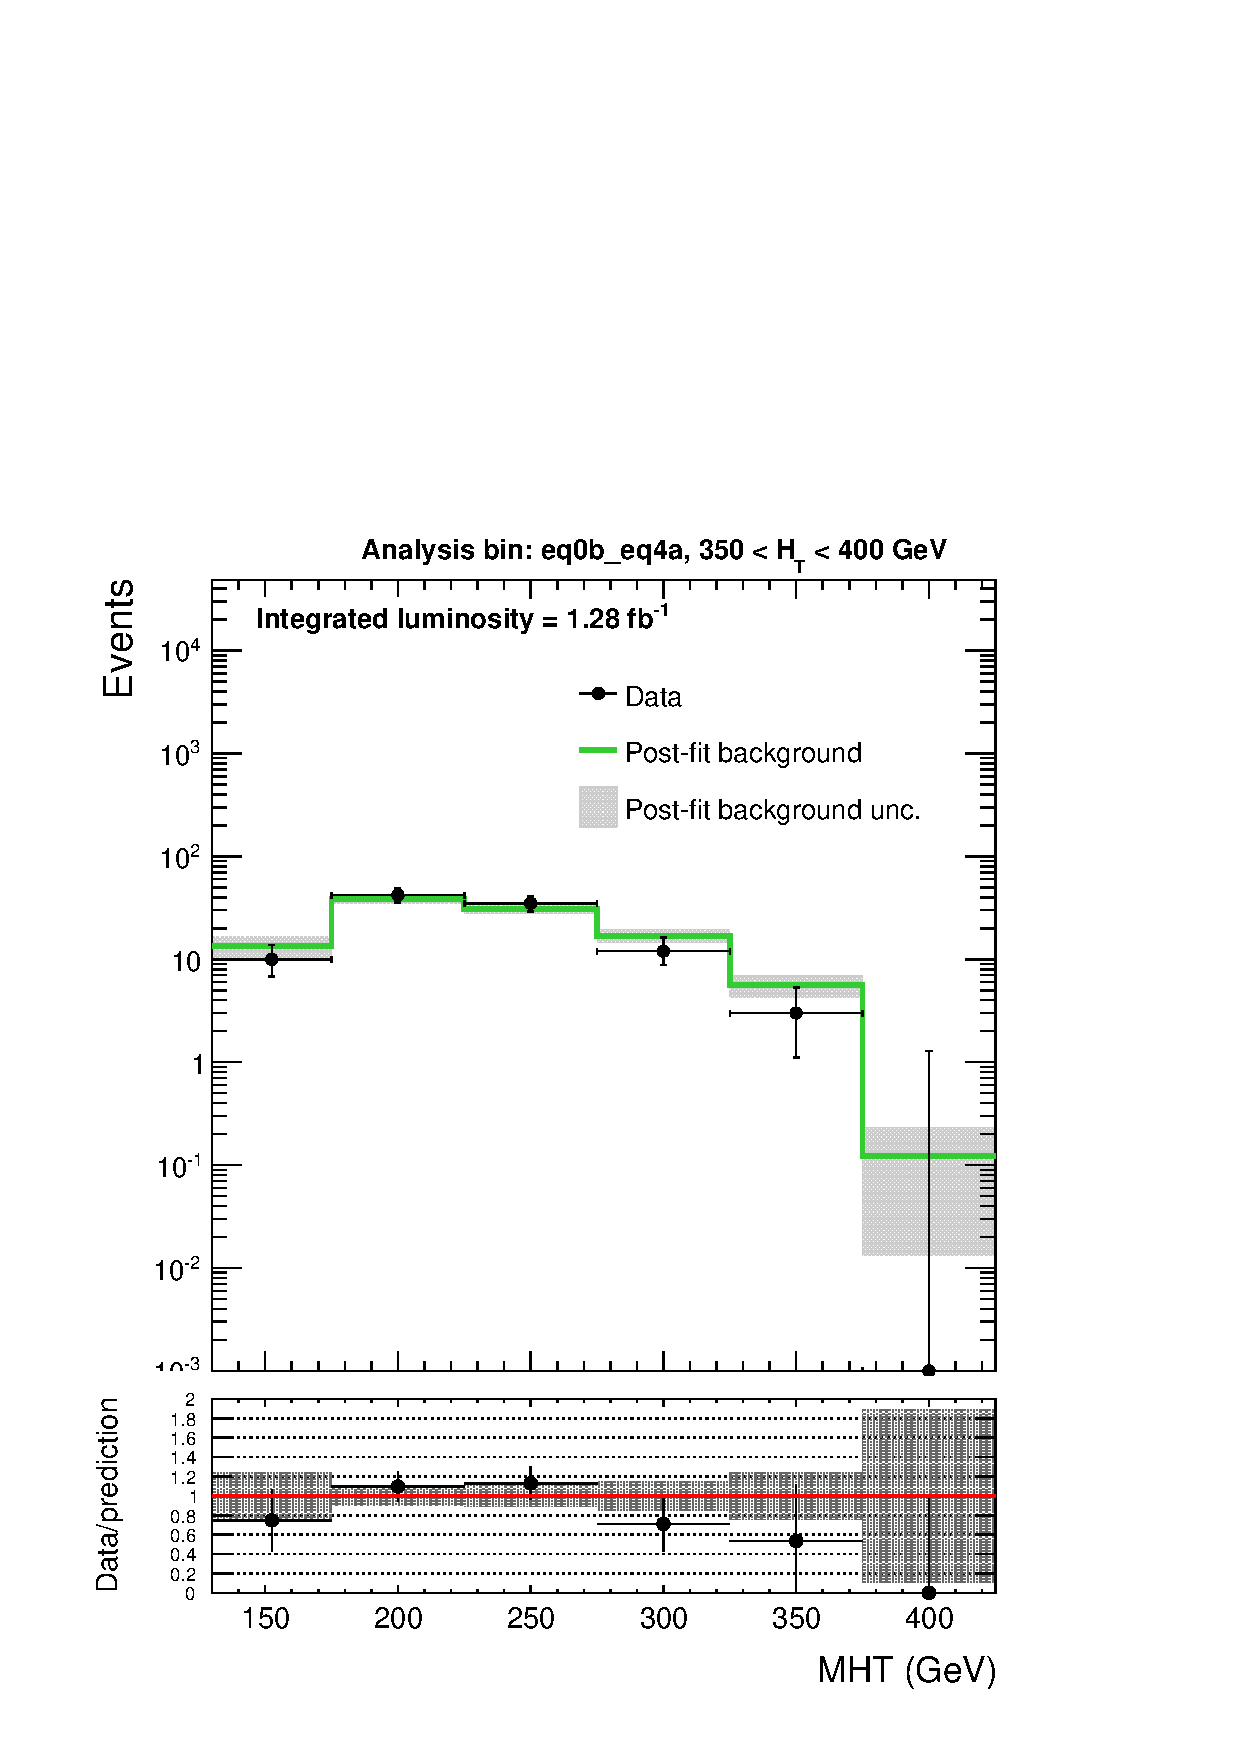
\includegraphics[width=0.25\textwidth]{figures/postFitResults/postFitShapes/postFitShape_eq0b_eq4a_350_400.pdf} }\hspace{1cm}
    \subfigure[$\nj^{\mathrm{asym}}=4$, $\nb=0$, $400 < \scalht < 500 \; \mathrm{GeV}$]{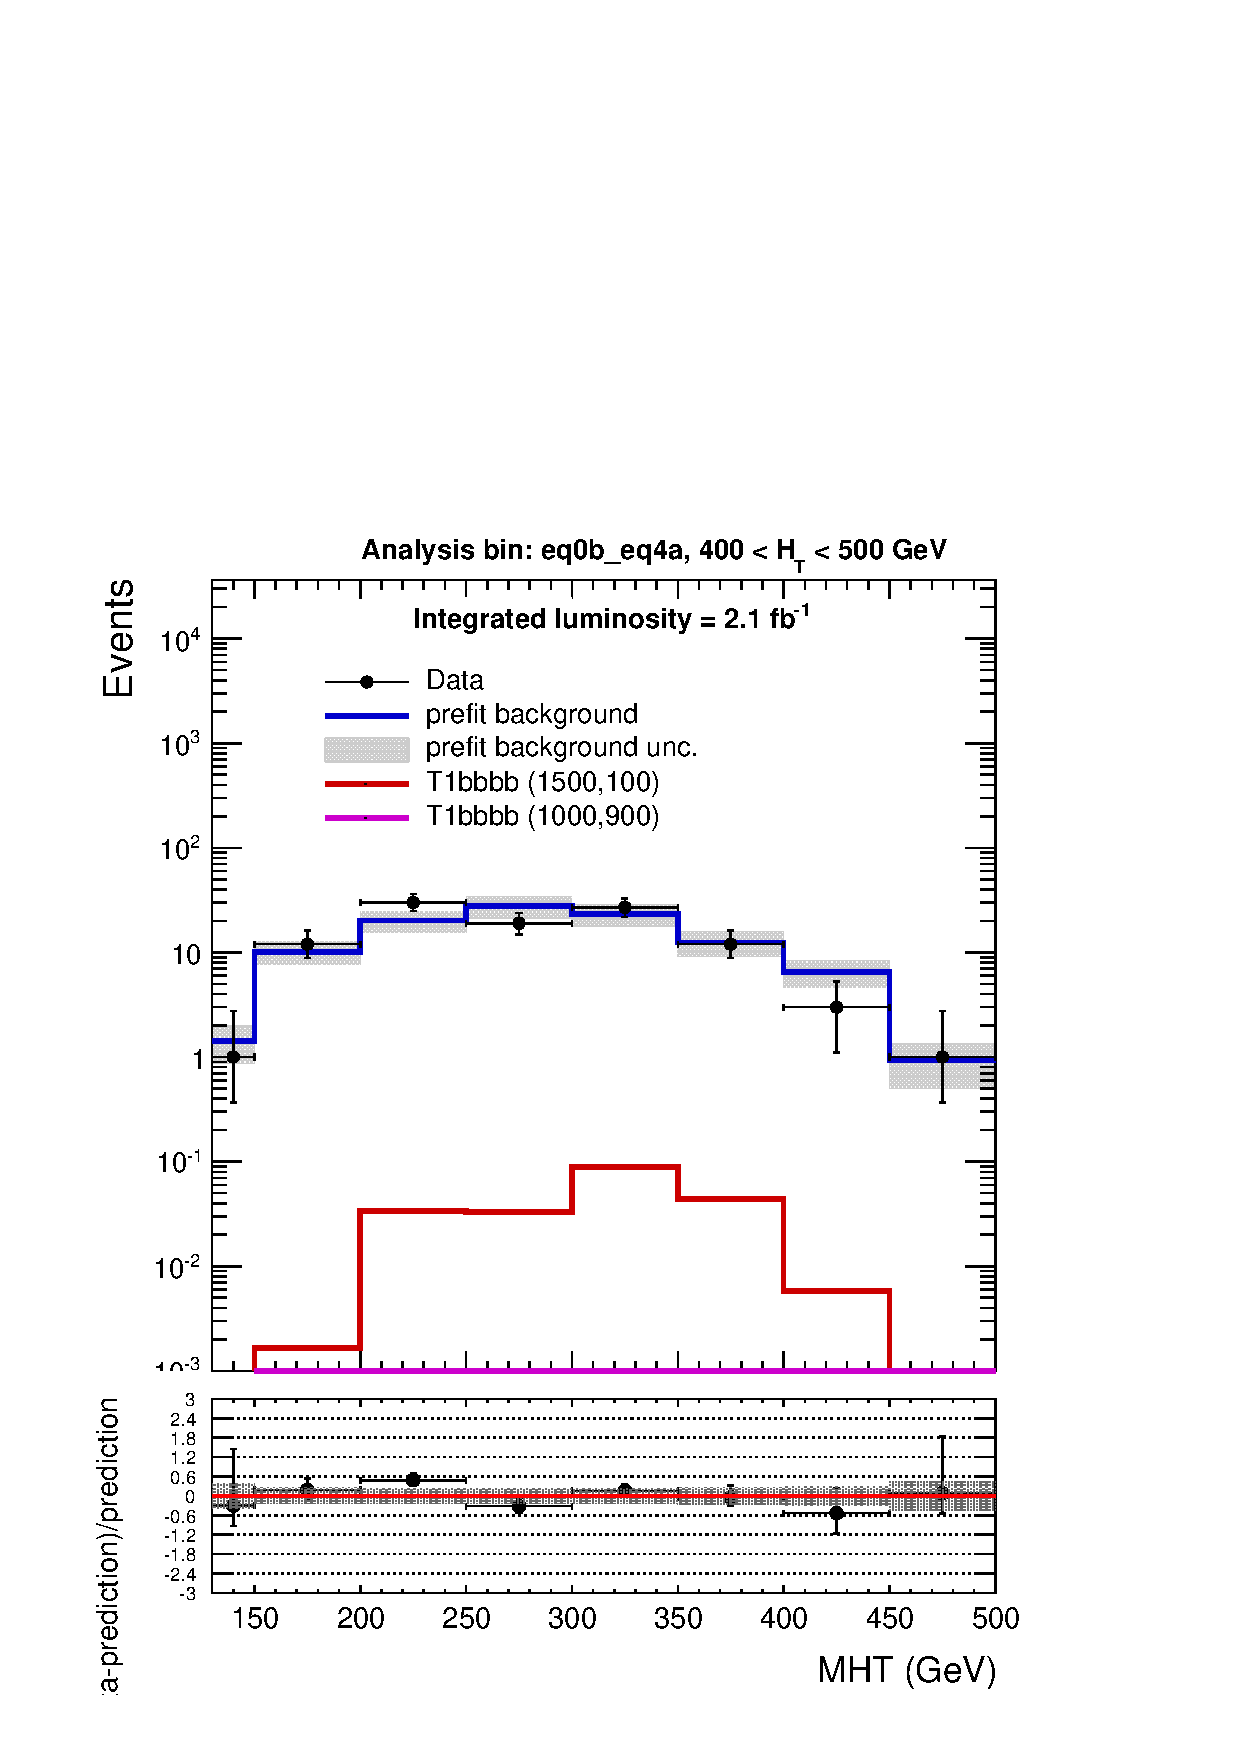
\includegraphics[width=0.25\textwidth]{figures/postFitResults/postFitShapes/postFitShape_eq0b_eq4a_400_500.pdf} }\hspace{1cm}
    \subfigure[$\nj^{\mathrm{asym}}=4$, $\nb=0$, $500 < \scalht < 600 \; \mathrm{GeV}$]{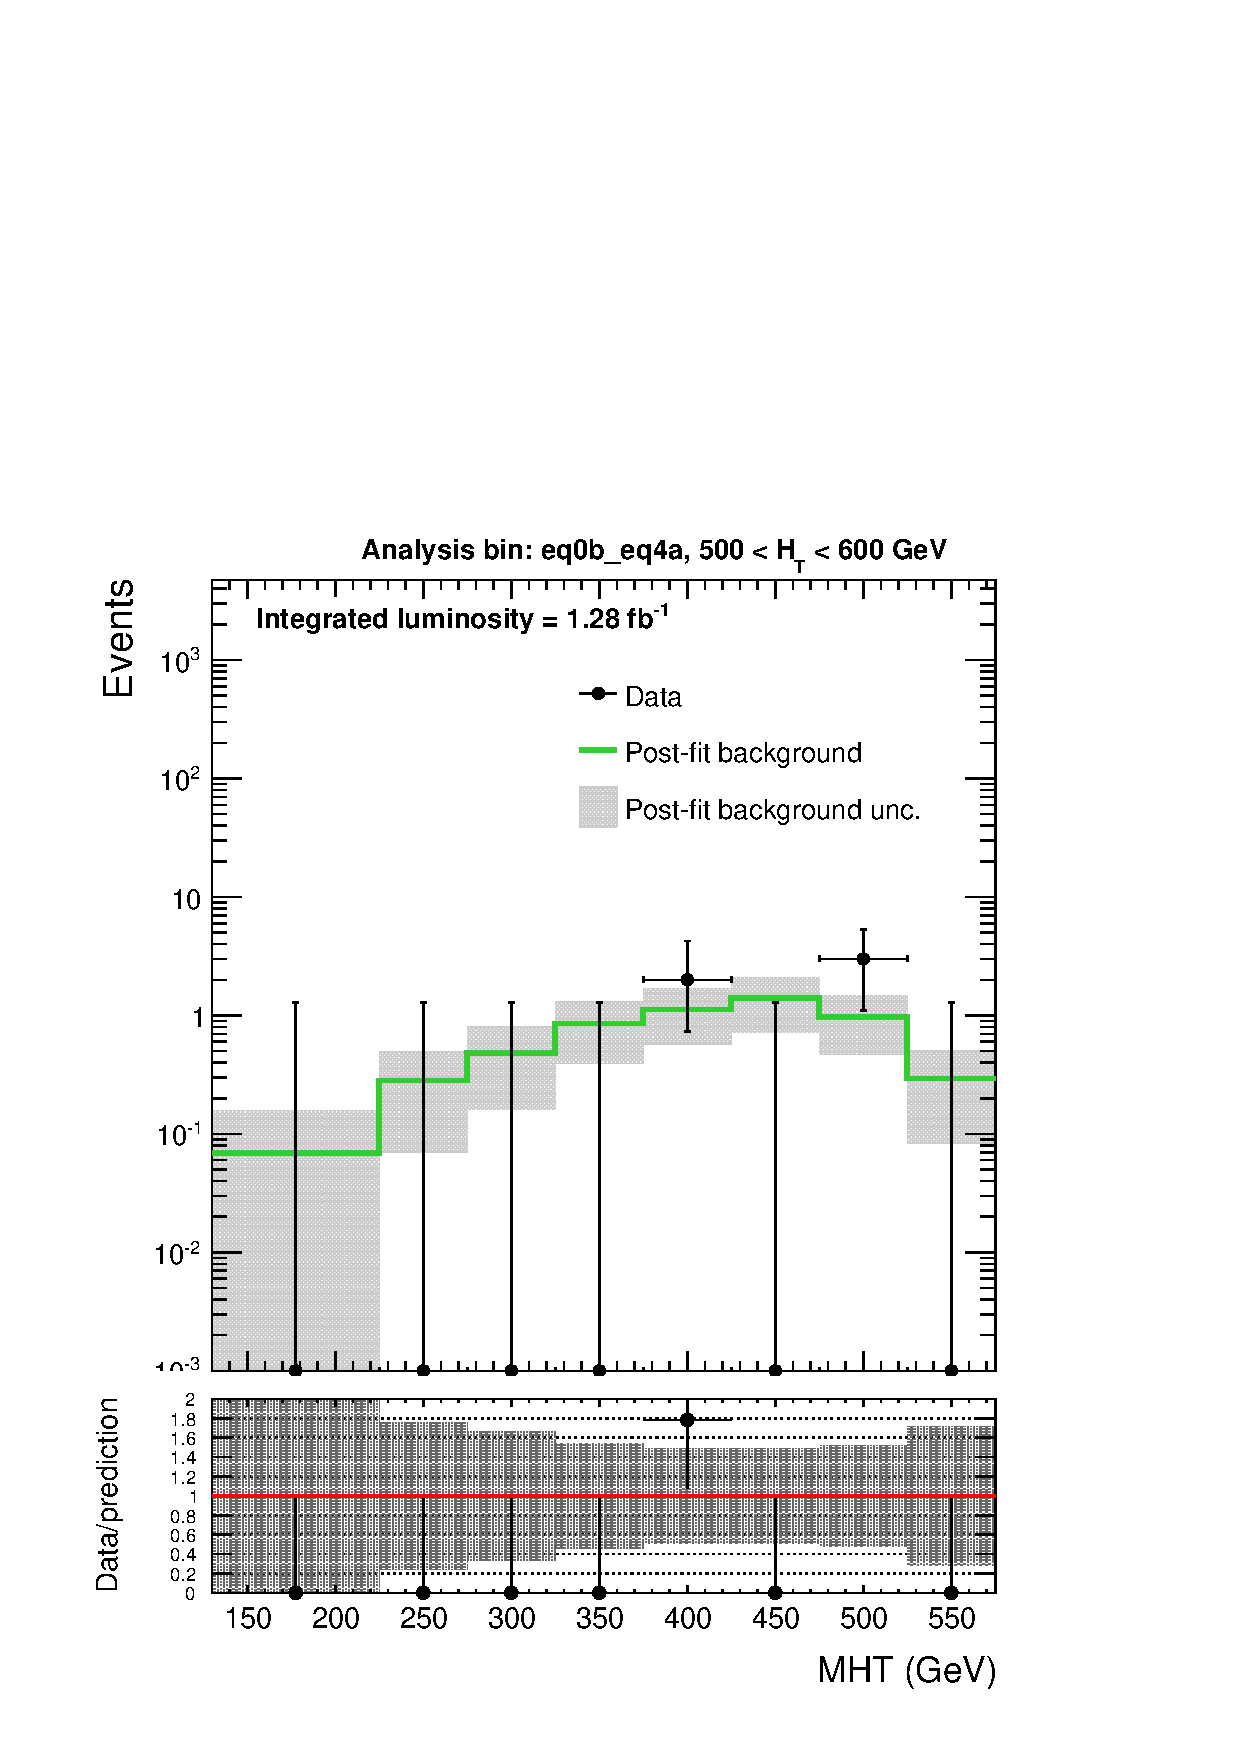
\includegraphics[width=0.25\textwidth]{figures/postFitResults/postFitShapes/postFitShape_eq0b_eq4a_500_600.pdf} }\\
    \subfigure[$\nj^{\mathrm{asym}}=4$, $\nb=0$, $\scalht > 600 \; \mathrm{GeV}$]{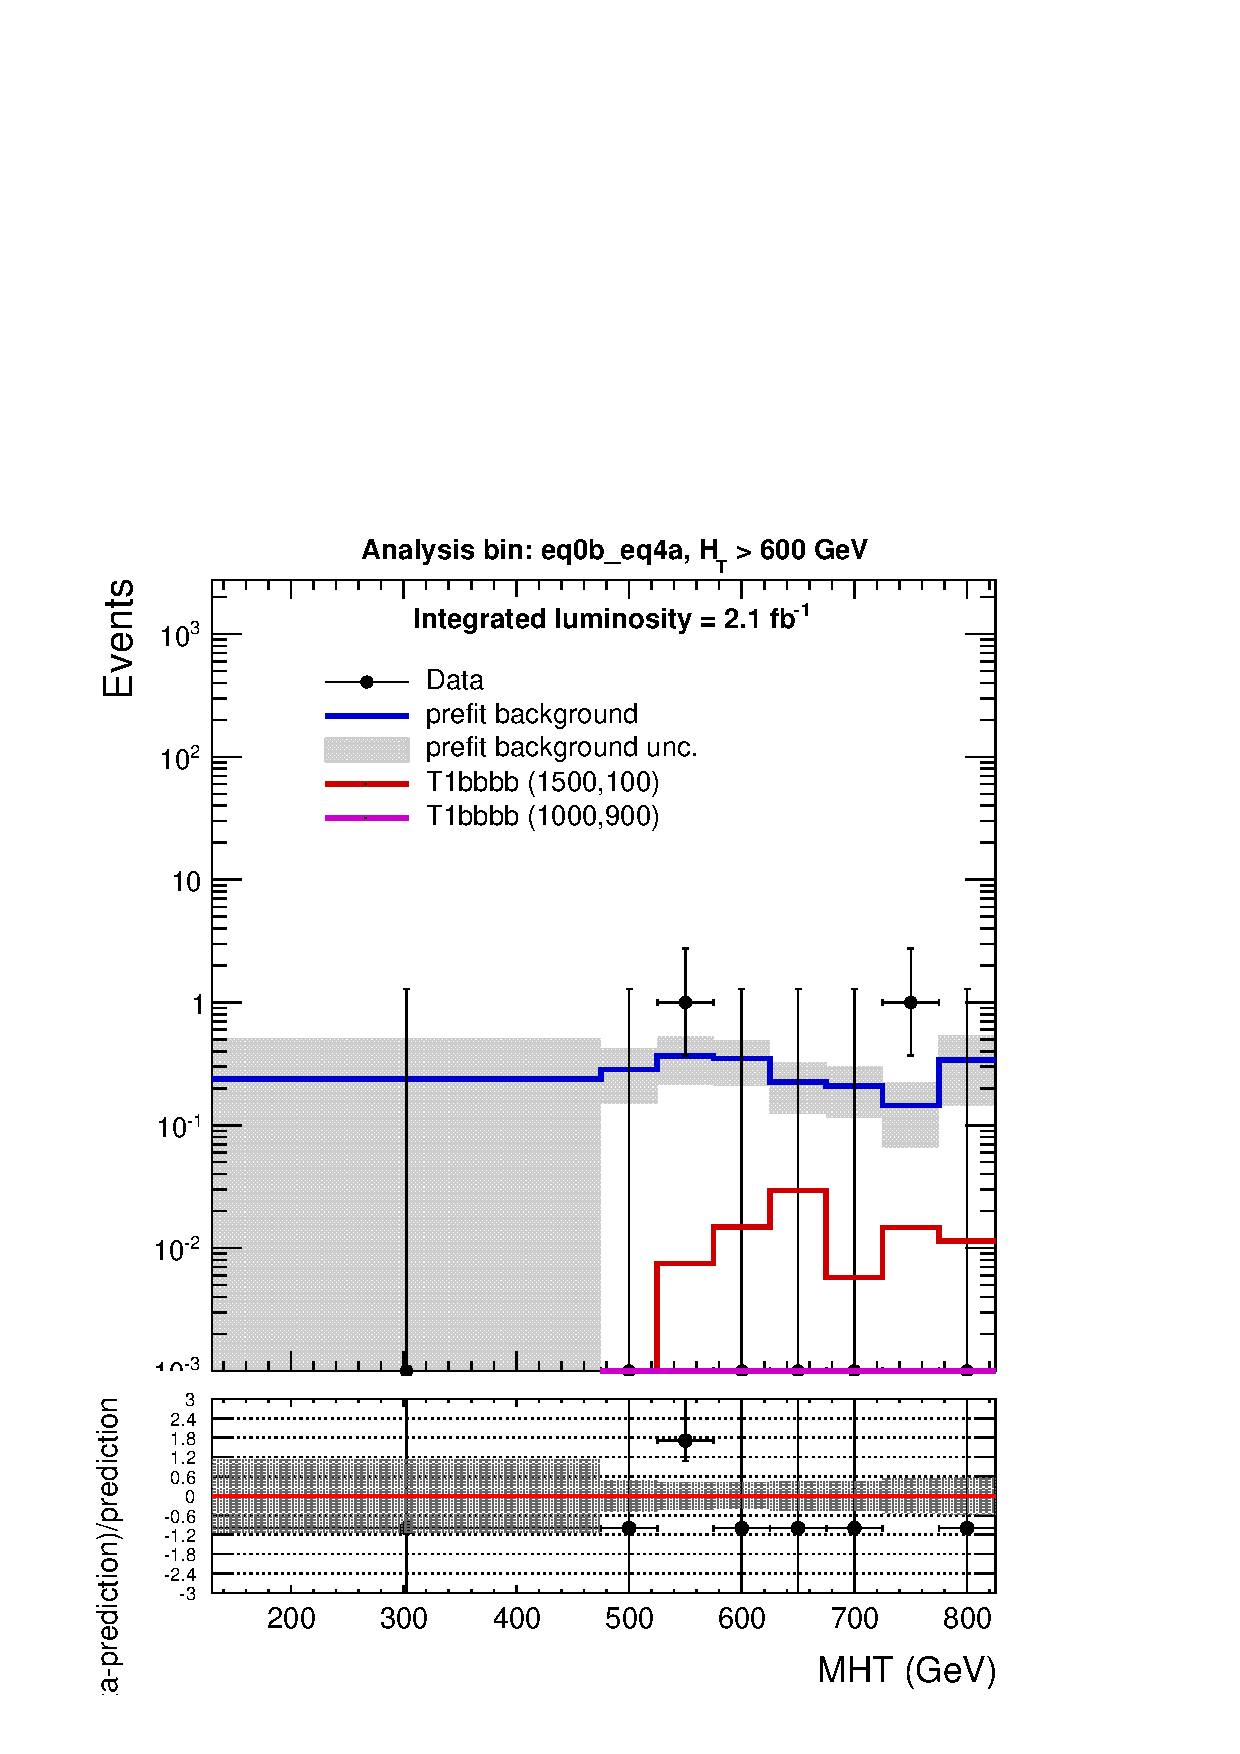
\includegraphics[width=0.25\textwidth]{figures/postFitResults/postFitShapes/postFitShape_eq0b_eq4a_600_Inf.pdf} }\hspace{1cm}
  \end{center}
\end{figure}



\newpage
\begin{figure}[h!]
\caption{Post-fit \MHT templates for the bin $\nj^{\mathrm{sym}}=4$, $\nb=0$ \label{fig:postFitShapes_eq0b_eq4j}}.
\begin{center}

    \subfigure[$\nj^{\mathrm{sym}}=4$, $\nb=0$, $300 < \scalht < 350 \; \mathrm{GeV}$]{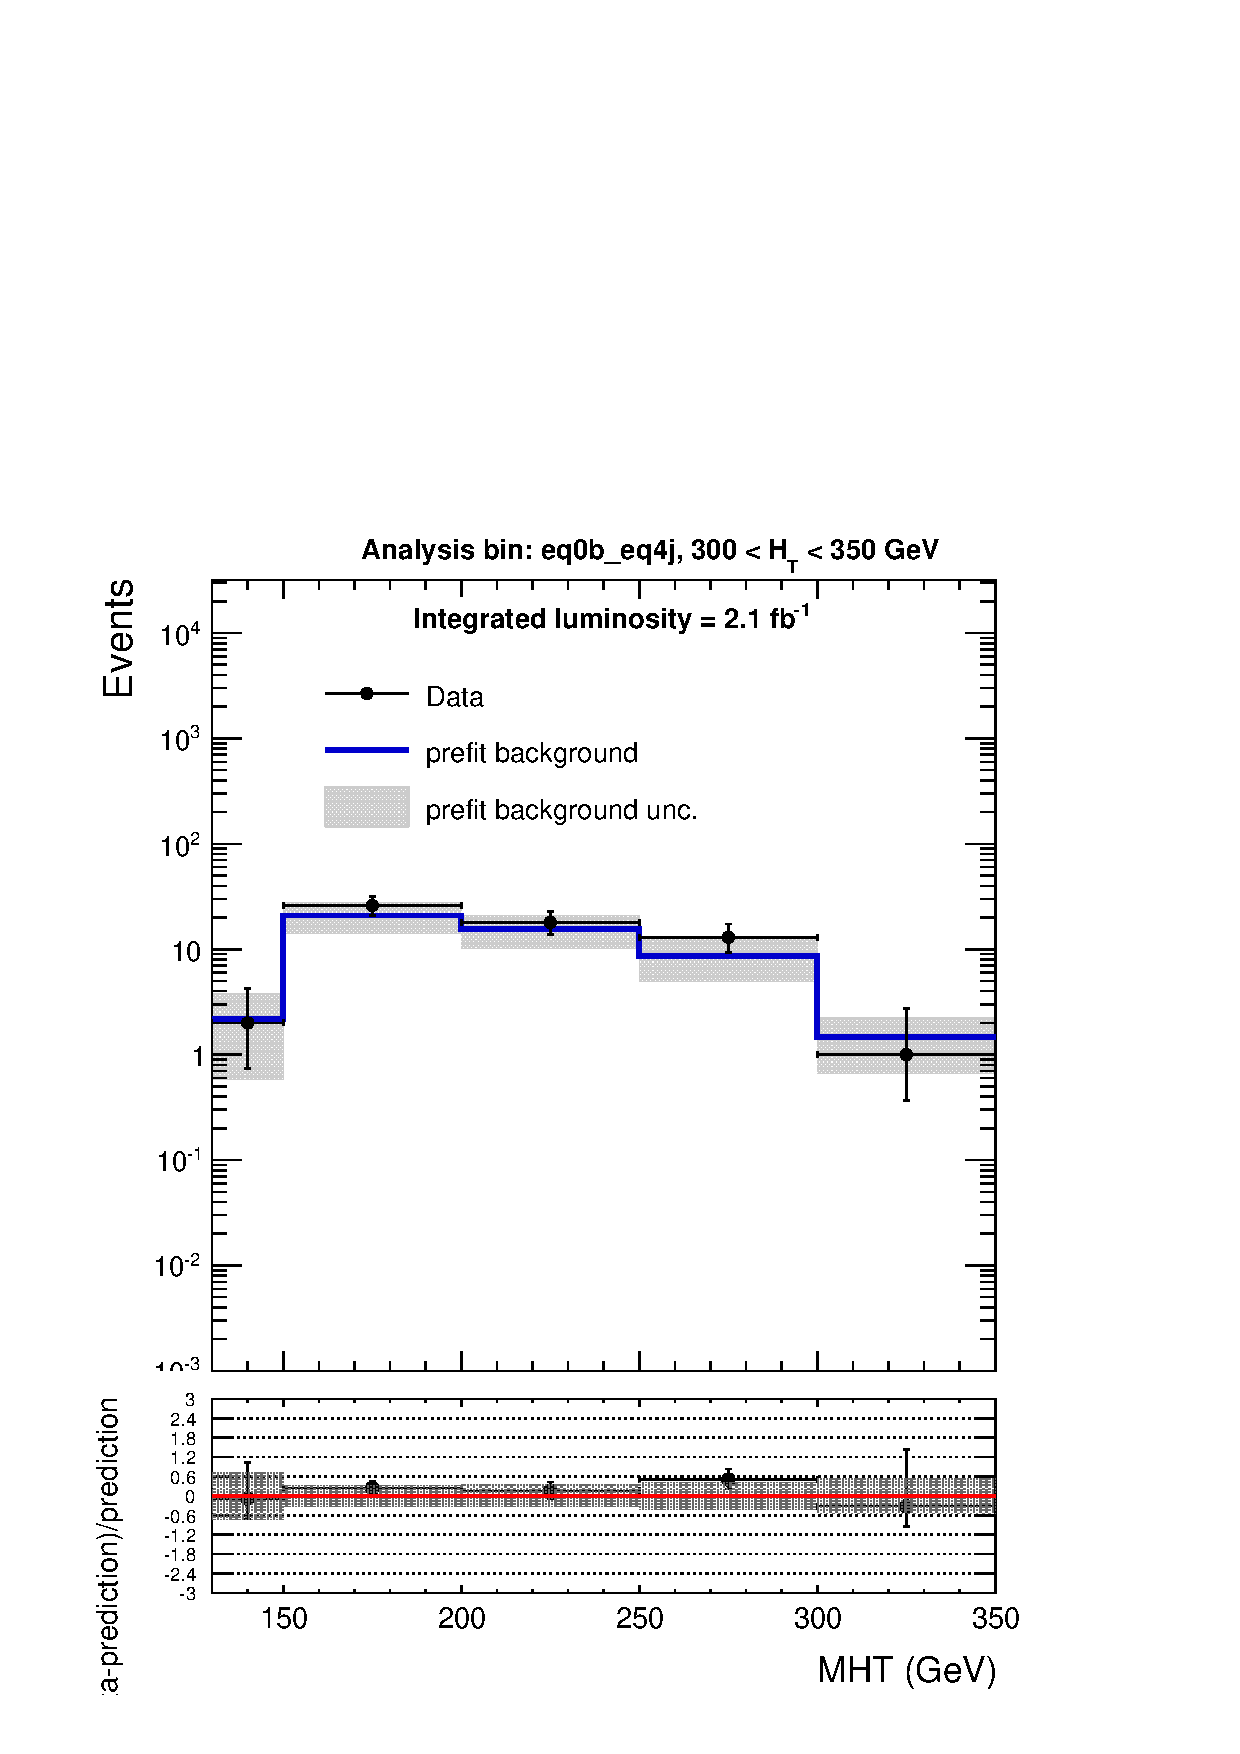
\includegraphics[width=0.25\textwidth]{figures/postFitResults/postFitShapes/postFitShape_eq0b_eq4j_300_350.pdf} }\hspace{1cm}
    \subfigure[$\nj^{\mathrm{sym}}=4$, $\nb=0$, $350 < \scalht < 400 \; \mathrm{GeV}$]{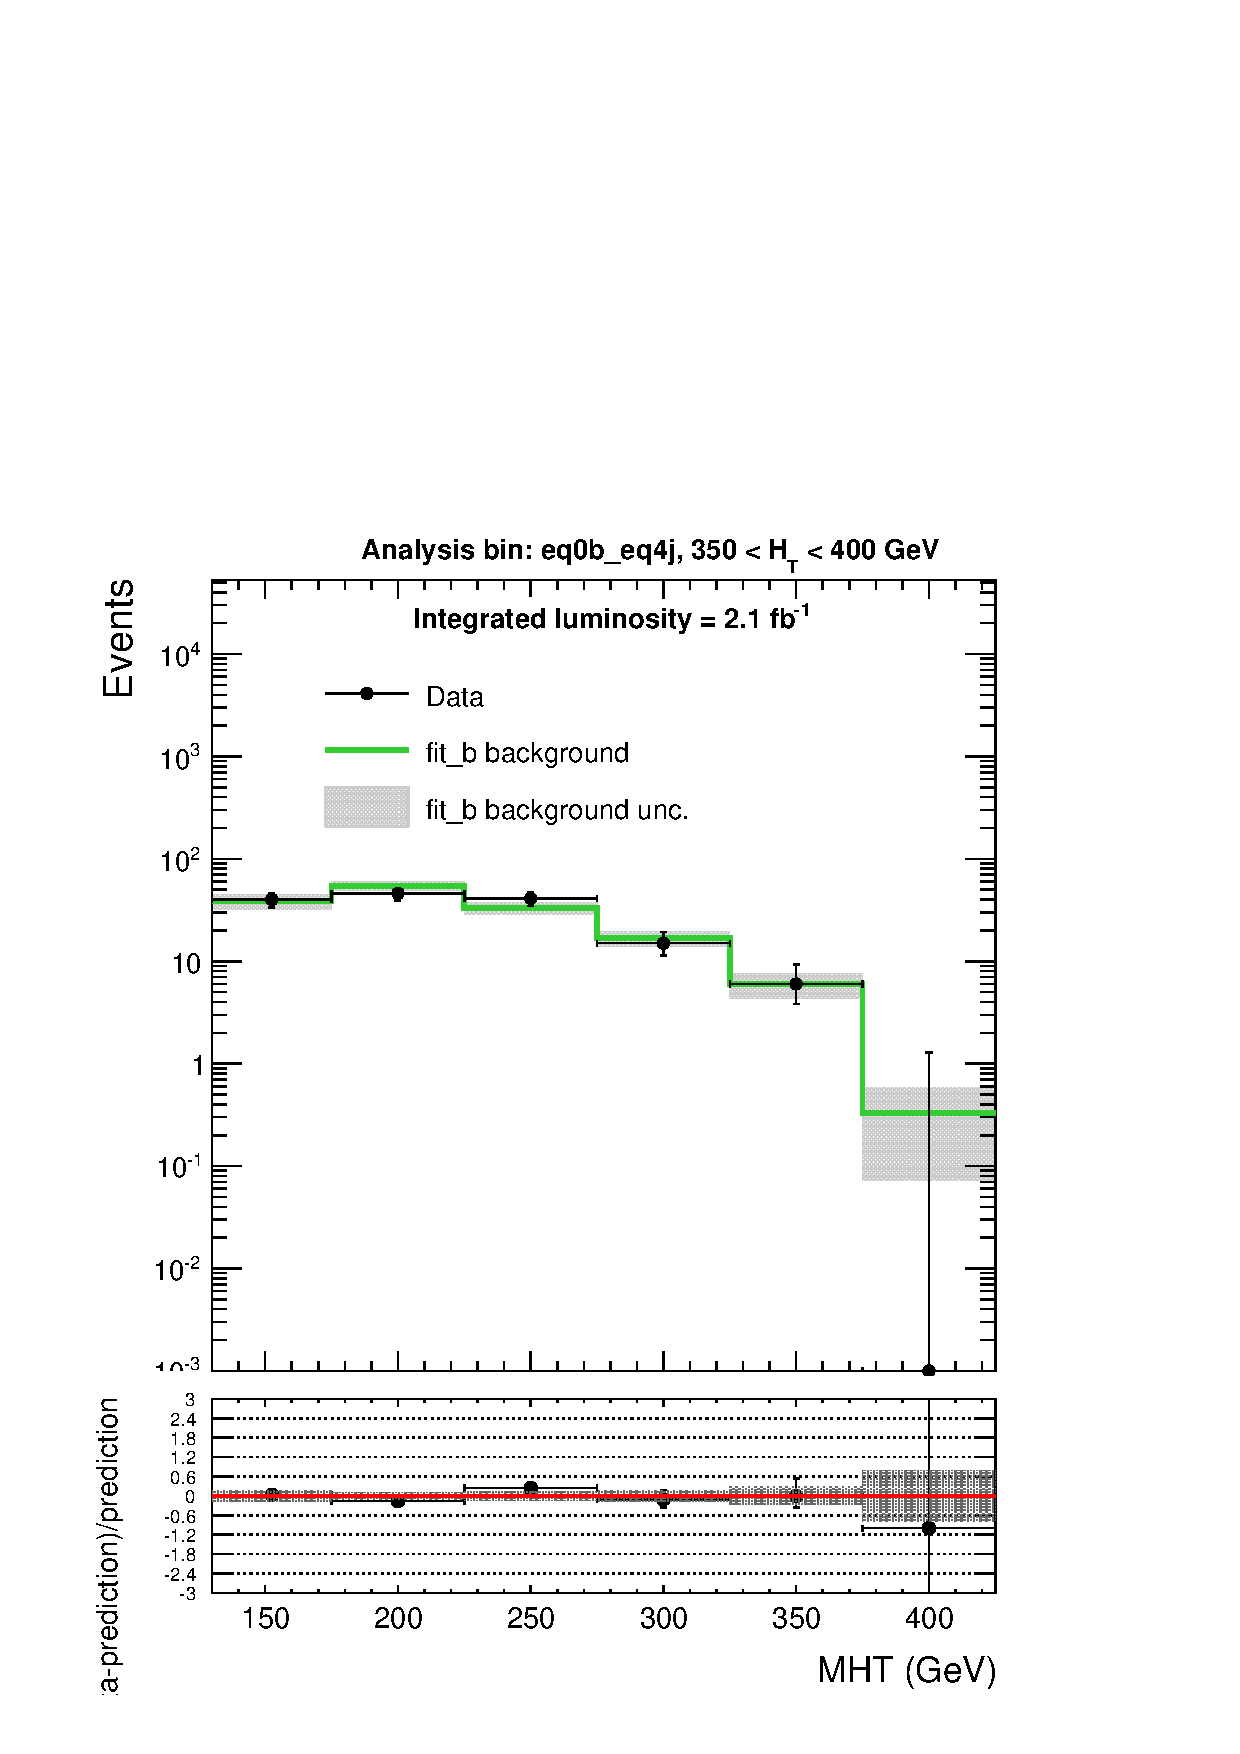
\includegraphics[width=0.25\textwidth]{figures/postFitResults/postFitShapes/postFitShape_eq0b_eq4j_350_400.pdf} }\hspace{1cm}
    \subfigure[$\nj^{\mathrm{sym}}=4$, $\nb=0$, $400 < \scalht < 500 \; \mathrm{GeV}$]{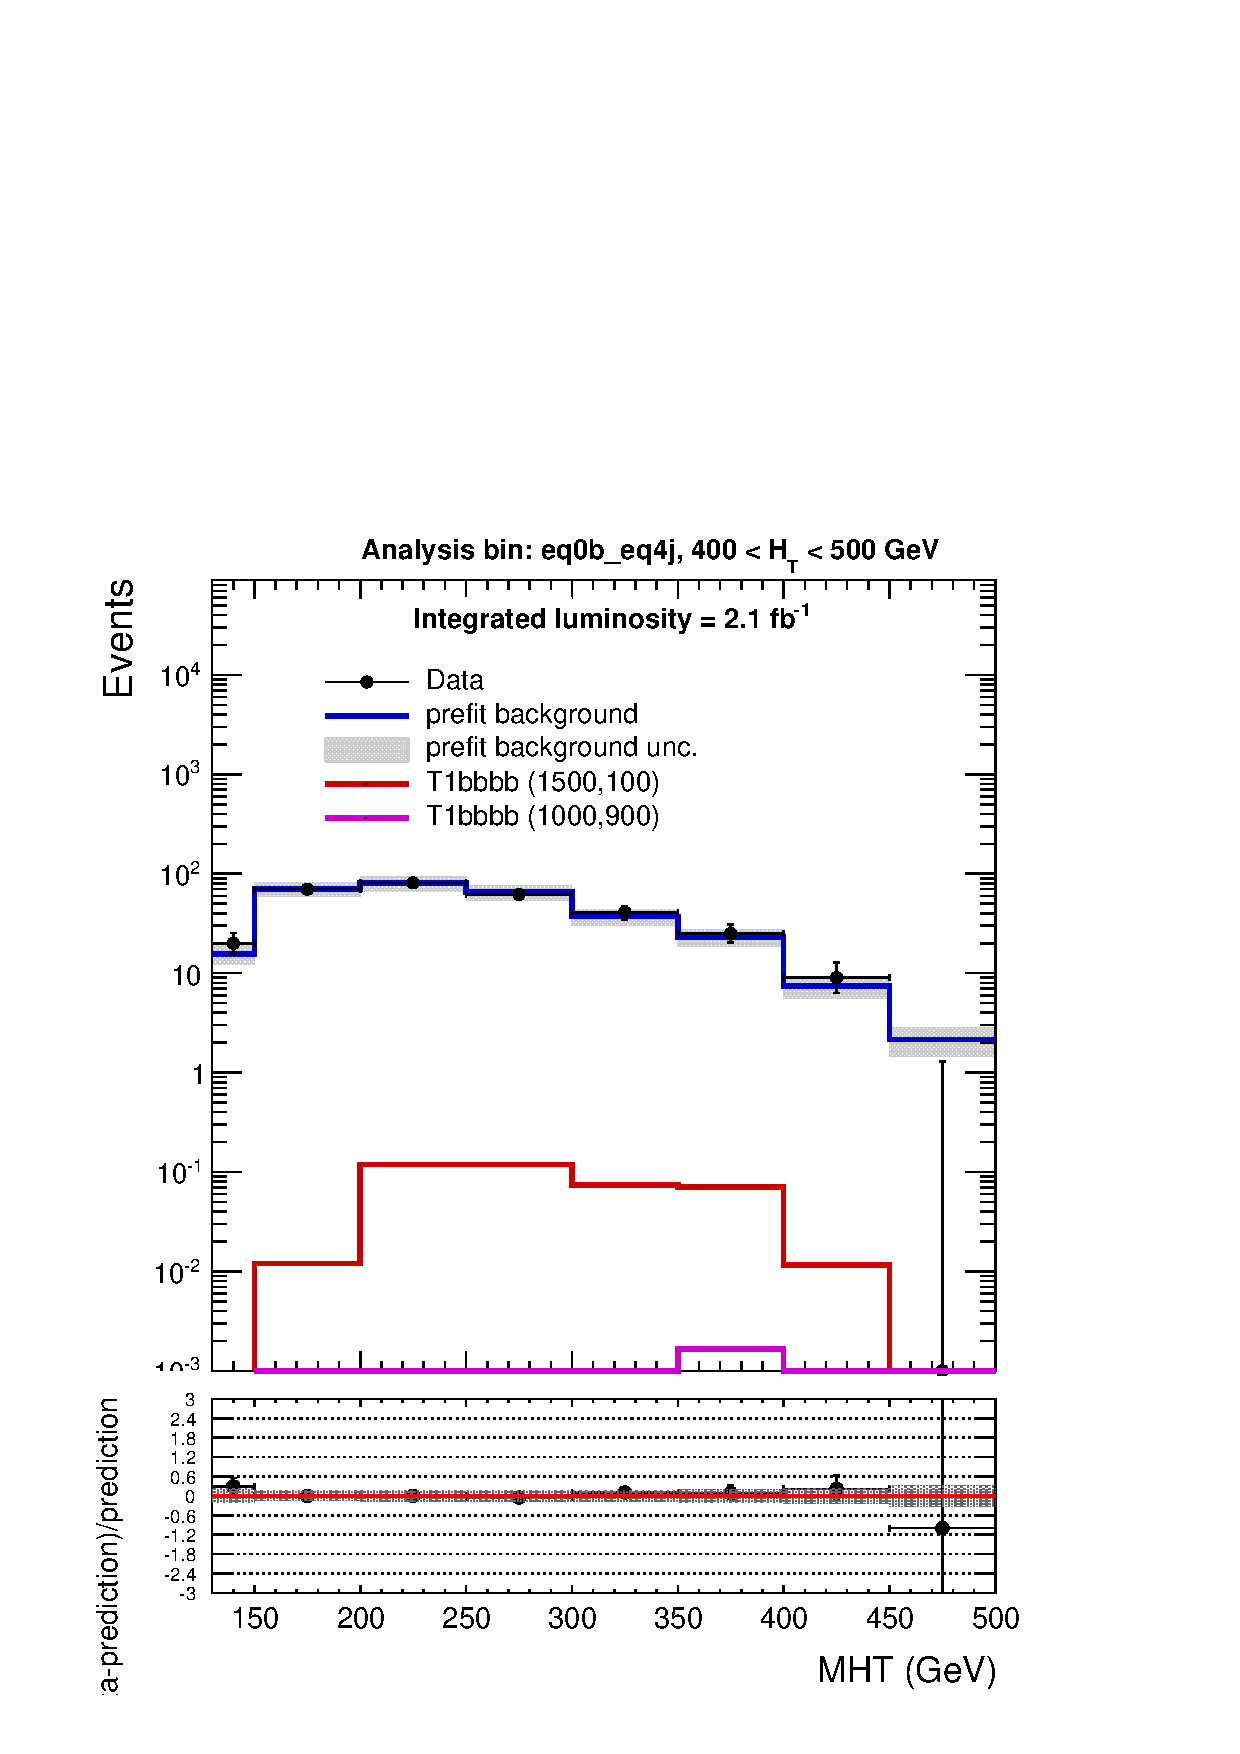
\includegraphics[width=0.25\textwidth]{figures/postFitResults/postFitShapes/postFitShape_eq0b_eq4j_400_500.pdf} }\\
    \subfigure[$\nj^{\mathrm{sym}}=4$, $\nb=0$, $500 < \scalht < 600 \; \mathrm{GeV}$]{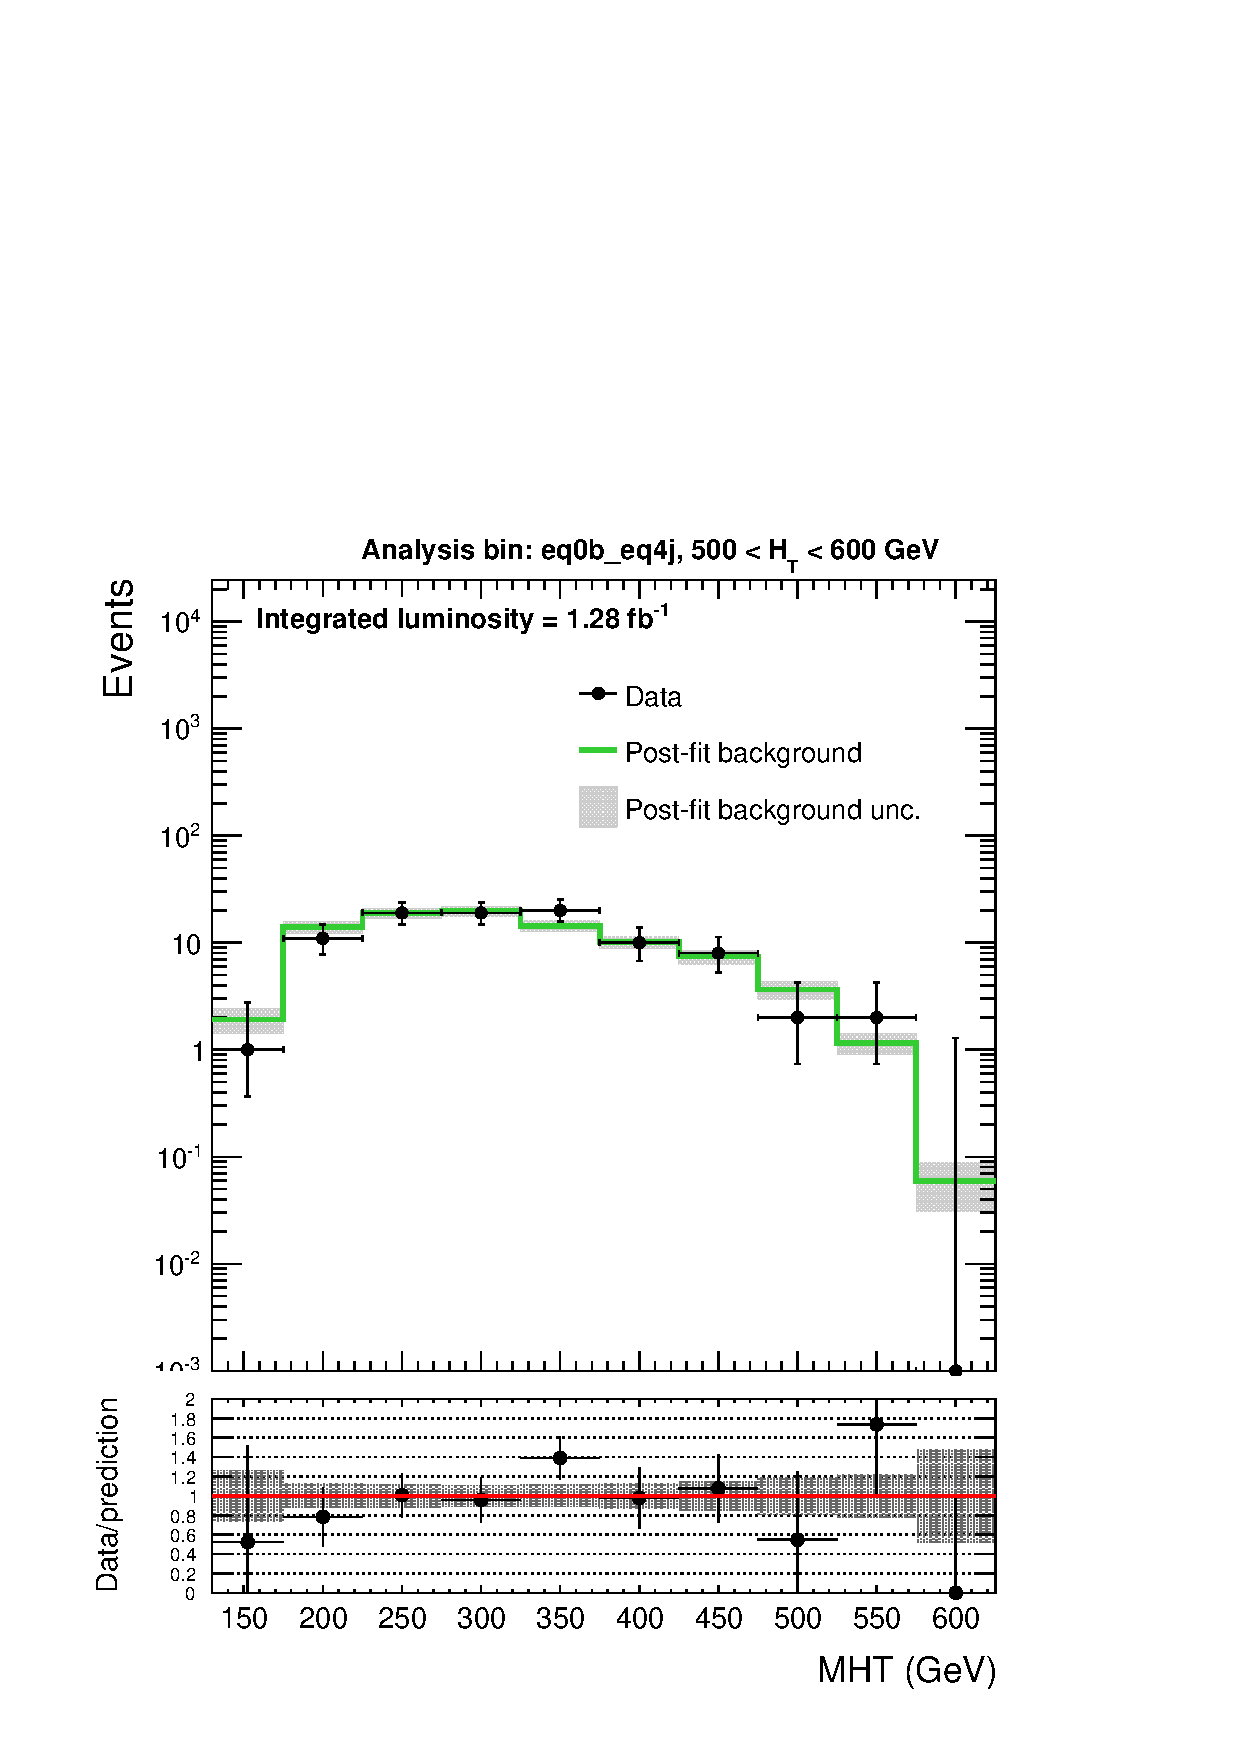
\includegraphics[width=0.25\textwidth]{figures/postFitResults/postFitShapes/postFitShape_eq0b_eq4j_500_600.pdf} }\hspace{1cm}
    \subfigure[$\nj^{\mathrm{sym}}=4$, $\nb=0$, $600 < \scalht < 800 \; \mathrm{GeV}$]{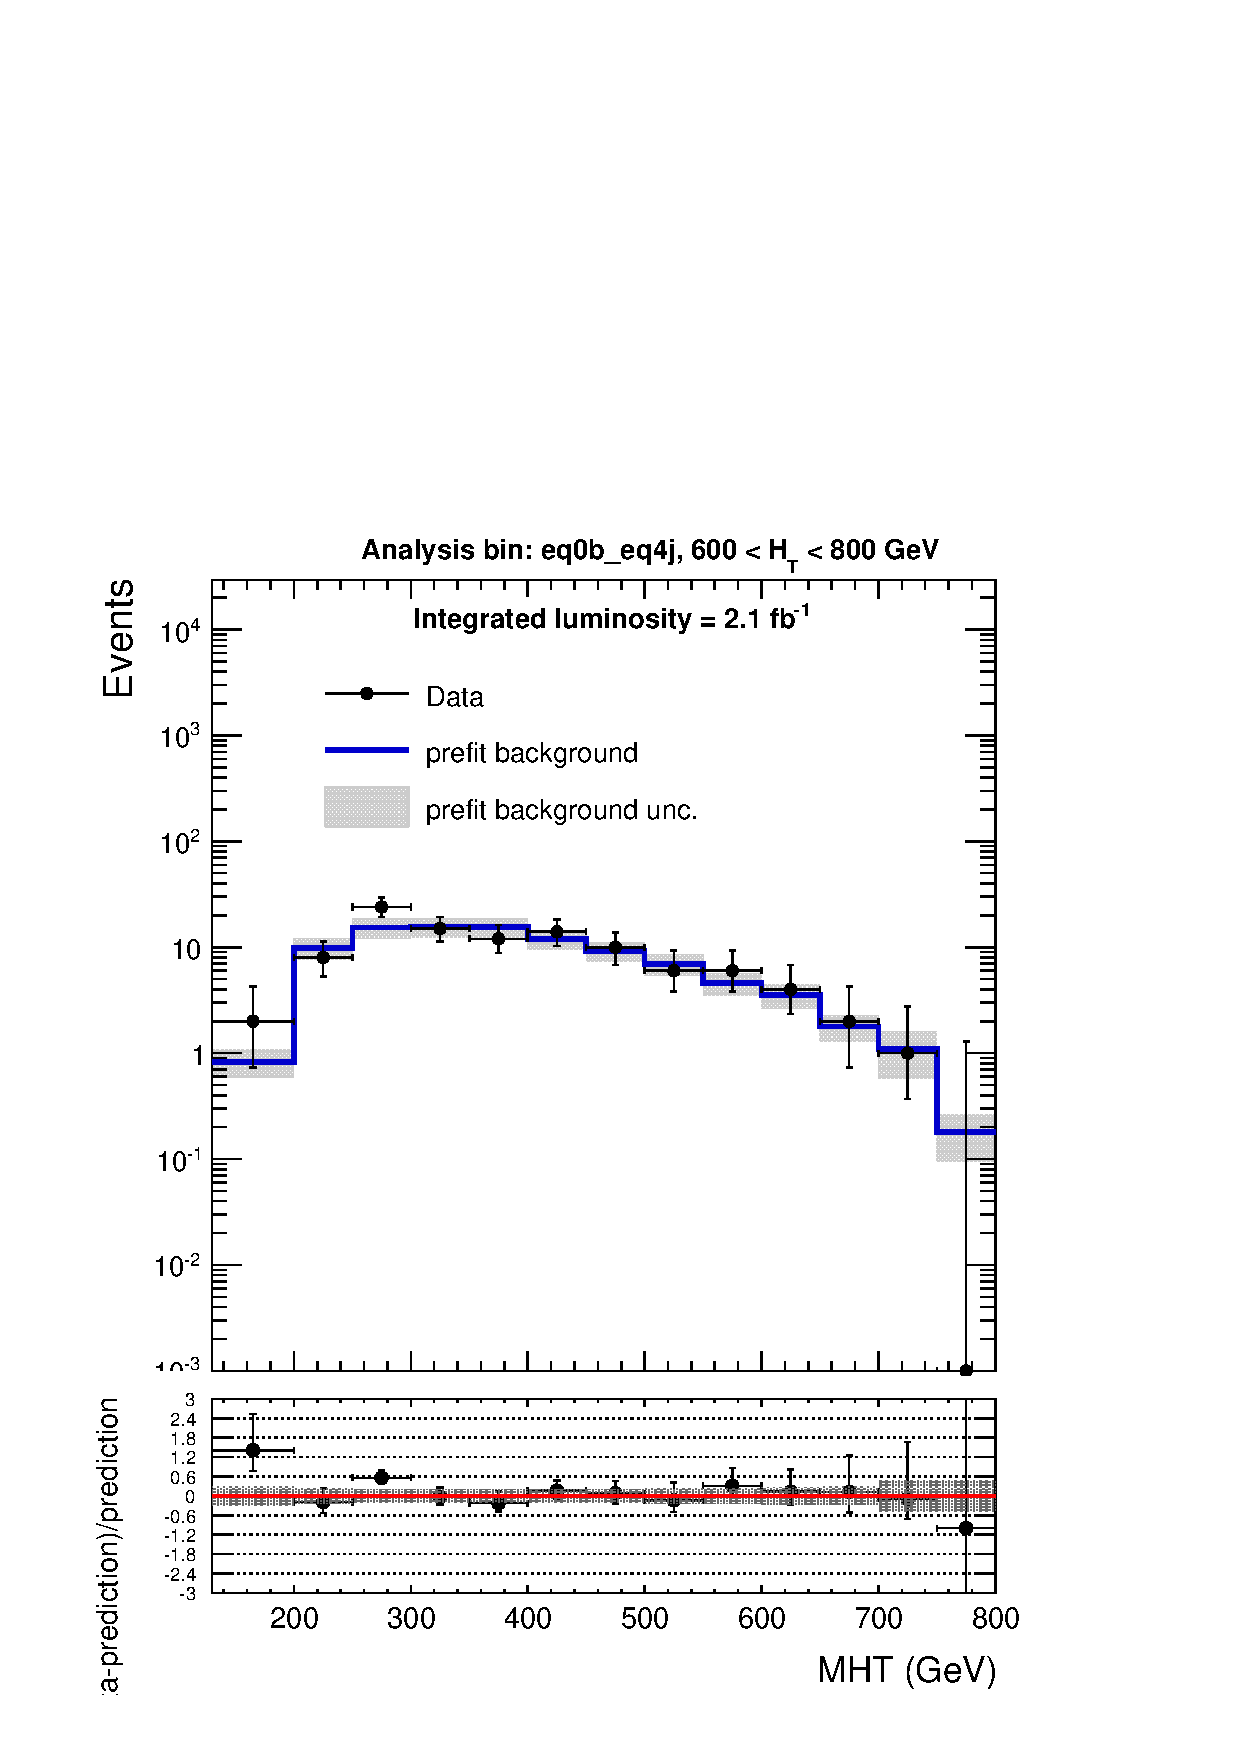
\includegraphics[width=0.25\textwidth]{figures/postFitResults/postFitShapes/postFitShape_eq0b_eq4j_600_800.pdf} }\hspace{1cm}
    \subfigure[$\nj^{\mathrm{sym}}=4$, $\nb=0$, $\scalht > 800 \; \mathrm{GeV}$]{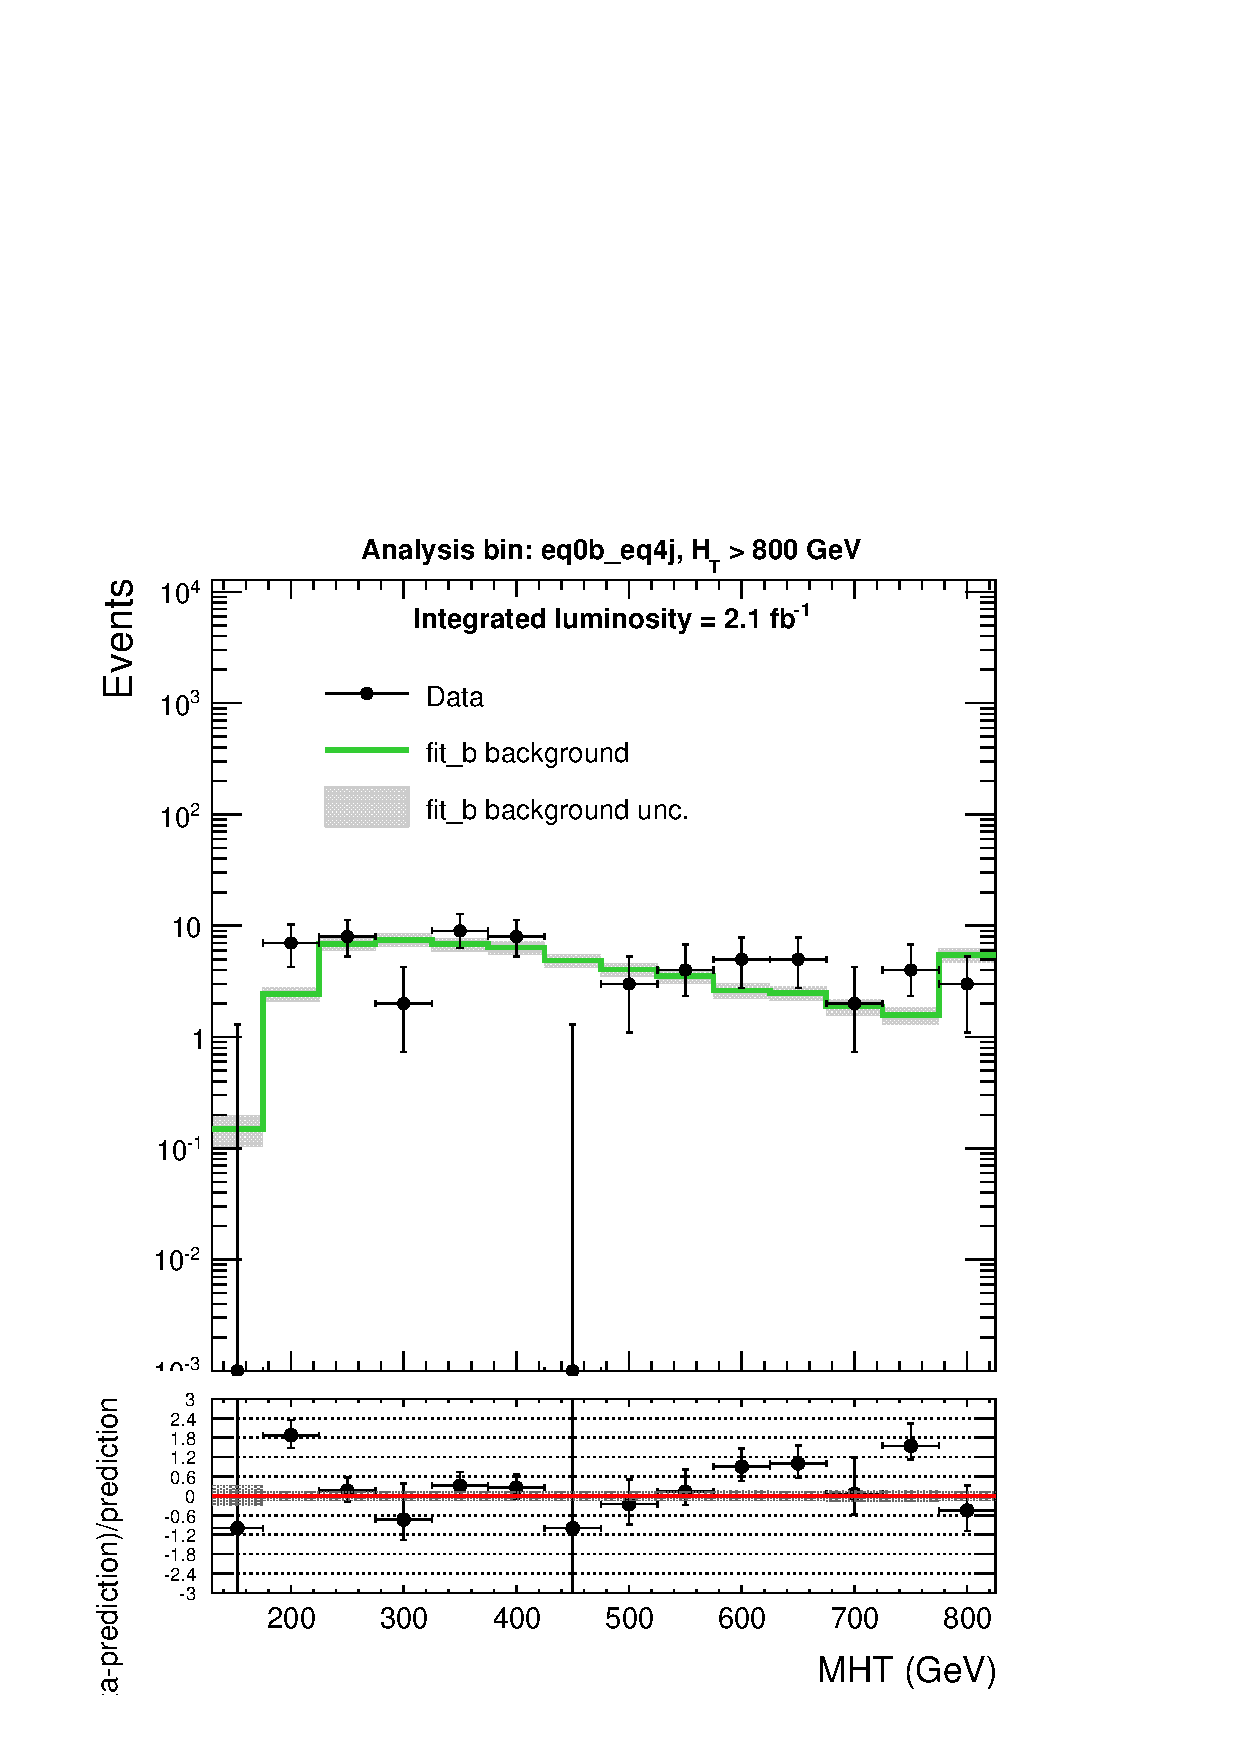
\includegraphics[width=0.25\textwidth]{figures/postFitResults/postFitShapes/postFitShape_eq0b_eq4j_800_Inf.pdf} }\\
  \end{center}
\end{figure}



\newpage
\begin{figure}[h!]
\caption{Post-fit \MHT templates for the bin $\nj^{\mathrm{asym}}=5$, $\nb=0$ \label{fig:postFitShapes_eq0b_ge5a}}.
\begin{center}

    \subfigure[$\nj^{\mathrm{asym}}=5$, $\nb=0$, $300 < \scalht < 350 \; \mathrm{GeV}$]{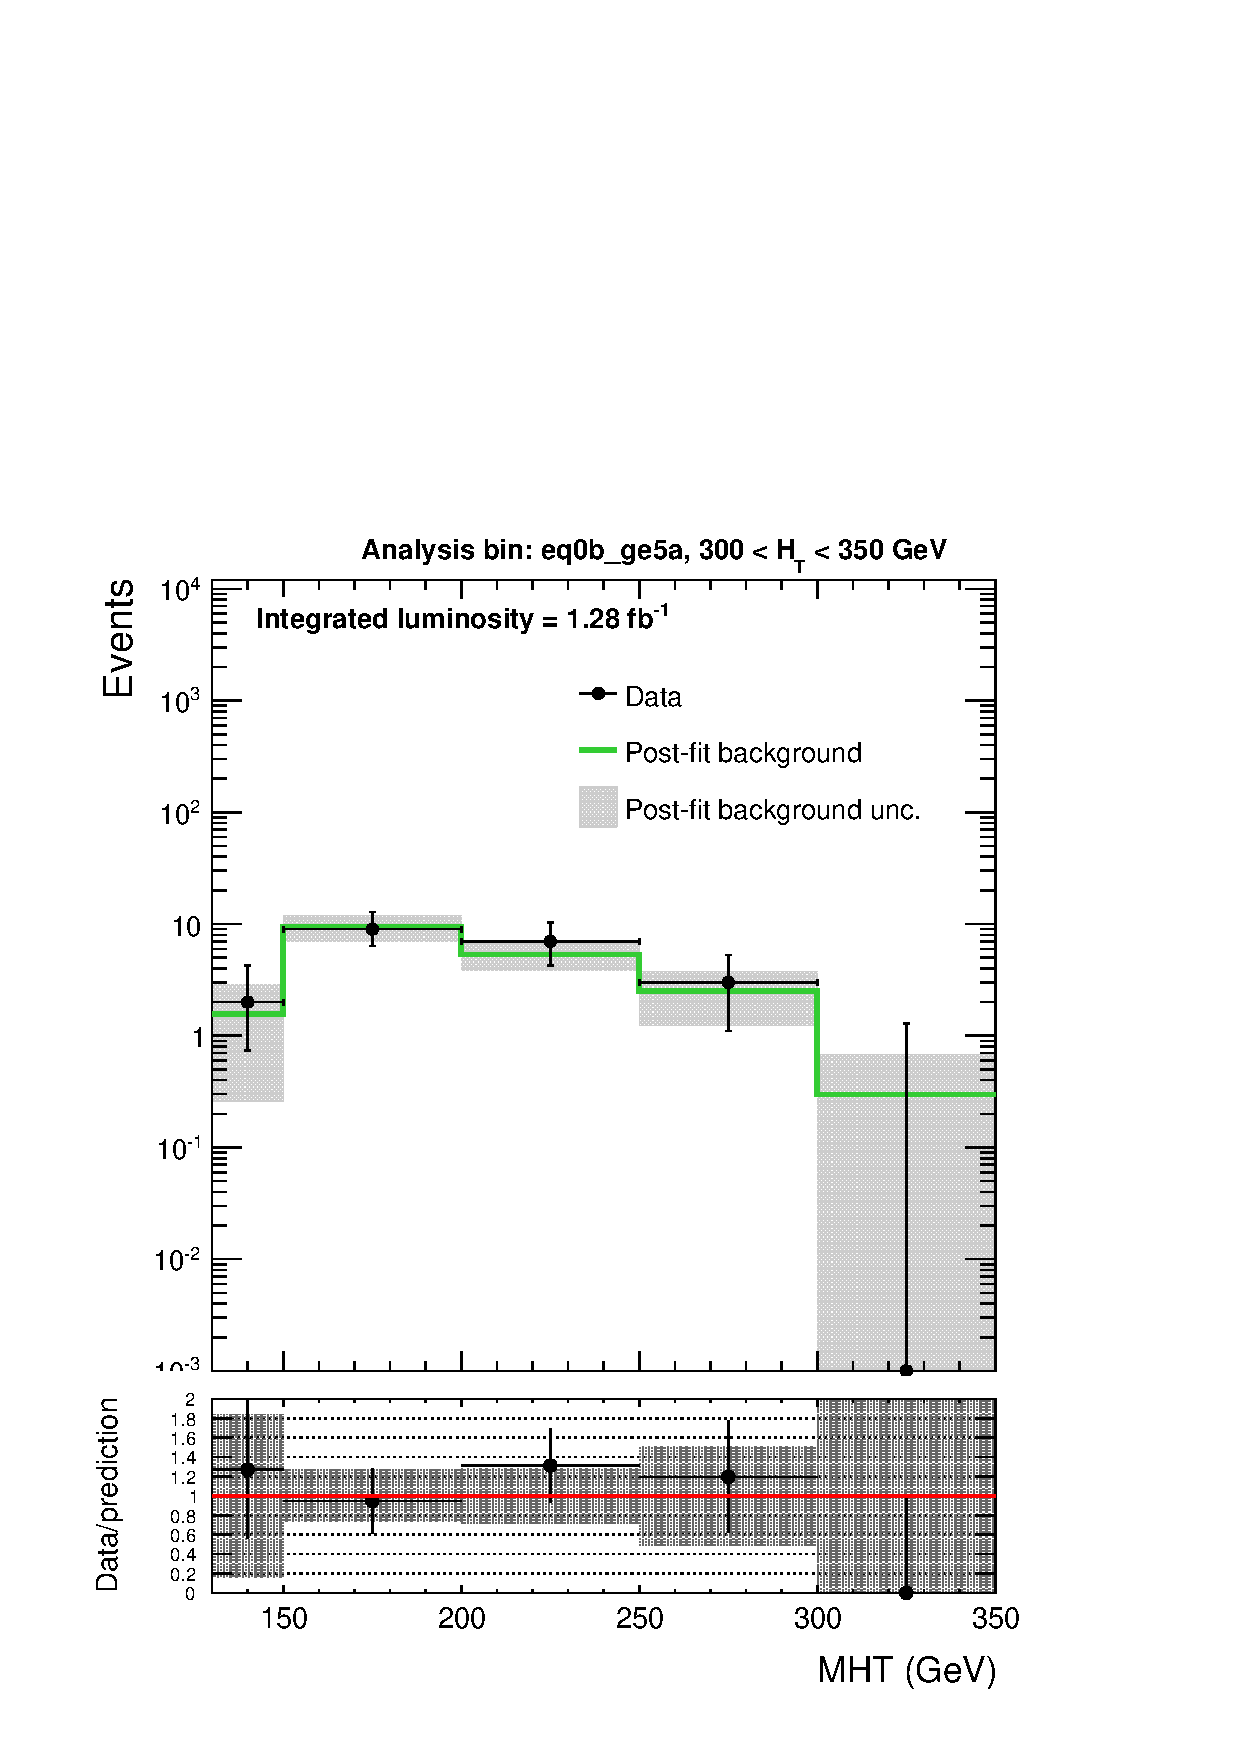
\includegraphics[width=0.25\textwidth]{figures/postFitResults/postFitShapes/postFitShape_eq0b_ge5a_300_350.pdf} }\hspace{1cm}
    \subfigure[$\nj^{\mathrm{asym}}=5$, $\nb=0$, $350 < \scalht < 400 \; \mathrm{GeV}$]{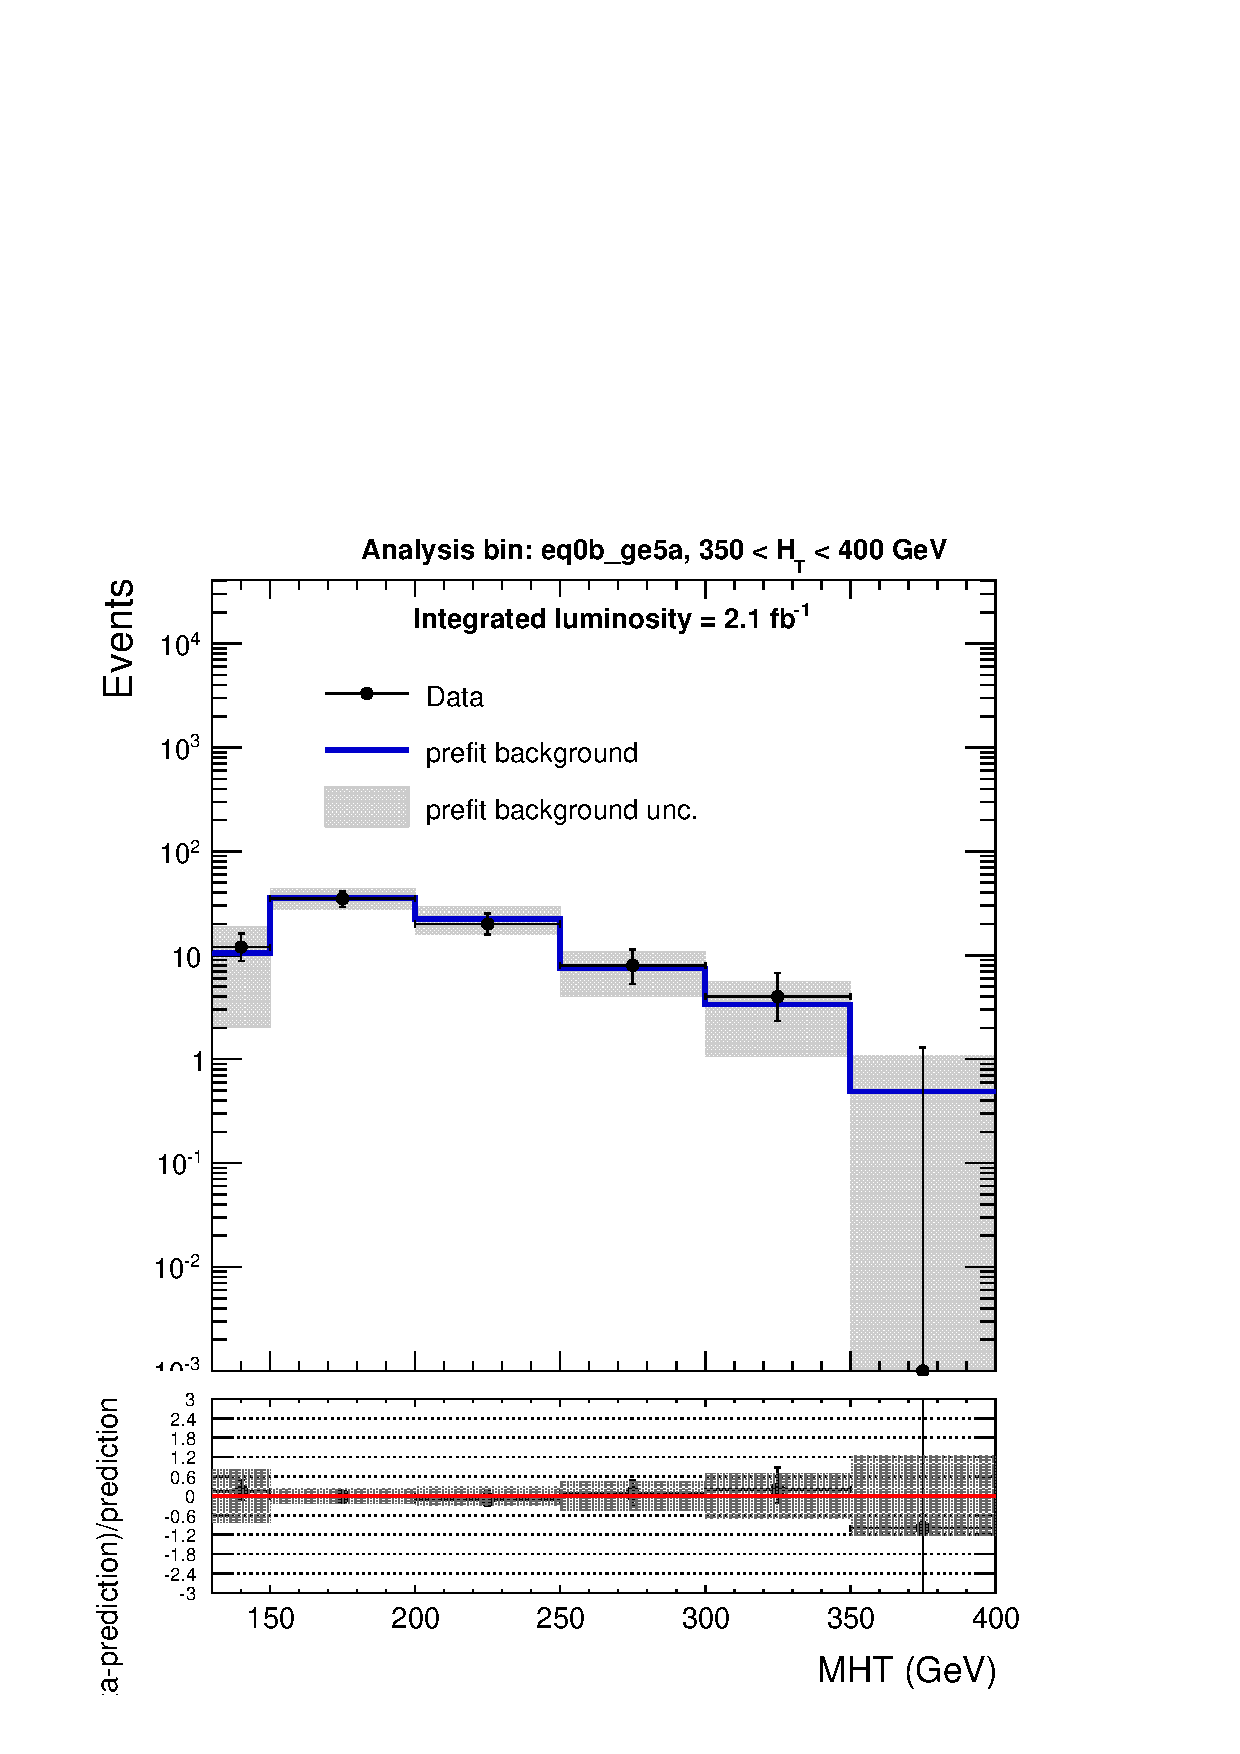
\includegraphics[width=0.25\textwidth]{figures/postFitResults/postFitShapes/postFitShape_eq0b_ge5a_350_400.pdf} }\hspace{1cm}
    \subfigure[$\nj^{\mathrm{asym}}=5$, $\nb=0$, $400 < \scalht < 500 \; \mathrm{GeV}$]{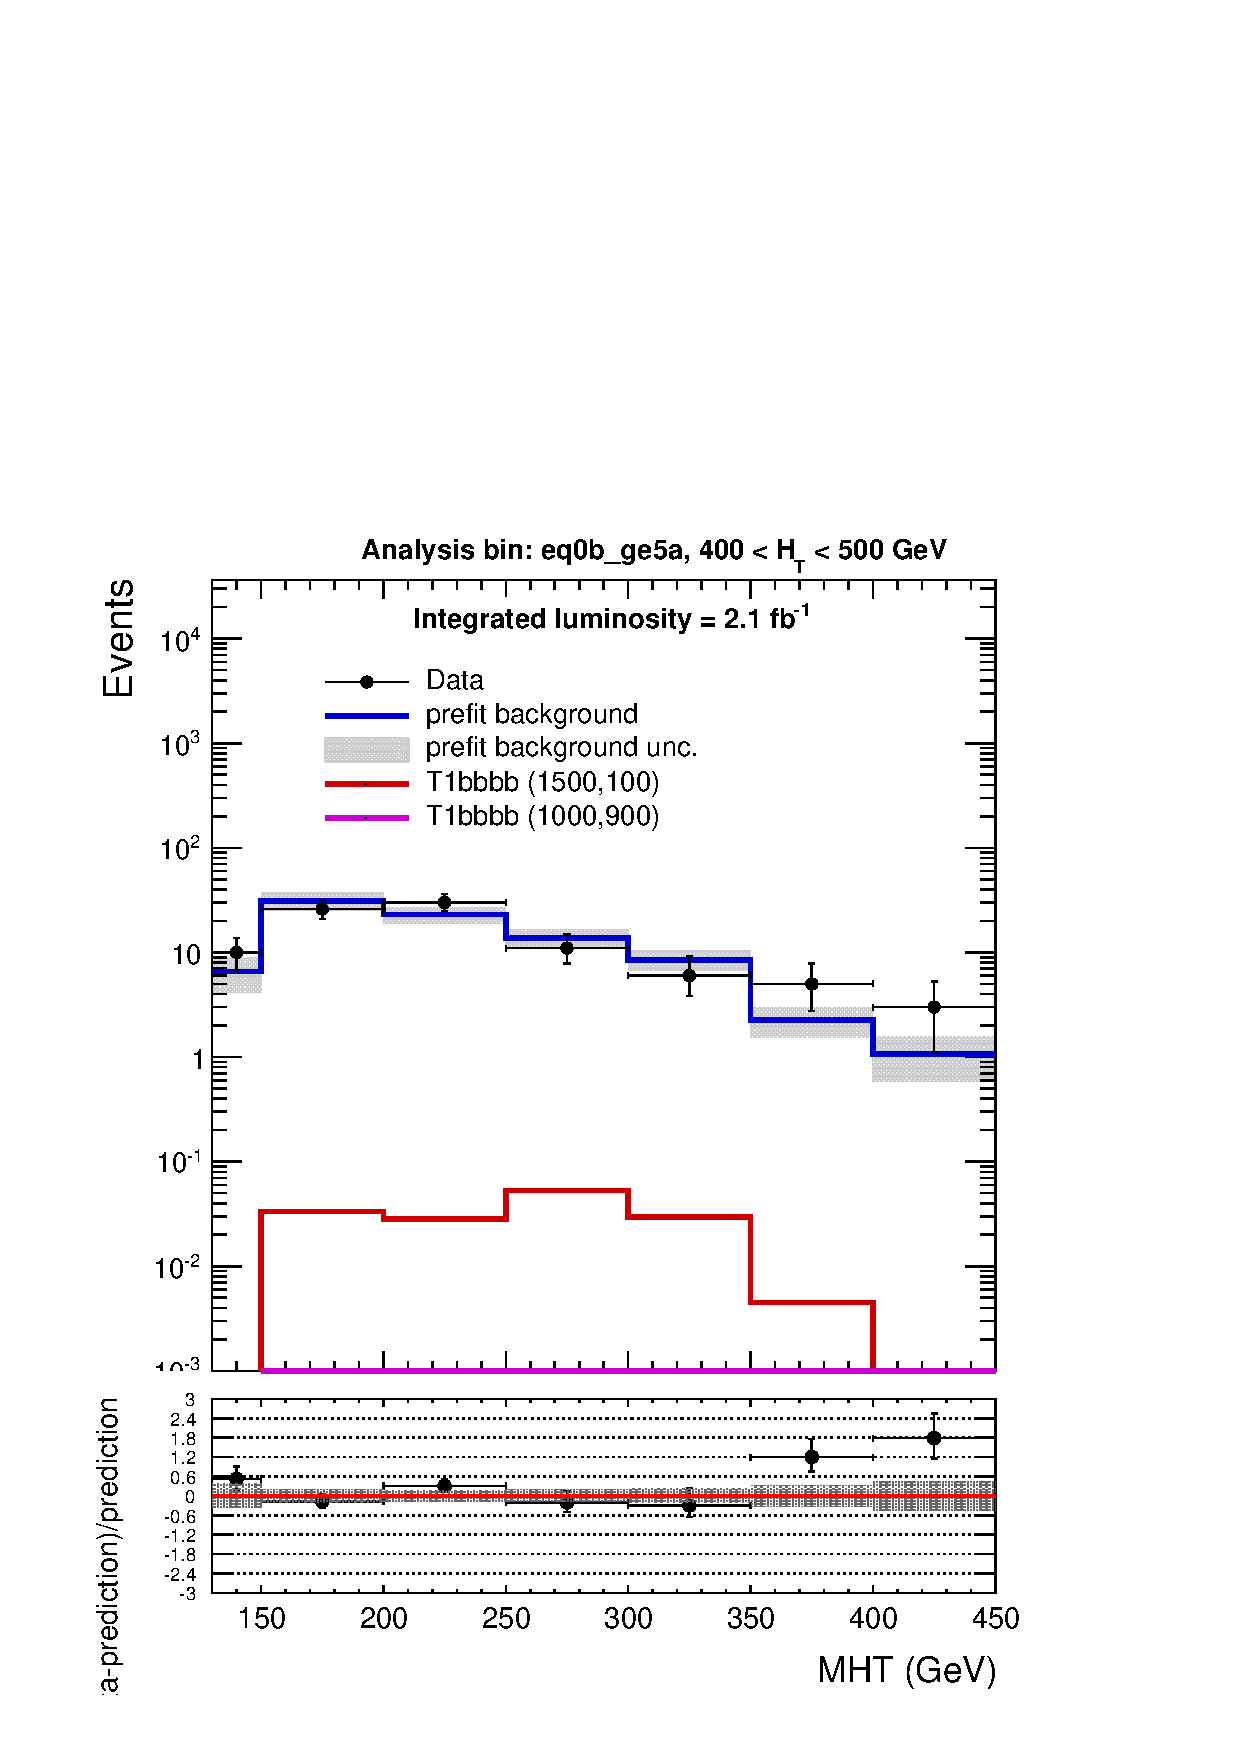
\includegraphics[width=0.25\textwidth]{figures/postFitResults/postFitShapes/postFitShape_eq0b_ge5a_400_500.pdf} }\\
    \subfigure[$\nj^{\mathrm{asym}}=5$, $\nb=0$, $500 < \scalht < 600 \; \mathrm{GeV}$]{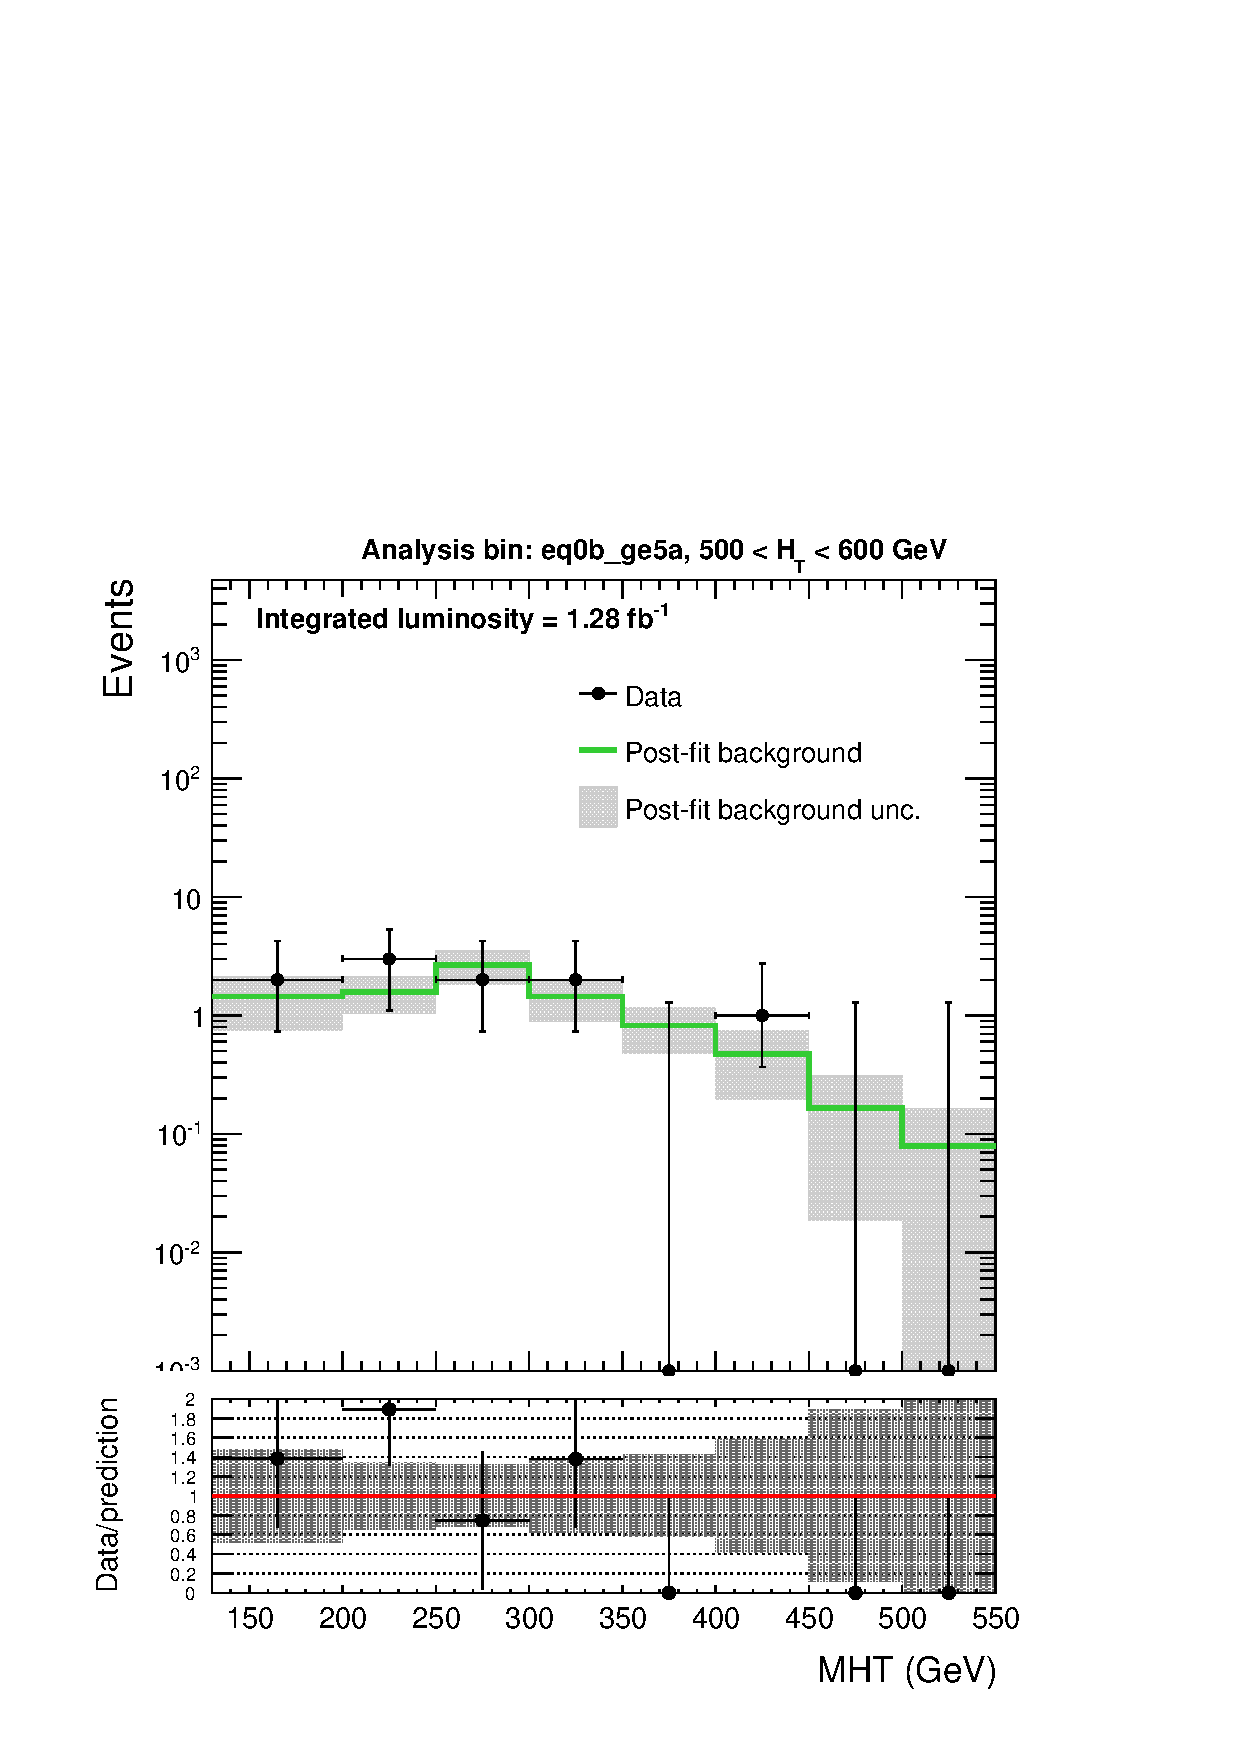
\includegraphics[width=0.25\textwidth]{figures/postFitResults/postFitShapes/postFitShape_eq0b_ge5a_500_600.pdf} }\hspace{1cm}
  \end{center}
\end{figure}



\newpage
\begin{figure}[h!]
\caption{Post-fit \MHT templates for the bin $\nj^{\mathrm{sym}}=5$, $\nb=0$ \label{fig:postFitShapes_eq0b_ge5j}}.
\begin{center}

    \subfigure[$\nj^{\mathrm{sym}}=5$, $\nb=0$, $350 < \scalht < 400 \; \mathrm{GeV}$]{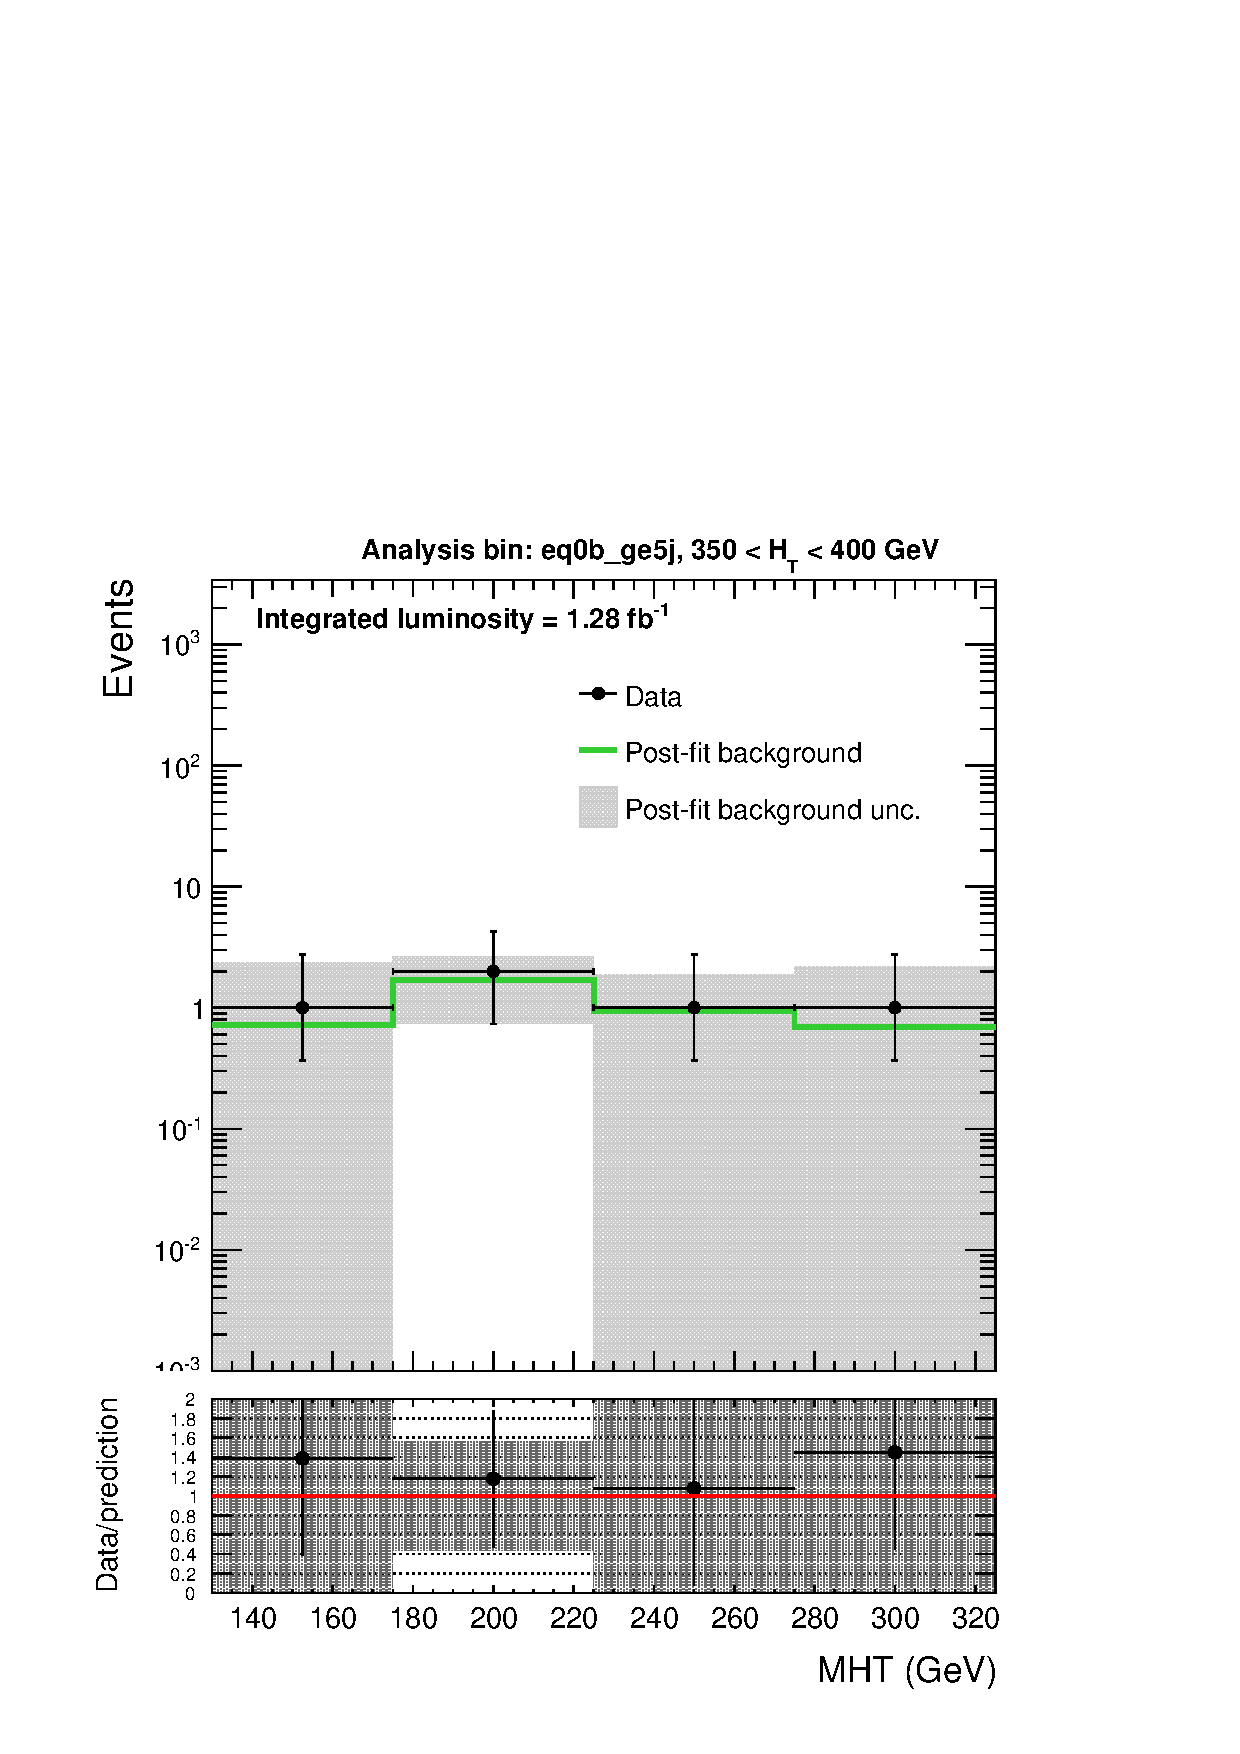
\includegraphics[width=0.25\textwidth]{figures/postFitResults/postFitShapes/postFitShape_eq0b_ge5j_350_400.pdf} }\hspace{1cm}
    \subfigure[$\nj^{\mathrm{sym}}=5$, $\nb=0$, $400 < \scalht < 500 \; \mathrm{GeV}$]{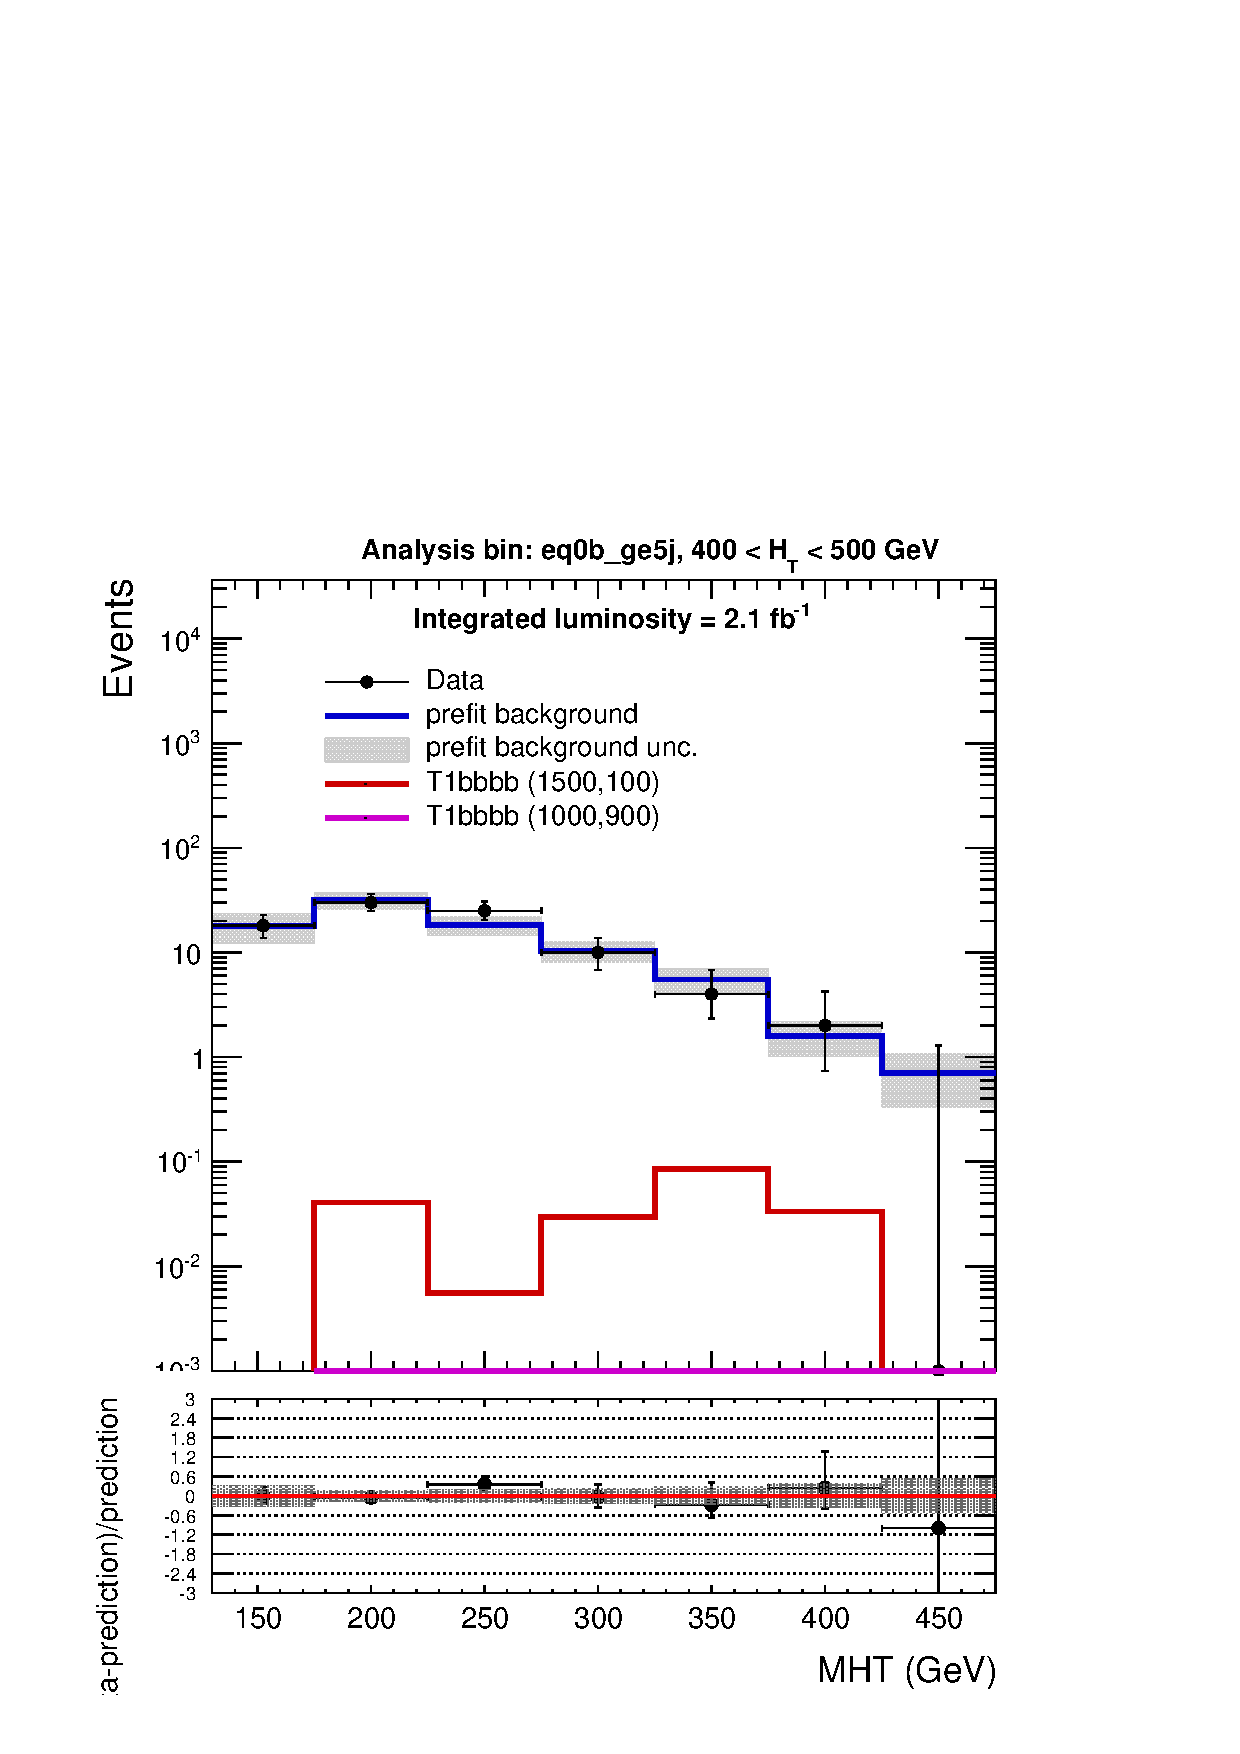
\includegraphics[width=0.25\textwidth]{figures/postFitResults/postFitShapes/postFitShape_eq0b_ge5j_400_500.pdf} }\hspace{1cm}
    \subfigure[$\nj^{\mathrm{sym}}=5$, $\nb=0$, $500 < \scalht < 600 \; \mathrm{GeV}$]{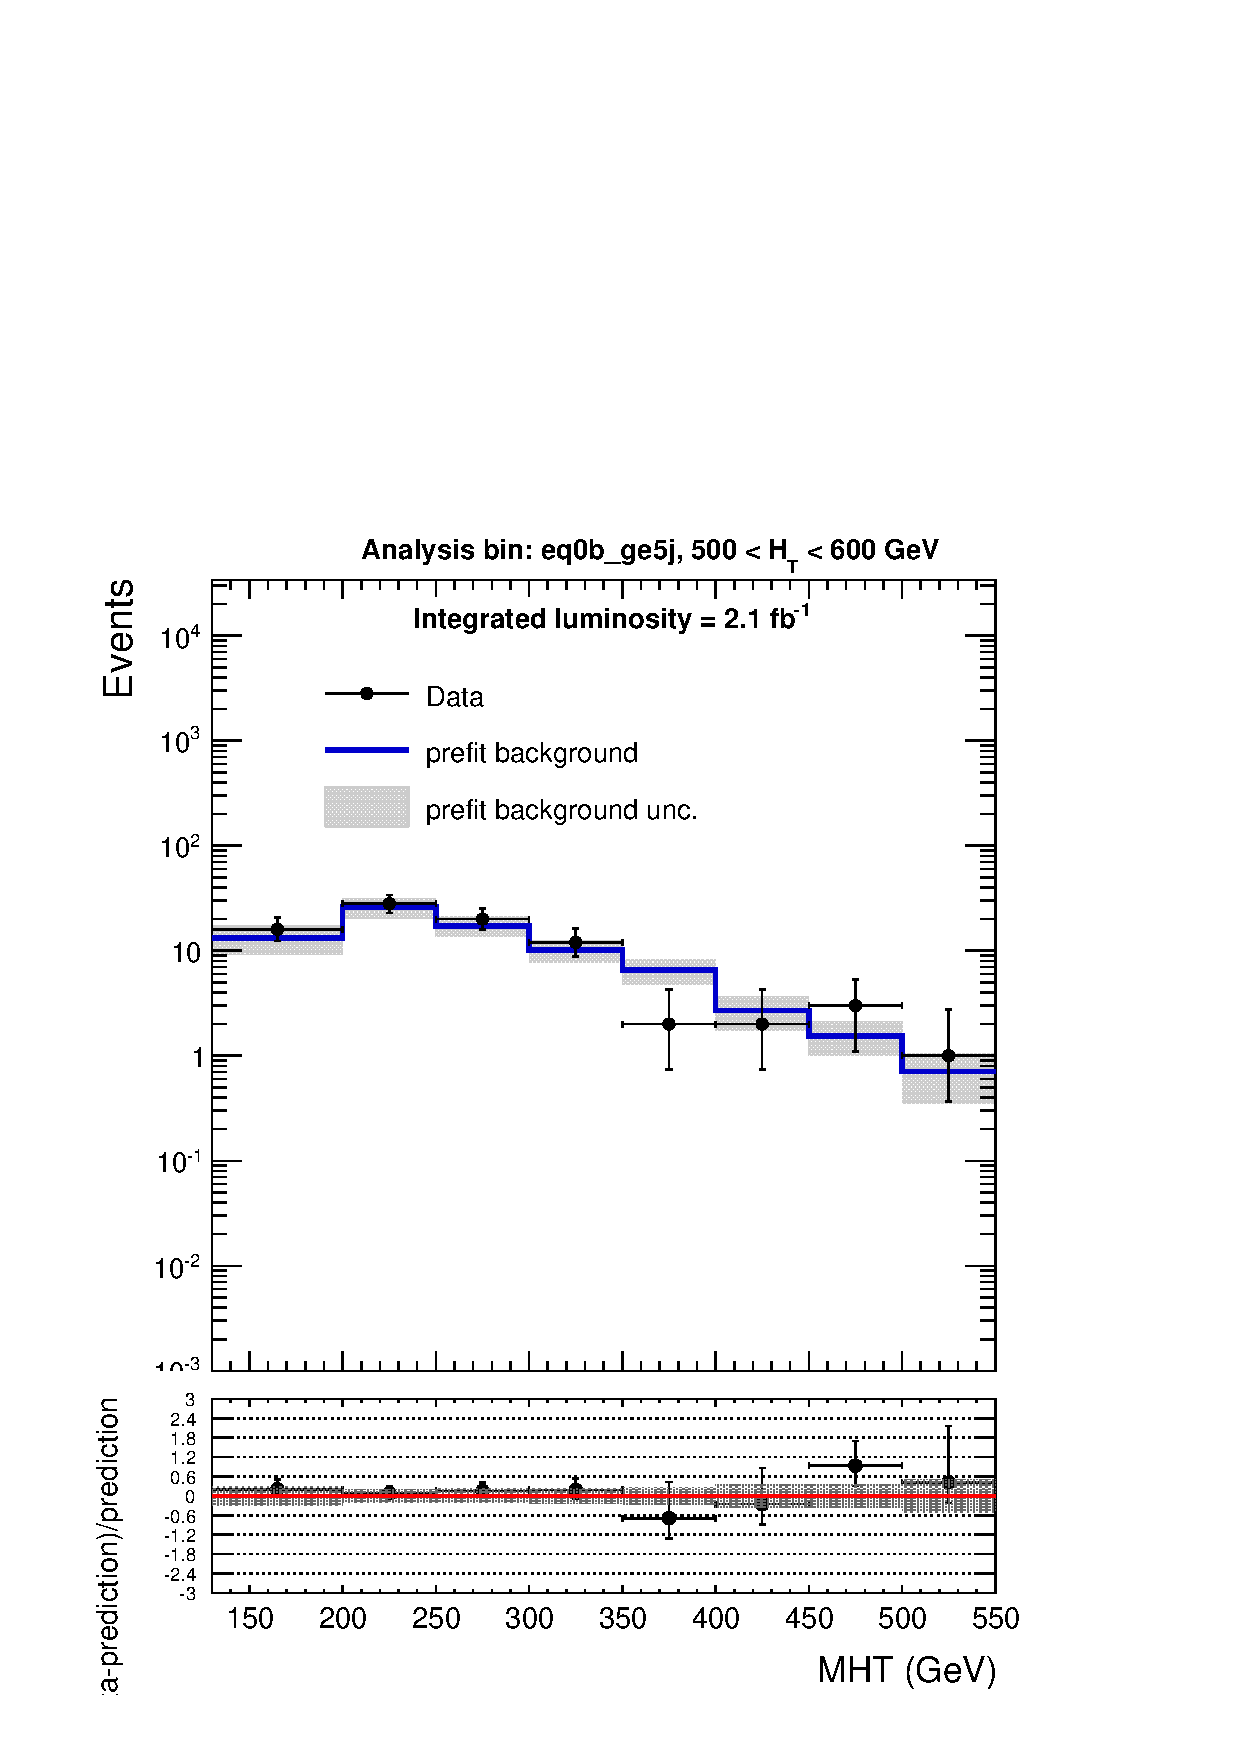
\includegraphics[width=0.25\textwidth]{figures/postFitResults/postFitShapes/postFitShape_eq0b_ge5j_500_600.pdf} }\\
    \subfigure[$\nj^{\mathrm{sym}}=5$, $\nb=0$, $600 < \scalht < 800 \; \mathrm{GeV}$]{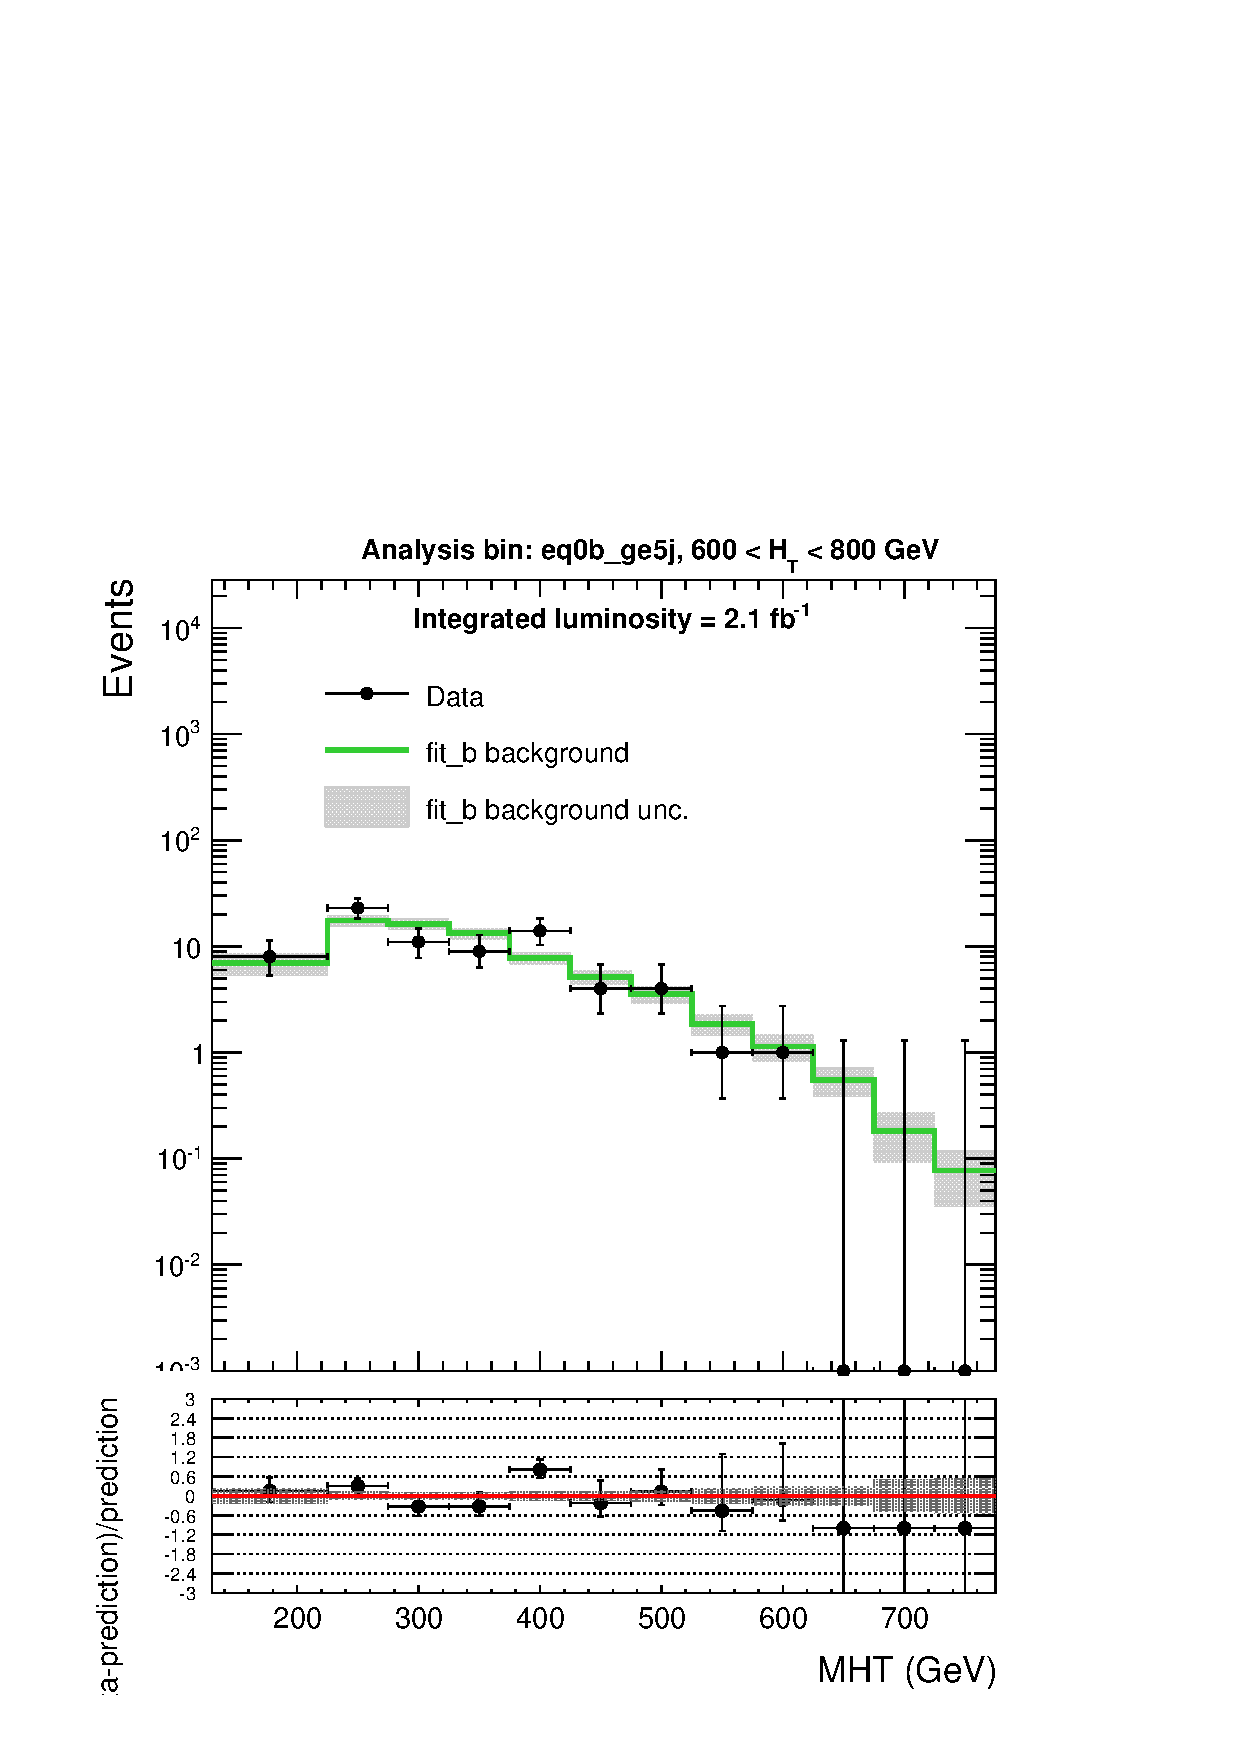
\includegraphics[width=0.25\textwidth]{figures/postFitResults/postFitShapes/postFitShape_eq0b_ge5j_600_800.pdf} }\hspace{1cm}
    \subfigure[$\nj^{\mathrm{sym}}=5$, $\nb=0$, $\scalht > 800 \; \mathrm{GeV}$]{\includegraphics[width=0.25\textwidth]{figures/postFitResults/postFitShapes/postFitShape_eq0b_ge5j_800_Inf.pdf} }\hspace{1cm}
  \end{center}
\end{figure}



\newpage
\begin{figure}[h!]
\caption{Post-fit \MHT templates for the bin $\nj^{\mathrm{asym}}=2$, $\nb=1$ \label{fig:postFitShapes_eq1b_eq2a}}.
\begin{center}

    \subfigure[$\nj^{\mathrm{asym}}=2$, $\nb=1$, $200 < \scalht < 250 \; \mathrm{GeV}$]{\includegraphics[width=0.25\textwidth]{figures/postFitResults/postFitShapes/postFitShape_eq1b_eq2a_200_250.pdf} }\hspace{1cm}
    \subfigure[$\nj^{\mathrm{asym}}=2$, $\nb=1$, $250 < \scalht < 300 \; \mathrm{GeV}$]{\includegraphics[width=0.25\textwidth]{figures/postFitResults/postFitShapes/postFitShape_eq1b_eq2a_250_300.pdf} }\hspace{1cm}
    \subfigure[$\nj^{\mathrm{asym}}=2$, $\nb=1$, $300 < \scalht < 350 \; \mathrm{GeV}$]{\includegraphics[width=0.25\textwidth]{figures/postFitResults/postFitShapes/postFitShape_eq1b_eq2a_300_350.pdf} }\\
    \subfigure[$\nj^{\mathrm{asym}}=2$, $\nb=1$, $350 < \scalht < 400 \; \mathrm{GeV}$]{\includegraphics[width=0.25\textwidth]{figures/postFitResults/postFitShapes/postFitShape_eq1b_eq2a_350_400.pdf} }\hspace{1cm}
    \subfigure[$\nj^{\mathrm{asym}}=2$, $\nb=1$, $400 < \scalht < 500 \; \mathrm{GeV}$]{\includegraphics[width=0.25\textwidth]{figures/postFitResults/postFitShapes/postFitShape_eq1b_eq2a_400_500.pdf} }\hspace{1cm}
    \subfigure[$\nj^{\mathrm{asym}}=2$, $\nb=1$, $500 < \scalht < 600 \; \mathrm{GeV}$]{\includegraphics[width=0.25\textwidth]{figures/postFitResults/postFitShapes/postFitShape_eq1b_eq2a_500_Inf.pdf} }\\
  \end{center}
\end{figure}



\newpage
\begin{figure}[h!]
\caption{Post-fit \MHT templates for the bin $\nj^{\mathrm{sym}}=2$, $\nb=1$ \label{fig:postFitShapes_eq1b_eq2j}}.
\begin{center}

    \subfigure[$\nj^{\mathrm{sym}}=2$, $\nb=1$, $200 < \scalht < 250 \; \mathrm{GeV}$]{\includegraphics[width=0.25\textwidth]{figures/postFitResults/postFitShapes/postFitShape_eq1b_eq2j_200_250.pdf} }\hspace{1cm}
    \subfigure[$\nj^{\mathrm{sym}}=2$, $\nb=1$, $250 < \scalht < 300 \; \mathrm{GeV}$]{\includegraphics[width=0.25\textwidth]{figures/postFitResults/postFitShapes/postFitShape_eq1b_eq2j_250_300.pdf} }\hspace{1cm}
    \subfigure[$\nj^{\mathrm{sym}}=2$, $\nb=1$, $300 < \scalht < 350 \; \mathrm{GeV}$]{\includegraphics[width=0.25\textwidth]{figures/postFitResults/postFitShapes/postFitShape_eq1b_eq2j_300_350.pdf} }\\
    \subfigure[$\nj^{\mathrm{sym}}=2$, $\nb=1$, $350 < \scalht < 400 \; \mathrm{GeV}$]{\includegraphics[width=0.25\textwidth]{figures/postFitResults/postFitShapes/postFitShape_eq1b_eq2j_350_400.pdf} }\hspace{1cm}
    \subfigure[$\nj^{\mathrm{sym}}=2$, $\nb=1$, $400 < \scalht < 500 \; \mathrm{GeV}$]{\includegraphics[width=0.25\textwidth]{figures/postFitResults/postFitShapes/postFitShape_eq1b_eq2j_400_500.pdf} }\hspace{1cm}
    \subfigure[$\nj^{\mathrm{sym}}=2$, $\nb=1$, $500 < \scalht < 600 \; \mathrm{GeV}$]{\includegraphics[width=0.25\textwidth]{figures/postFitResults/postFitShapes/postFitShape_eq1b_eq2j_500_600.pdf} }\\
    \subfigure[$\nj^{\mathrm{sym}}=2$, $\nb=1$, $600 < \scalht < 800 \; \mathrm{GeV}$]{\includegraphics[width=0.25\textwidth]{figures/postFitResults/postFitShapes/postFitShape_eq1b_eq2j_600_800.pdf} }\hspace{1cm}
    \subfigure[$\nj^{\mathrm{sym}}=2$, $\nb=1$, $\scalht > 800 \; \mathrm{GeV}$]{\includegraphics[width=0.25\textwidth]{figures/postFitResults/postFitShapes/postFitShape_eq1b_eq2j_800_Inf.pdf} }\hspace{1cm}
  \end{center}
\end{figure}



\newpage
\begin{figure}[h!]
\caption{Post-fit \MHT templates for the bin $\nj^{\mathrm{asym}}=3$, $\nb=1$ \label{fig:postFitShapes_eq1b_eq3a}}.
\begin{center}

    \subfigure[$\nj^{\mathrm{asym}}=3$, $\nb=1$, $200 < \scalht < 250 \; \mathrm{GeV}$]{\includegraphics[width=0.25\textwidth]{figures/postFitResults/postFitShapes/postFitShape_eq1b_eq3a_200_250.pdf} }\hspace{1cm}
    \subfigure[$\nj^{\mathrm{asym}}=3$, $\nb=1$, $250 < \scalht < 300 \; \mathrm{GeV}$]{\includegraphics[width=0.25\textwidth]{figures/postFitResults/postFitShapes/postFitShape_eq1b_eq3a_250_300.pdf} }\hspace{1cm}
    \subfigure[$\nj^{\mathrm{asym}}=3$, $\nb=1$, $300 < \scalht < 350 \; \mathrm{GeV}$]{\includegraphics[width=0.25\textwidth]{figures/postFitResults/postFitShapes/postFitShape_eq1b_eq3a_300_350.pdf} }\\
    \subfigure[$\nj^{\mathrm{asym}}=3$, $\nb=1$, $350 < \scalht < 400 \; \mathrm{GeV}$]{\includegraphics[width=0.25\textwidth]{figures/postFitResults/postFitShapes/postFitShape_eq1b_eq3a_350_400.pdf} }\hspace{1cm}
    \subfigure[$\nj^{\mathrm{asym}}=3$, $\nb=1$, $400 < \scalht < 500 \; \mathrm{GeV}$]{\includegraphics[width=0.25\textwidth]{figures/postFitResults/postFitShapes/postFitShape_eq1b_eq3a_400_500.pdf} }\hspace{1cm}
    \subfigure[$\nj^{\mathrm{asym}}=3$, $\nb=1$, $500 < \scalht < 600 \; \mathrm{GeV}$]{\includegraphics[width=0.25\textwidth]{figures/postFitResults/postFitShapes/postFitShape_eq1b_eq3a_500_600.pdf} }\\
    \subfigure[$\nj^{\mathrm{asym}}=3$, $\nb=1$, $\scalht > 600 \; \mathrm{GeV}$]{\includegraphics[width=0.25\textwidth]{figures/postFitResults/postFitShapes/postFitShape_eq1b_eq3a_600_Inf.pdf} }\hspace{1cm}
  \end{center}
\end{figure}



\newpage
\begin{figure}[h!]
\caption{Post-fit \MHT templates for the bin $\nj^{\mathrm{sym}}=3$, $\nb=1$ \label{fig:postFitShapes_eq1b_eq3j}}.
\begin{center}

    \subfigure[$\nj^{\mathrm{sym}}=3$, $\nb=1$, $250 < \scalht < 300 \; \mathrm{GeV}$]{\includegraphics[width=0.25\textwidth]{figures/postFitResults/postFitShapes/postFitShape_eq1b_eq3j_250_300.pdf} }\hspace{1cm}
    \subfigure[$\nj^{\mathrm{sym}}=3$, $\nb=1$, $300 < \scalht < 350 \; \mathrm{GeV}$]{\includegraphics[width=0.25\textwidth]{figures/postFitResults/postFitShapes/postFitShape_eq1b_eq3j_300_350.pdf} }\hspace{1cm}
    \subfigure[$\nj^{\mathrm{sym}}=3$, $\nb=1$, $350 < \scalht < 400 \; \mathrm{GeV}$]{\includegraphics[width=0.25\textwidth]{figures/postFitResults/postFitShapes/postFitShape_eq1b_eq3j_350_400.pdf} }\\
    \subfigure[$\nj^{\mathrm{sym}}=3$, $\nb=1$, $400 < \scalht < 500 \; \mathrm{GeV}$]{\includegraphics[width=0.25\textwidth]{figures/postFitResults/postFitShapes/postFitShape_eq1b_eq3j_400_500.pdf} }\hspace{1cm}
    \subfigure[$\nj^{\mathrm{sym}}=3$, $\nb=1$, $500 < \scalht < 600 \; \mathrm{GeV}$]{\includegraphics[width=0.25\textwidth]{figures/postFitResults/postFitShapes/postFitShape_eq1b_eq3j_500_600.pdf} }\hspace{1cm}
    \subfigure[$\nj^{\mathrm{sym}}=3$, $\nb=1$, $600 < \scalht < 800 \; \mathrm{GeV}$]{\includegraphics[width=0.25\textwidth]{figures/postFitResults/postFitShapes/postFitShape_eq1b_eq3j_600_800.pdf} }\\
    \subfigure[$\nj^{\mathrm{sym}}=3$, $\nb=1$, $\scalht > 800 \; \mathrm{GeV}$]{\includegraphics[width=0.25\textwidth]{figures/postFitResults/postFitShapes/postFitShape_eq1b_eq3j_800_Inf.pdf} }\hspace{1cm}
  \end{center}
\end{figure}



\newpage
\begin{figure}[h!]
\caption{Post-fit \MHT templates for the bin $\nj^{\mathrm{asym}}=4$, $\nb=1$ \label{fig:postFitShapes_eq1b_eq4a}}.
\begin{center}

    \subfigure[$\nj^{\mathrm{asym}}=4$, $\nb=1$, $250 < \scalht < 300 \; \mathrm{GeV}$]{\includegraphics[width=0.25\textwidth]{figures/postFitResults/postFitShapes/postFitShape_eq1b_eq4a_250_300.pdf} }\hspace{1cm}
    \subfigure[$\nj^{\mathrm{asym}}=4$, $\nb=1$, $300 < \scalht < 350 \; \mathrm{GeV}$]{\includegraphics[width=0.25\textwidth]{figures/postFitResults/postFitShapes/postFitShape_eq1b_eq4a_300_350.pdf} }\hspace{1cm}
    \subfigure[$\nj^{\mathrm{asym}}=4$, $\nb=1$, $350 < \scalht < 400 \; \mathrm{GeV}$]{\includegraphics[width=0.25\textwidth]{figures/postFitResults/postFitShapes/postFitShape_eq1b_eq4a_350_400.pdf} }\\
    \subfigure[$\nj^{\mathrm{asym}}=4$, $\nb=1$, $400 < \scalht < 500 \; \mathrm{GeV}$]{\includegraphics[width=0.25\textwidth]{figures/postFitResults/postFitShapes/postFitShape_eq1b_eq4a_400_500.pdf} }\hspace{1cm}
    \subfigure[$\nj^{\mathrm{asym}}=4$, $\nb=1$, $500 < \scalht < 600 \; \mathrm{GeV}$]{\includegraphics[width=0.25\textwidth]{figures/postFitResults/postFitShapes/postFitShape_eq1b_eq4a_500_600.pdf} }\hspace{1cm}
    \subfigure[$\nj^{\mathrm{asym}}=4$, $\nb=1$, $\scalht > 600 \; \mathrm{GeV}$]{\includegraphics[width=0.25\textwidth]{figures/postFitResults/postFitShapes/postFitShape_eq1b_eq4a_600_Inf.pdf} }\\
  \end{center}
\end{figure}



\newpage
\begin{figure}[h!]
\caption{Post-fit \MHT templates for the bin $\nj^{\mathrm{sym}}=4$, $\nb=1$ \label{fig:postFitShapes_eq1b_eq4j}}.
\begin{center}

    \subfigure[$\nj^{\mathrm{sym}}=4$, $\nb=1$, $300 < \scalht < 350 \; \mathrm{GeV}$]{\includegraphics[width=0.25\textwidth]{figures/postFitResults/postFitShapes/postFitShape_eq1b_eq4j_300_350.pdf} }\hspace{1cm}
    \subfigure[$\nj^{\mathrm{sym}}=4$, $\nb=1$, $350 < \scalht < 400 \; \mathrm{GeV}$]{\includegraphics[width=0.25\textwidth]{figures/postFitResults/postFitShapes/postFitShape_eq1b_eq4j_350_400.pdf} }\hspace{1cm}
    \subfigure[$\nj^{\mathrm{sym}}=4$, $\nb=1$, $400 < \scalht < 500 \; \mathrm{GeV}$]{\includegraphics[width=0.25\textwidth]{figures/postFitResults/postFitShapes/postFitShape_eq1b_eq4j_400_500.pdf} }\\
    \subfigure[$\nj^{\mathrm{sym}}=4$, $\nb=1$, $500 < \scalht < 600 \; \mathrm{GeV}$]{\includegraphics[width=0.25\textwidth]{figures/postFitResults/postFitShapes/postFitShape_eq1b_eq4j_500_600.pdf} }\hspace{1cm}
    \subfigure[$\nj^{\mathrm{sym}}=4$, $\nb=1$, $600 < \scalht < 800 \; \mathrm{GeV}$]{\includegraphics[width=0.25\textwidth]{figures/postFitResults/postFitShapes/postFitShape_eq1b_eq4j_600_800.pdf} }\hspace{1cm}
    \subfigure[$\nj^{\mathrm{sym}}=4$, $\nb=1$, $\scalht > 800 \; \mathrm{GeV}$]{\includegraphics[width=0.25\textwidth]{figures/postFitResults/postFitShapes/postFitShape_eq1b_eq4j_800_Inf.pdf} }\\
  \end{center}
\end{figure}



\newpage
\begin{figure}[h!]
\caption{Post-fit \MHT templates for the bin $\nj^{\mathrm{asym}}=5$, $\nb=1$ \label{fig:postFitShapes_eq1b_ge5a}}.
\begin{center}

    \subfigure[$\nj^{\mathrm{asym}}=5$, $\nb=1$, $300 < \scalht < 350 \; \mathrm{GeV}$]{\includegraphics[width=0.25\textwidth]{figures/postFitResults/postFitShapes/postFitShape_eq1b_ge5a_300_350.pdf} }\hspace{1cm}
    \subfigure[$\nj^{\mathrm{asym}}=5$, $\nb=1$, $350 < \scalht < 400 \; \mathrm{GeV}$]{\includegraphics[width=0.25\textwidth]{figures/postFitResults/postFitShapes/postFitShape_eq1b_ge5a_350_400.pdf} }\hspace{1cm}
    \subfigure[$\nj^{\mathrm{asym}}=5$, $\nb=1$, $400 < \scalht < 500 \; \mathrm{GeV}$]{\includegraphics[width=0.25\textwidth]{figures/postFitResults/postFitShapes/postFitShape_eq1b_ge5a_400_500.pdf} }\\
    \subfigure[$\nj^{\mathrm{asym}}=5$, $\nb=1$, $500 < \scalht < 600 \; \mathrm{GeV}$]{\includegraphics[width=0.25\textwidth]{figures/postFitResults/postFitShapes/postFitShape_eq1b_ge5a_500_600.pdf} }\hspace{1cm}
    \subfigure[$\nj^{\mathrm{asym}}=5$, $\nb=1$, $\scalht > 600 \; \mathrm{GeV}$]{\includegraphics[width=0.25\textwidth]{figures/postFitResults/postFitShapes/postFitShape_eq1b_ge5a_600_Inf.pdf} }\hspace{1cm}
  \end{center}
\end{figure}



\newpage
\begin{figure}[h!]
\caption{Post-fit \MHT templates for the bin $\nj^{\mathrm{sym}}=5$, $\nb=1$ \label{fig:postFitShapes_eq1b_ge5j}}.
\begin{center}

    \subfigure[$\nj^{\mathrm{sym}}=5$, $\nb=1$, $400 < \scalht < 500 \; \mathrm{GeV}$]{\includegraphics[width=0.25\textwidth]{figures/postFitResults/postFitShapes/postFitShape_eq1b_ge5j_400_500.pdf} }\hspace{1cm}
    \subfigure[$\nj^{\mathrm{sym}}=5$, $\nb=1$, $500 < \scalht < 600 \; \mathrm{GeV}$]{\includegraphics[width=0.25\textwidth]{figures/postFitResults/postFitShapes/postFitShape_eq1b_ge5j_500_600.pdf} }\hspace{1cm}
    \subfigure[$\nj^{\mathrm{sym}}=5$, $\nb=1$, $600 < \scalht < 800 \; \mathrm{GeV}$]{\includegraphics[width=0.25\textwidth]{figures/postFitResults/postFitShapes/postFitShape_eq1b_ge5j_600_800.pdf} }\\
    \subfigure[$\nj^{\mathrm{sym}}=5$, $\nb=1$, $\scalht > 800 \; \mathrm{GeV}$]{\includegraphics[width=0.25\textwidth]{figures/postFitResults/postFitShapes/postFitShape_eq1b_ge5j_800_Inf.pdf} }\hspace{1cm}
  \end{center}
\end{figure}



\newpage
\begin{figure}[h!]
\caption{Post-fit \MHT templates for the bin $\nj^{\mathrm{asym}}=2$, $\nb=2$ \label{fig:postFitShapes_eq2b_eq2a}}.
\begin{center}

    \subfigure[$\nj^{\mathrm{asym}}=2$, $\nb=2$, $200 < \scalht < 250 \; \mathrm{GeV}$]{\includegraphics[width=0.25\textwidth]{figures/postFitResults/postFitShapes/postFitShape_eq2b_eq2a_200_250.pdf} }\hspace{1cm}
    \subfigure[$\nj^{\mathrm{asym}}=2$, $\nb=2$, $250 < \scalht < 300 \; \mathrm{GeV}$]{\includegraphics[width=0.25\textwidth]{figures/postFitResults/postFitShapes/postFitShape_eq2b_eq2a_250_300.pdf} }\hspace{1cm}
    \subfigure[$\nj^{\mathrm{asym}}=2$, $\nb=2$, $300 < \scalht < 350 \; \mathrm{GeV}$]{\includegraphics[width=0.25\textwidth]{figures/postFitResults/postFitShapes/postFitShape_eq2b_eq2a_300_350.pdf} }\\
  \end{center}
\end{figure}



\newpage
\begin{figure}[h!]
\caption{Post-fit \MHT templates for the bin $\nj^{\mathrm{asym}}=3$, $\nb=2$ \label{fig:postFitShapes_eq2b_eq3a}}.
\begin{center}

    \subfigure[$\nj^{\mathrm{asym}}=3$, $\nb=2$, $200 < \scalht < 250 \; \mathrm{GeV}$]{\includegraphics[width=0.25\textwidth]{figures/postFitResults/postFitShapes/postFitShape_eq2b_eq3a_200_250.pdf} }\hspace{1cm}
    \subfigure[$\nj^{\mathrm{asym}}=3$, $\nb=2$, $250 < \scalht < 300 \; \mathrm{GeV}$]{\includegraphics[width=0.25\textwidth]{figures/postFitResults/postFitShapes/postFitShape_eq2b_eq3a_250_300.pdf} }\hspace{1cm}
    \subfigure[$\nj^{\mathrm{asym}}=3$, $\nb=2$, $300 < \scalht < 350 \; \mathrm{GeV}$]{\includegraphics[width=0.25\textwidth]{figures/postFitResults/postFitShapes/postFitShape_eq2b_eq3a_300_350.pdf} }\\
    \subfigure[$\nj^{\mathrm{asym}}=3$, $\nb=2$, $350 < \scalht < 400 \; \mathrm{GeV}$]{\includegraphics[width=0.25\textwidth]{figures/postFitResults/postFitShapes/postFitShape_eq2b_eq3a_350_400.pdf} }\hspace{1cm}
    \subfigure[$\nj^{\mathrm{asym}}=3$, $\nb=2$, $400 < \scalht < 500 \; \mathrm{GeV}$]{\includegraphics[width=0.25\textwidth]{figures/postFitResults/postFitShapes/postFitShape_eq2b_eq3a_400_500.pdf} }\hspace{1cm}
  \end{center}
\end{figure}



\newpage
\begin{figure}[h!]
\caption{Post-fit \MHT templates for the bin $\nj^{\mathrm{sym}}=3$, $\nb=2$ \label{fig:postFitShapes_eq2b_eq3j}}.
\begin{center}

    \subfigure[$\nj^{\mathrm{sym}}=3$, $\nb=2$, $250 < \scalht < 300 \; \mathrm{GeV}$]{\includegraphics[width=0.25\textwidth]{figures/postFitResults/postFitShapes/postFitShape_eq2b_eq3j_250_300.pdf} }\hspace{1cm}
    \subfigure[$\nj^{\mathrm{sym}}=3$, $\nb=2$, $300 < \scalht < 350 \; \mathrm{GeV}$]{\includegraphics[width=0.25\textwidth]{figures/postFitResults/postFitShapes/postFitShape_eq2b_eq3j_300_350.pdf} }\hspace{1cm}
    \subfigure[$\nj^{\mathrm{sym}}=3$, $\nb=2$, $350 < \scalht < 400 \; \mathrm{GeV}$]{\includegraphics[width=0.25\textwidth]{figures/postFitResults/postFitShapes/postFitShape_eq2b_eq3j_350_400.pdf} }\\
    \subfigure[$\nj^{\mathrm{sym}}=3$, $\nb=2$, $400 < \scalht < 500 \; \mathrm{GeV}$]{\includegraphics[width=0.25\textwidth]{figures/postFitResults/postFitShapes/postFitShape_eq2b_eq3j_400_500.pdf} }\hspace{1cm}
    \subfigure[$\nj^{\mathrm{sym}}=3$, $\nb=2$, $500 < \scalht < 600 \; \mathrm{GeV}$]{\includegraphics[width=0.25\textwidth]{figures/postFitResults/postFitShapes/postFitShape_eq2b_eq3j_500_600.pdf} }\hspace{1cm}
    \subfigure[$\nj^{\mathrm{sym}}=3$, $\nb=2$, $600 < \scalht < 800 \; \mathrm{GeV}$]{\includegraphics[width=0.25\textwidth]{figures/postFitResults/postFitShapes/postFitShape_eq2b_eq3j_600_800.pdf} }\\
    \subfigure[$\nj^{\mathrm{sym}}=3$, $\nb=2$, $\scalht > 800 \; \mathrm{GeV}$]{\includegraphics[width=0.25\textwidth]{figures/postFitResults/postFitShapes/postFitShape_eq2b_eq3j_800_Inf.pdf} }\hspace{1cm}
  \end{center}
\end{figure}



\newpage
\begin{figure}[h!]
\caption{Post-fit \MHT templates for the bin $\nj^{\mathrm{asym}}=4$, $\nb=2$ \label{fig:postFitShapes_eq2b_eq4a}}.
\begin{center}

    \subfigure[$\nj^{\mathrm{asym}}=4$, $\nb=2$, $250 < \scalht < 300 \; \mathrm{GeV}$]{\includegraphics[width=0.25\textwidth]{figures/postFitResults/postFitShapes/postFitShape_eq2b_eq4a_250_300.pdf} }\hspace{1cm}
    \subfigure[$\nj^{\mathrm{asym}}=4$, $\nb=2$, $300 < \scalht < 350 \; \mathrm{GeV}$]{\includegraphics[width=0.25\textwidth]{figures/postFitResults/postFitShapes/postFitShape_eq2b_eq4a_300_350.pdf} }\hspace{1cm}
    \subfigure[$\nj^{\mathrm{asym}}=4$, $\nb=2$, $350 < \scalht < 400 \; \mathrm{GeV}$]{\includegraphics[width=0.25\textwidth]{figures/postFitResults/postFitShapes/postFitShape_eq2b_eq4a_350_400.pdf} }\\
    \subfigure[$\nj^{\mathrm{asym}}=4$, $\nb=2$, $400 < \scalht < 500 \; \mathrm{GeV}$]{\includegraphics[width=0.25\textwidth]{figures/postFitResults/postFitShapes/postFitShape_eq2b_eq4a_400_500.pdf} }\hspace{1cm}
  \end{center}
\end{figure}



\newpage
\begin{figure}[h!]
\caption{Post-fit \MHT templates for the bin $\nj^{\mathrm{sym}}=4$, $\nb=2$ \label{fig:postFitShapes_eq2b_eq4j}}.
\begin{center}

    \subfigure[$\nj^{\mathrm{sym}}=4$, $\nb=2$, $350 < \scalht < 400 \; \mathrm{GeV}$]{\includegraphics[width=0.25\textwidth]{figures/postFitResults/postFitShapes/postFitShape_eq2b_eq4j_350_400.pdf} }\hspace{1cm}
    \subfigure[$\nj^{\mathrm{sym}}=4$, $\nb=2$, $400 < \scalht < 500 \; \mathrm{GeV}$]{\includegraphics[width=0.25\textwidth]{figures/postFitResults/postFitShapes/postFitShape_eq2b_eq4j_400_500.pdf} }\hspace{1cm}
    \subfigure[$\nj^{\mathrm{sym}}=4$, $\nb=2$, $500 < \scalht < 600 \; \mathrm{GeV}$]{\includegraphics[width=0.25\textwidth]{figures/postFitResults/postFitShapes/postFitShape_eq2b_eq4j_500_600.pdf} }\\
    \subfigure[$\nj^{\mathrm{sym}}=4$, $\nb=2$, $600 < \scalht < 800 \; \mathrm{GeV}$]{\includegraphics[width=0.25\textwidth]{figures/postFitResults/postFitShapes/postFitShape_eq2b_eq4j_600_800.pdf} }\hspace{1cm}
    \subfigure[$\nj^{\mathrm{sym}}=4$, $\nb=2$, $\scalht > 800 \; \mathrm{GeV}$]{\includegraphics[width=0.25\textwidth]{figures/postFitResults/postFitShapes/postFitShape_eq2b_eq4j_800_Inf.pdf} }\\
  \end{center}
\end{figure}



\newpage
\begin{figure}[h!]
\caption{Post-fit \MHT templates for the bin $\nj^{\mathrm{asym}}=5$, $\nb=2$ \label{fig:postFitShapes_eq2b_ge5a}}.
\begin{center}

    \subfigure[$\nj^{\mathrm{asym}}=5$, $\nb=2$, $350 < \scalht < 400 \; \mathrm{GeV}$]{\includegraphics[width=0.25\textwidth]{figures/postFitResults/postFitShapes/postFitShape_eq2b_ge5a_350_400.pdf} }\hspace{1cm}
    \subfigure[$\nj^{\mathrm{asym}}=5$, $\nb=2$, $400 < \scalht < 500 \; \mathrm{GeV}$]{\includegraphics[width=0.25\textwidth]{figures/postFitResults/postFitShapes/postFitShape_eq2b_ge5a_400_500.pdf} }\hspace{1cm}
    \subfigure[$\nj^{\mathrm{asym}}=5$, $\nb=2$, $500 < \scalht < 600 \; \mathrm{GeV}$]{\includegraphics[width=0.25\textwidth]{figures/postFitResults/postFitShapes/postFitShape_eq2b_ge5a_500_600.pdf} }\\
  \end{center}
\end{figure}



\newpage
\begin{figure}[h!]
\caption{Post-fit \MHT templates for the bin $\nj^{\mathrm{sym}}=5$, $\nb=2$ \label{fig:postFitShapes_eq2b_ge5j}}.
\begin{center}

    \subfigure[$\nj^{\mathrm{sym}}=5$, $\nb=2$, $400 < \scalht < 500 \; \mathrm{GeV}$]{\includegraphics[width=0.25\textwidth]{figures/postFitResults/postFitShapes/postFitShape_eq2b_ge5j_400_500.pdf} }\hspace{1cm}
    \subfigure[$\nj^{\mathrm{sym}}=5$, $\nb=2$, $500 < \scalht < 600 \; \mathrm{GeV}$]{\includegraphics[width=0.25\textwidth]{figures/postFitResults/postFitShapes/postFitShape_eq2b_ge5j_500_600.pdf} }\hspace{1cm}
    \subfigure[$\nj^{\mathrm{sym}}=5$, $\nb=2$, $600 < \scalht < 800 \; \mathrm{GeV}$]{\includegraphics[width=0.25\textwidth]{figures/postFitResults/postFitShapes/postFitShape_eq2b_ge5j_600_800.pdf} }\\
    \subfigure[$\nj^{\mathrm{sym}}=5$, $\nb=2$, $\scalht > 800 \; \mathrm{GeV}$]{\includegraphics[width=0.25\textwidth]{figures/postFitResults/postFitShapes/postFitShape_eq2b_ge5j_800_Inf.pdf} }\hspace{1cm}
  \end{center}
\end{figure}


\newpage
\begin{figure}[h!]
\caption{Post-fit \MHT templates for the bin $\nj^{\mathrm{sym}}=5$, $\nb\ge 3$ \label{fig:postFitShapes_ge3b_ge5j}}.
\begin{center}
    \subfigure[$\nj^{\mathrm{sym}}=5$, $\nb=3$, $\scalht > 800 \; \mathrm{GeV}$]{\includegraphics[width=0.25\textwidth]{figures/postFitResults/postFitShapes/postFitShape_ge3b_ge5j_800_Inf.pdf} }\hspace{1cm}
\end{center}
\end{figure}
